\chapter{Nominal MC Distributions}\label{app:nomMC}

The 2D nominal, uniformly-binned runs 2--9 MC distributions are shown in Figure \ref{fig:2dnomall}. 

\begin{figure}
\centering
\begin{subfigure}{.32\textwidth}
  \centering
  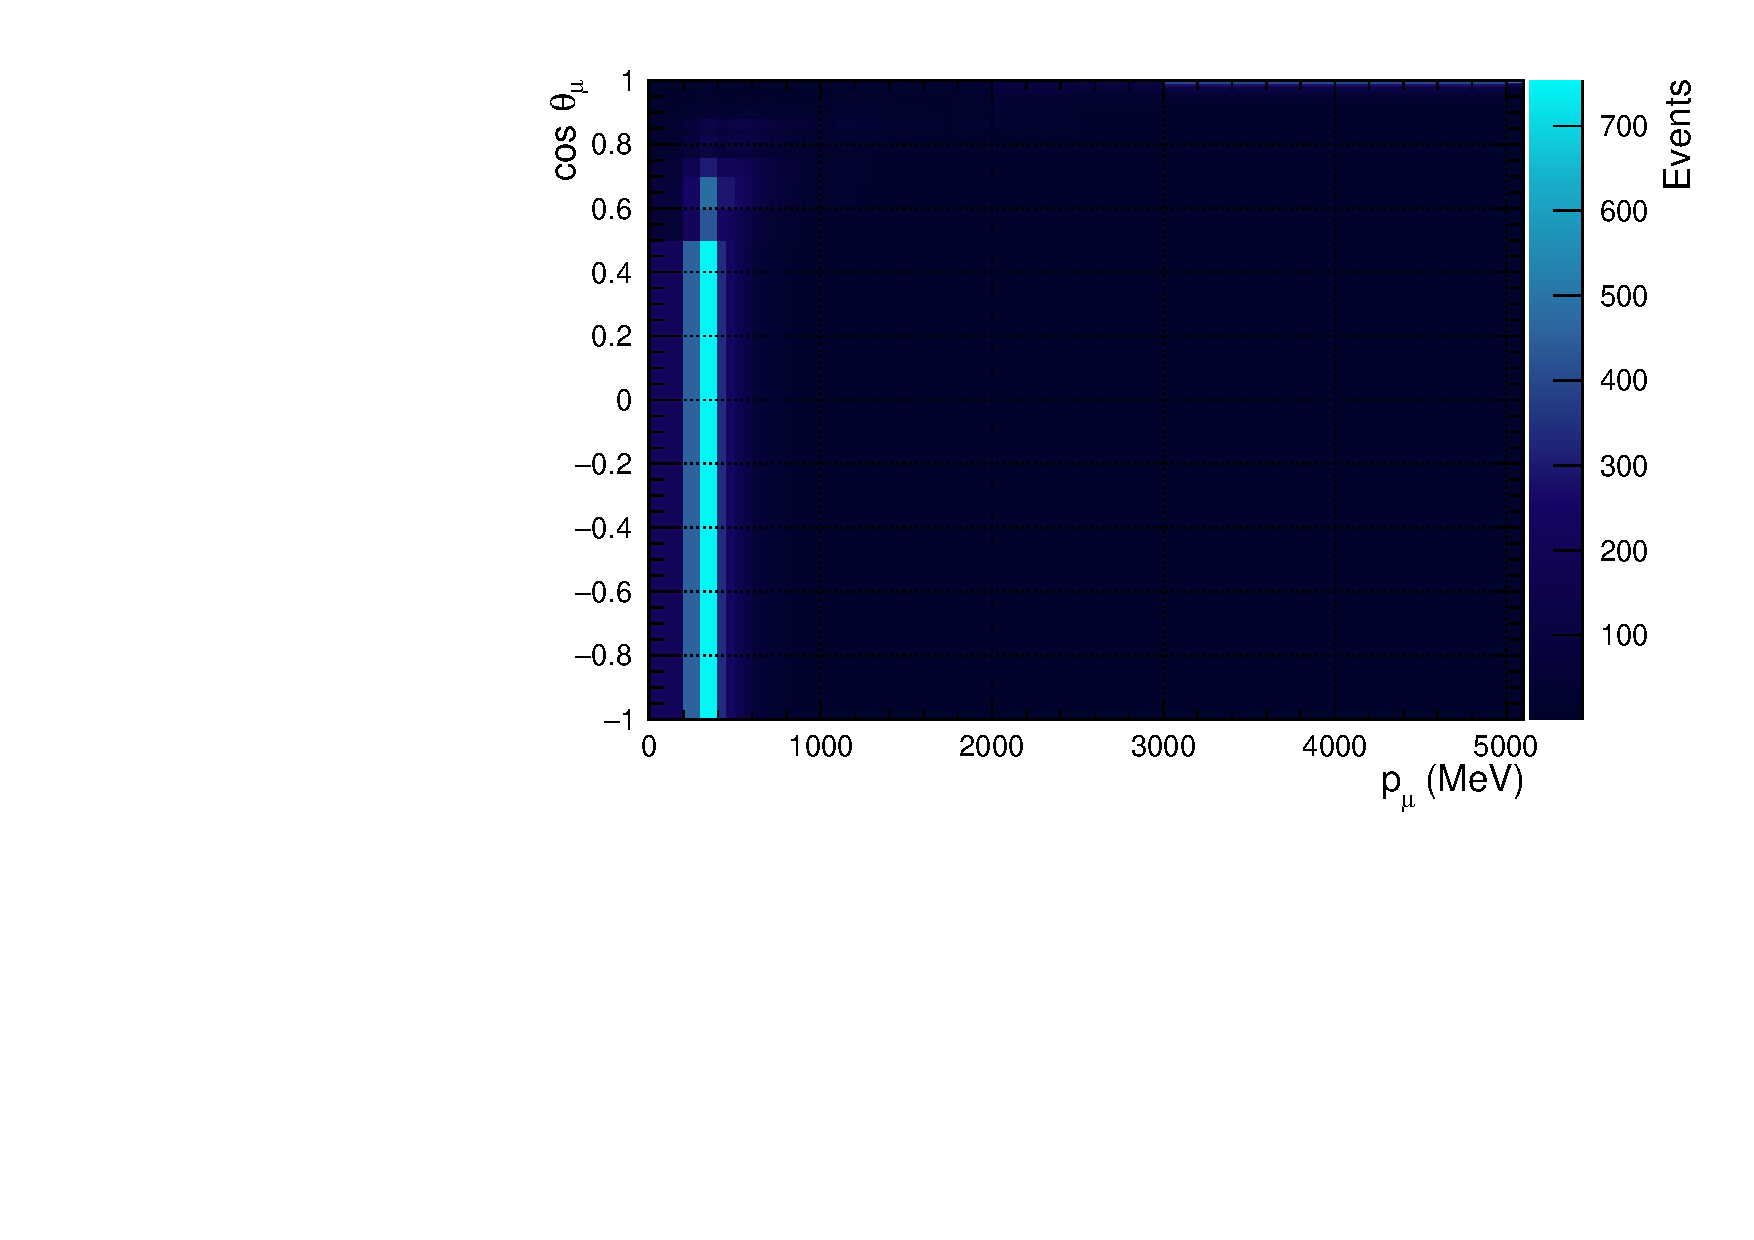
\includegraphics[width=0.95\linewidth]{figs/NomMC_MC_FGD1_numuCC_0pi}
  \caption{FGD1 FHC $\nu_{\mu}$ 0$\pi$}
  \label{fig:2d_FGD1_numuCC_0pi}
\end{subfigure}
\begin{subfigure}{.32\textwidth}
  \centering
  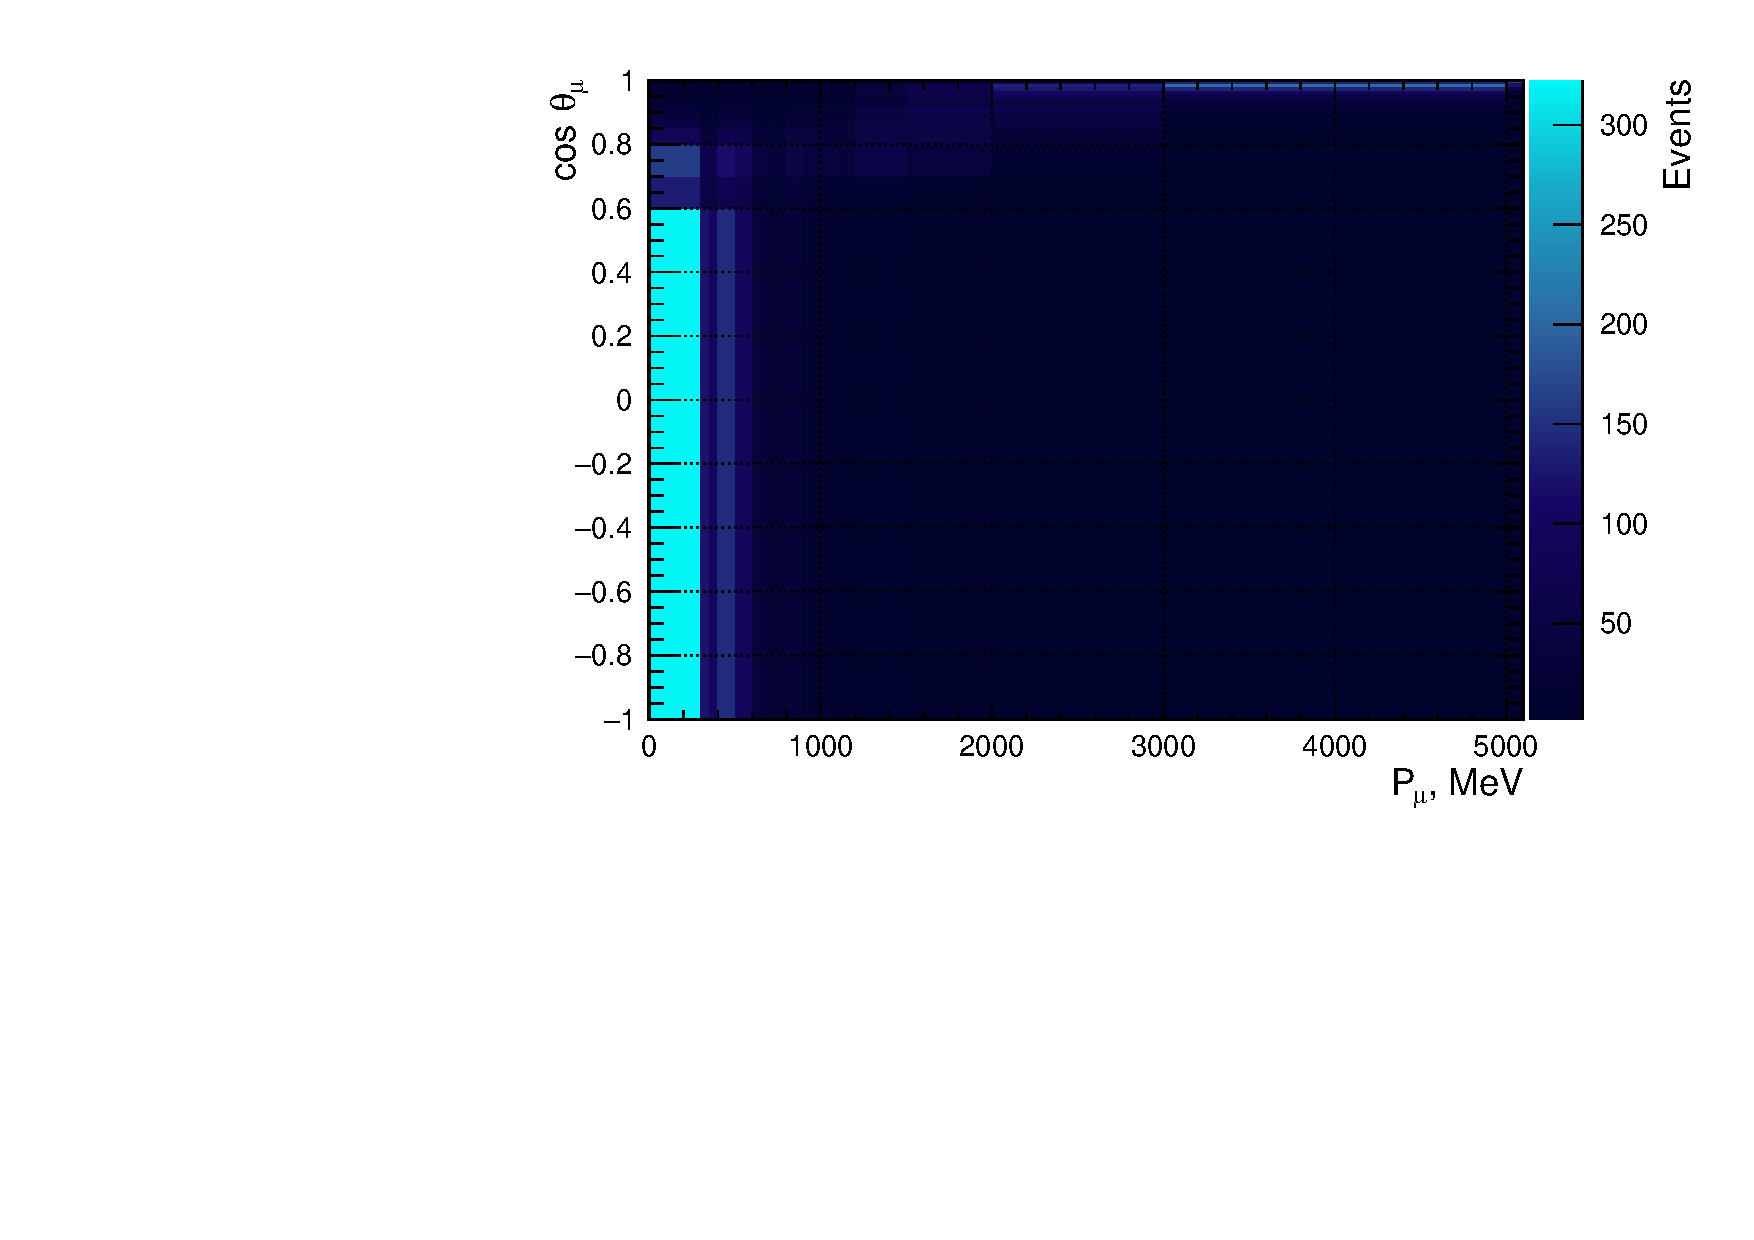
\includegraphics[width=0.95\linewidth]{figs/NomMC_MC_FGD1_numuCC_1pi}
  \caption{FGD1 FHC $\nu_{\mu}$ 1$\pi$}
  \label{fig:2d_FGD1_numuCC_1pi}
\end{subfigure}
\begin{subfigure}{.32\textwidth}
  \centering
  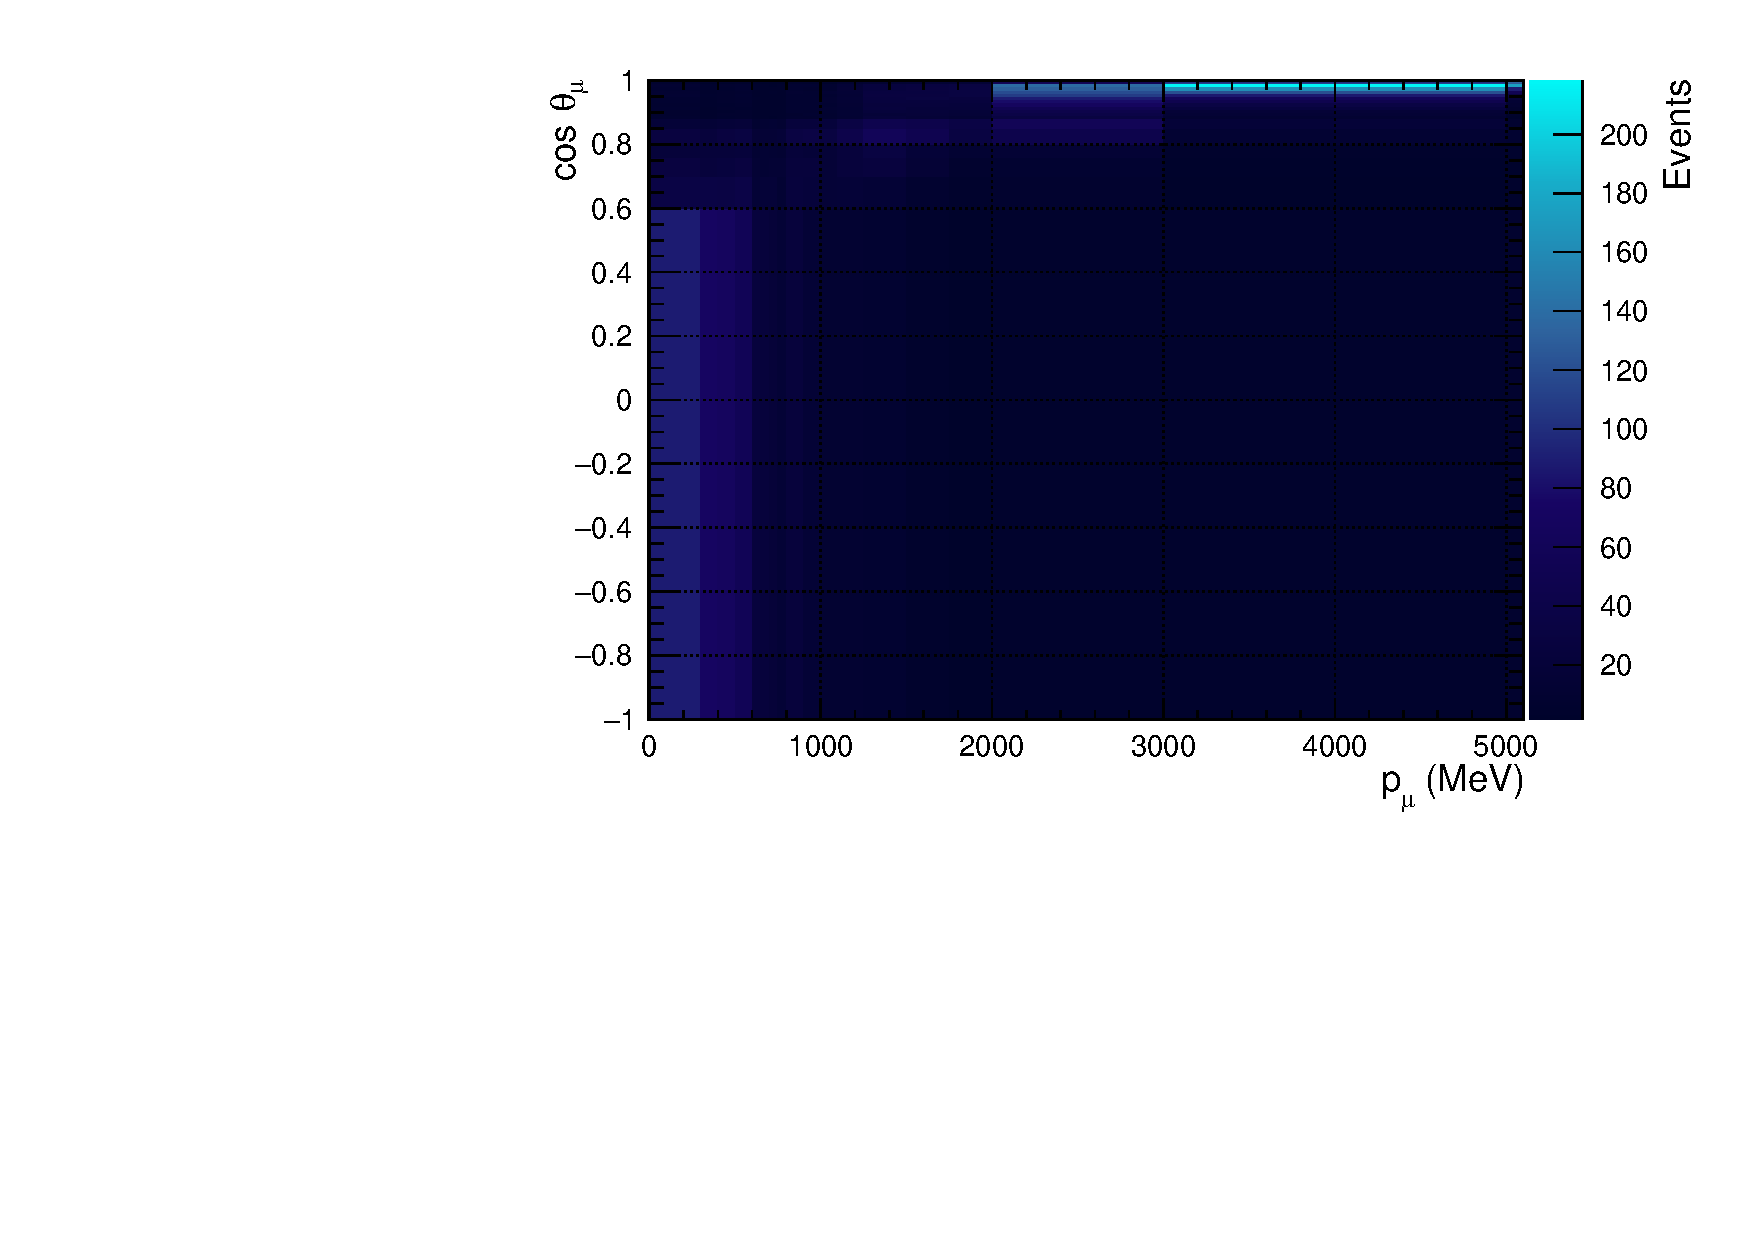
\includegraphics[width=0.95\linewidth]{figs/NomMC_MC_FGD1_numuCC_other}
  \caption{FGD1 FHC $\nu_{\mu}$ Other}
  \label{fig:2d_FGD1_numuCC_other}
\end{subfigure}
\centering
\begin{subfigure}{.32\textwidth}
  \centering
  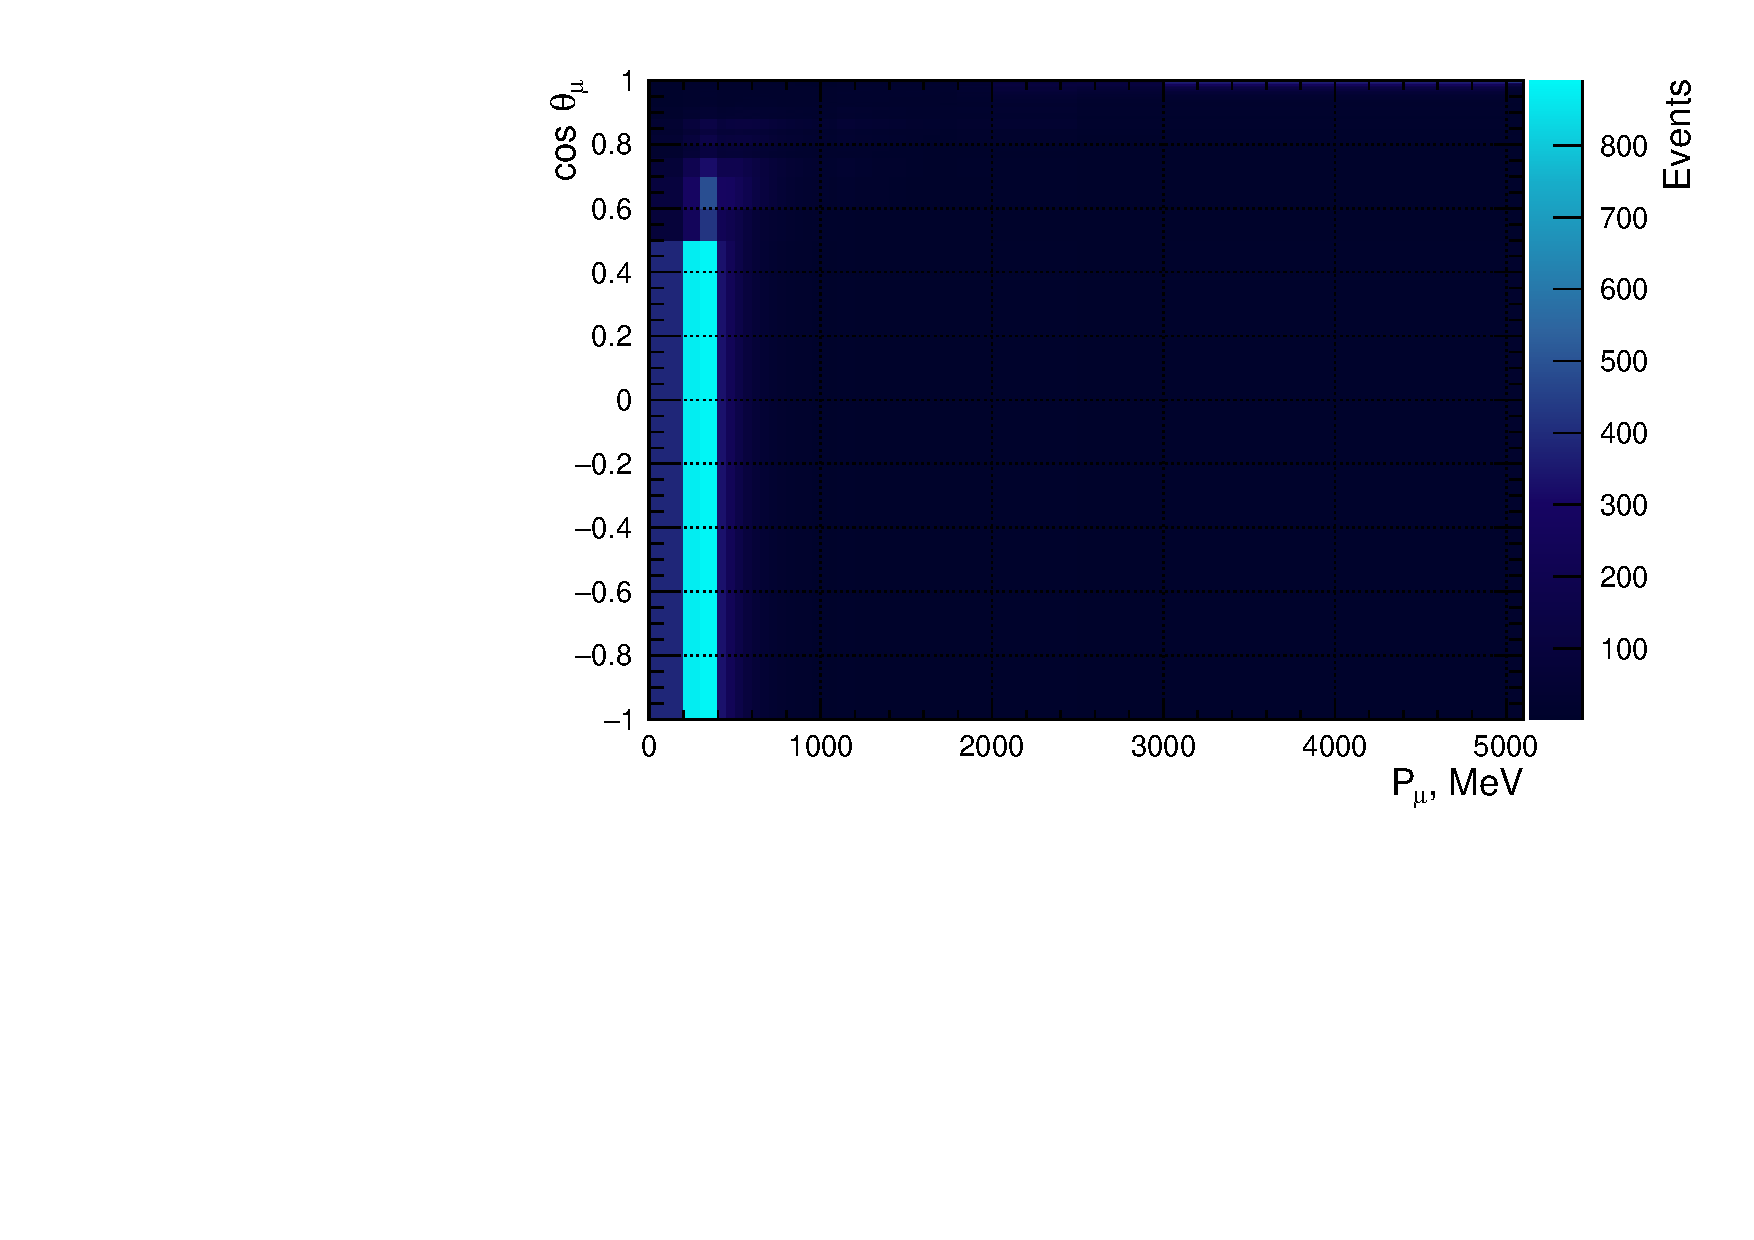
\includegraphics[width=0.95\linewidth]{figs/NomMC_MC_FGD2_numuCC_0pi}
  \caption{FGD2 FHC $\nu_{\mu}$ 0$\pi$}
  \label{fig:2d_FGD2_numuCC_0pi}
\end{subfigure}
\begin{subfigure}{.32\textwidth}
  \centering
  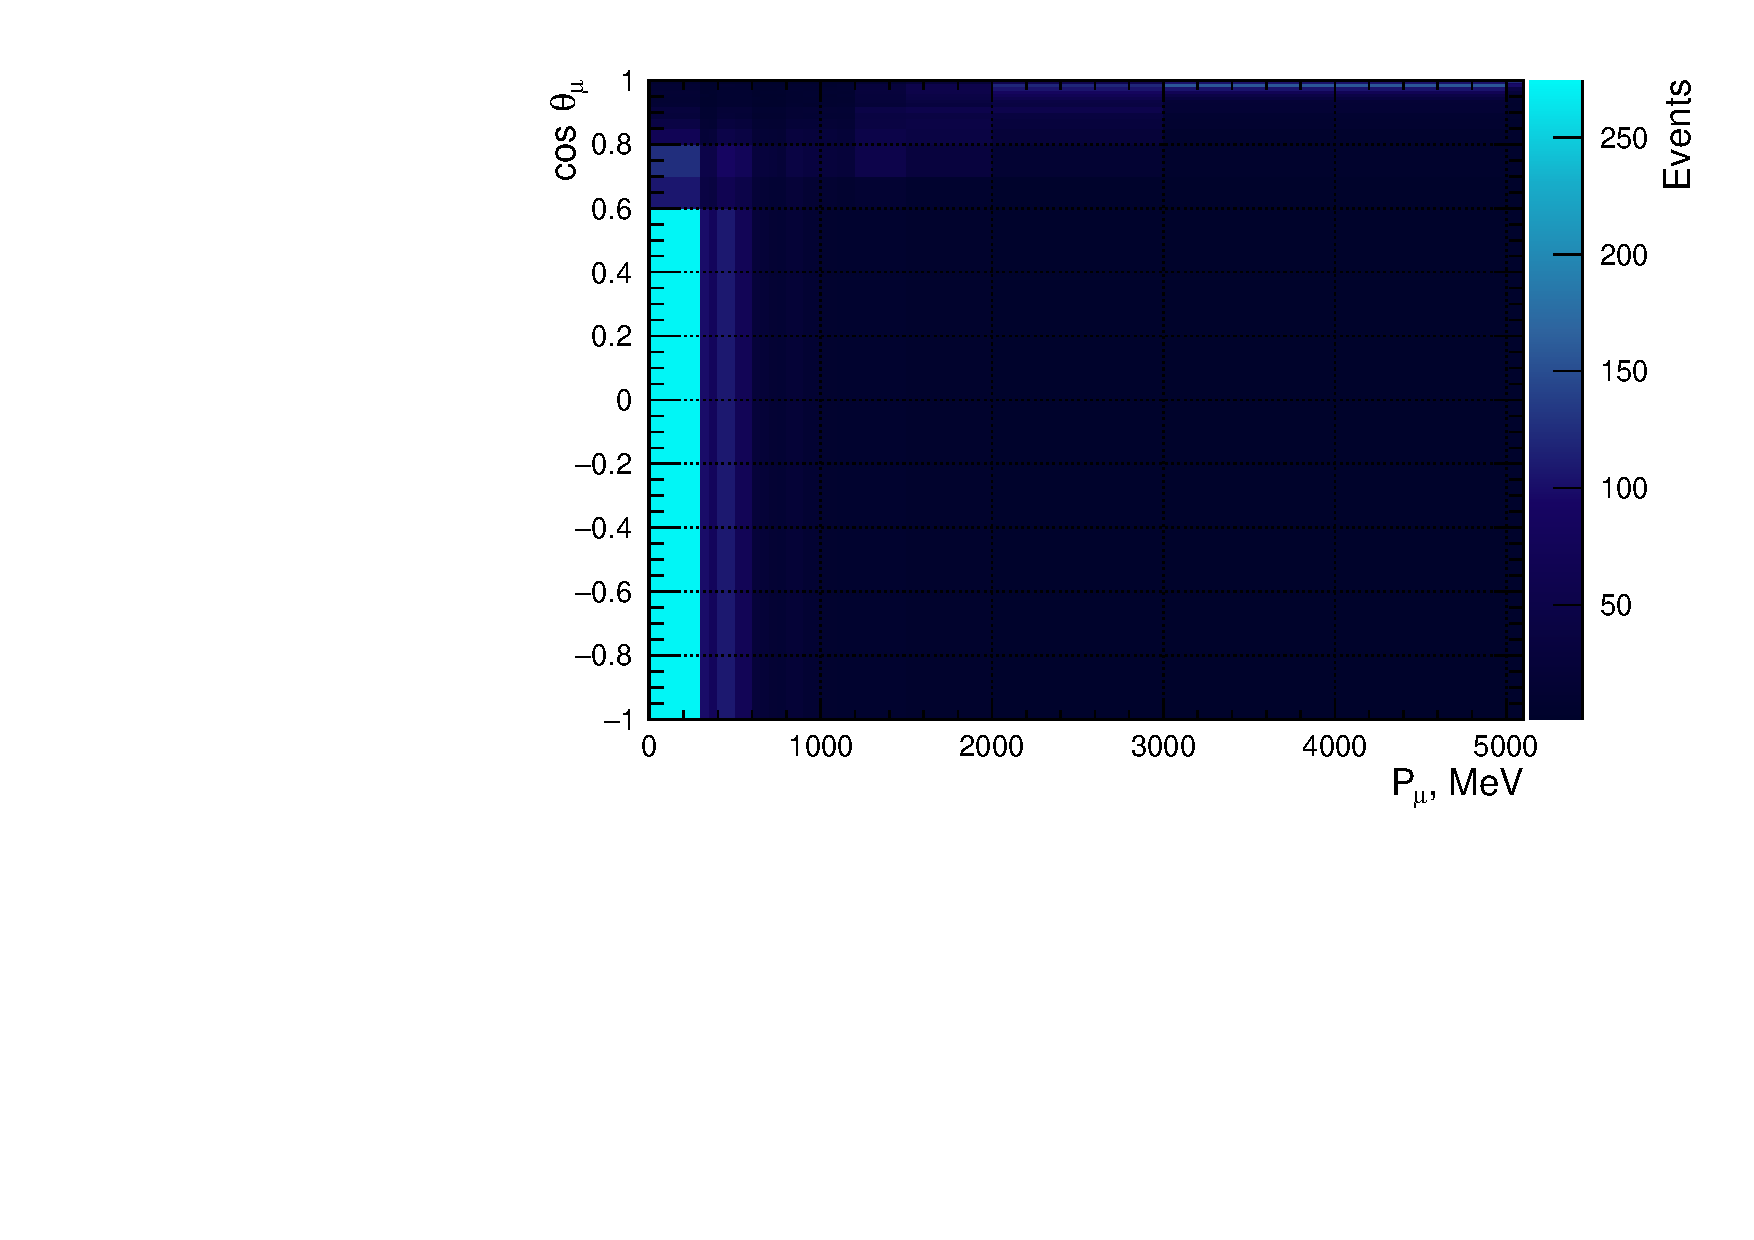
\includegraphics[width=0.95\linewidth]{figs/NomMC_MC_FGD2_numuCC_1pi}
  \caption{FGD2 FHC $\nu_{\mu}$ 1$\pi$}
  \label{fig:2d_FGD2_numuCC_1pi}
\end{subfigure}
\begin{subfigure}{.32\textwidth}
  \centering
  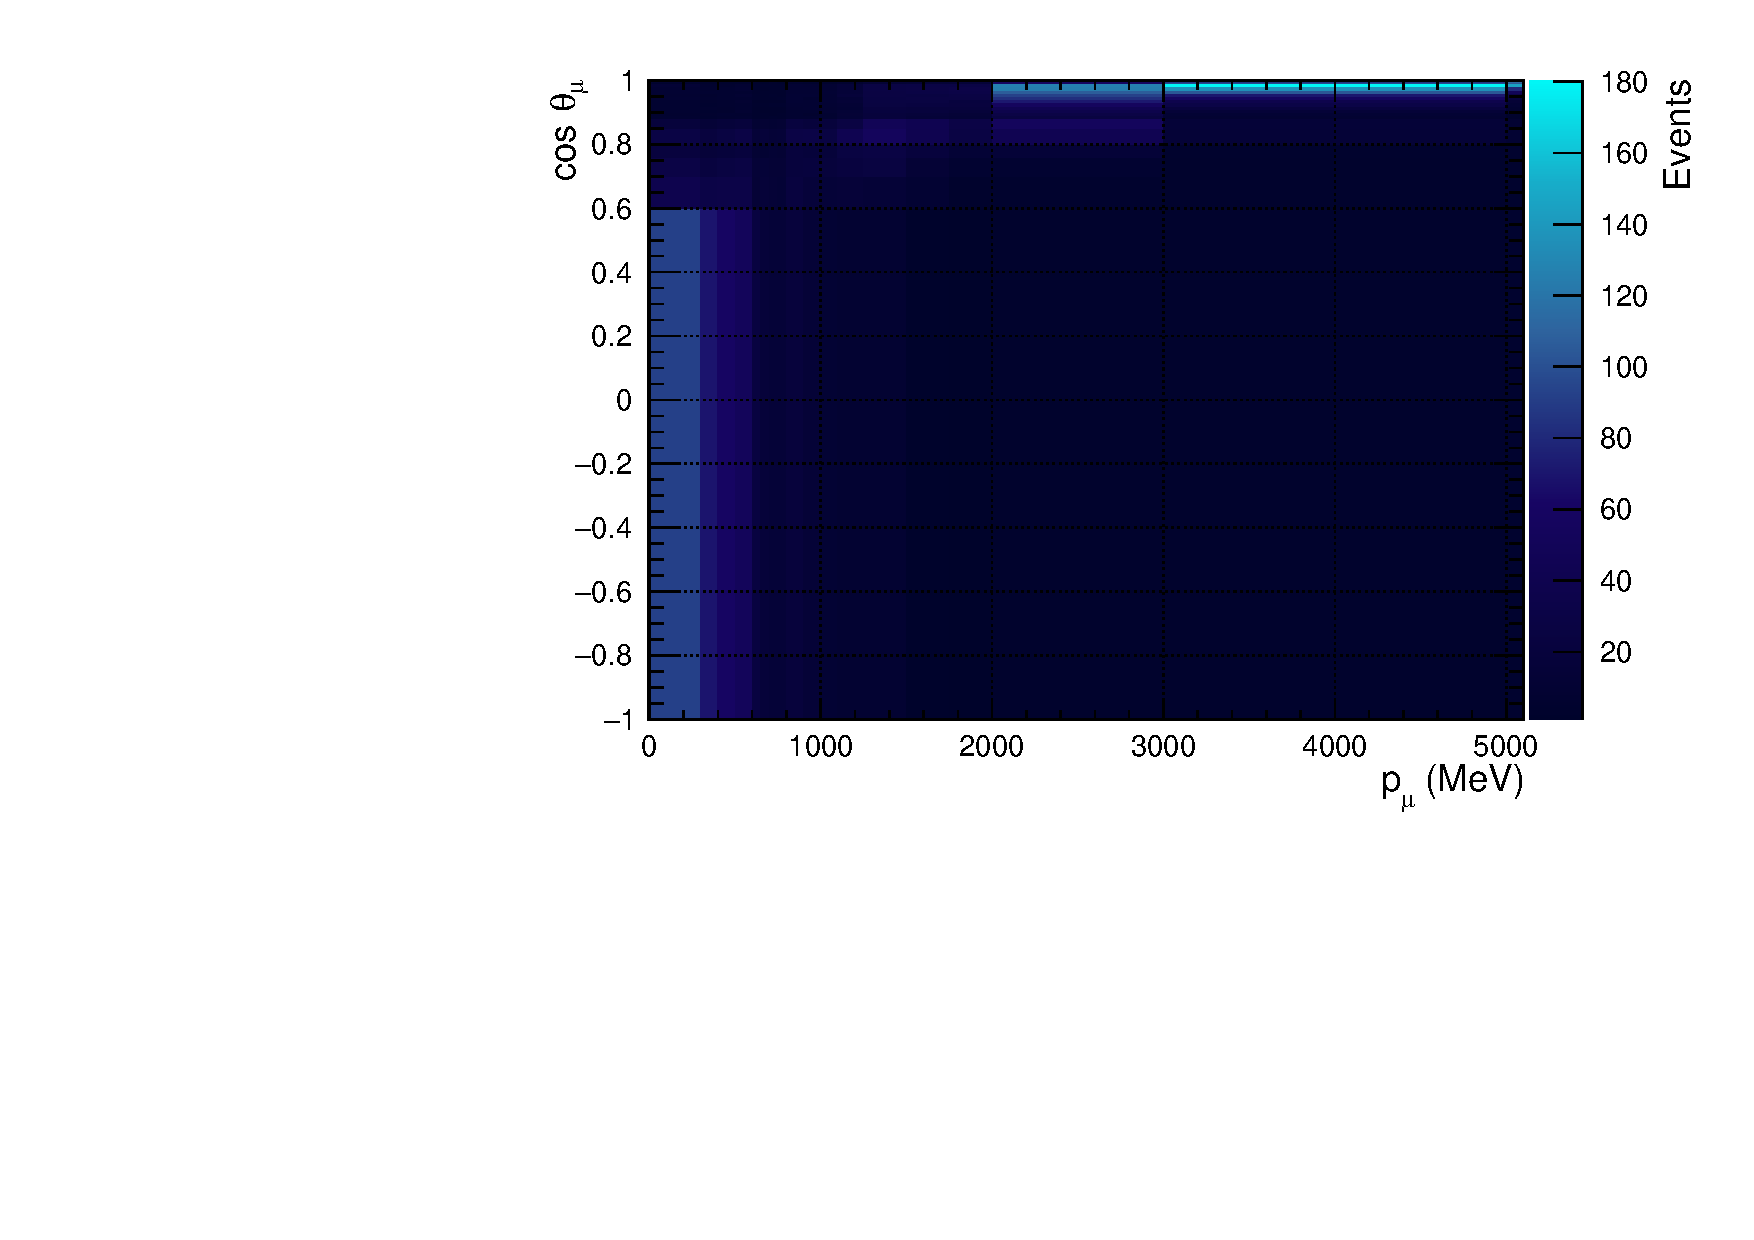
\includegraphics[width=0.95\linewidth]{figs/NomMC_MC_FGD2_numuCC_other}
  \caption{FGD2 FHC $\nu_{\mu}$ Other}
  \label{fig:2d_FGD2_numuCC_other}
\end{subfigure}
\centering
\begin{subfigure}{.32\textwidth}
  \centering
  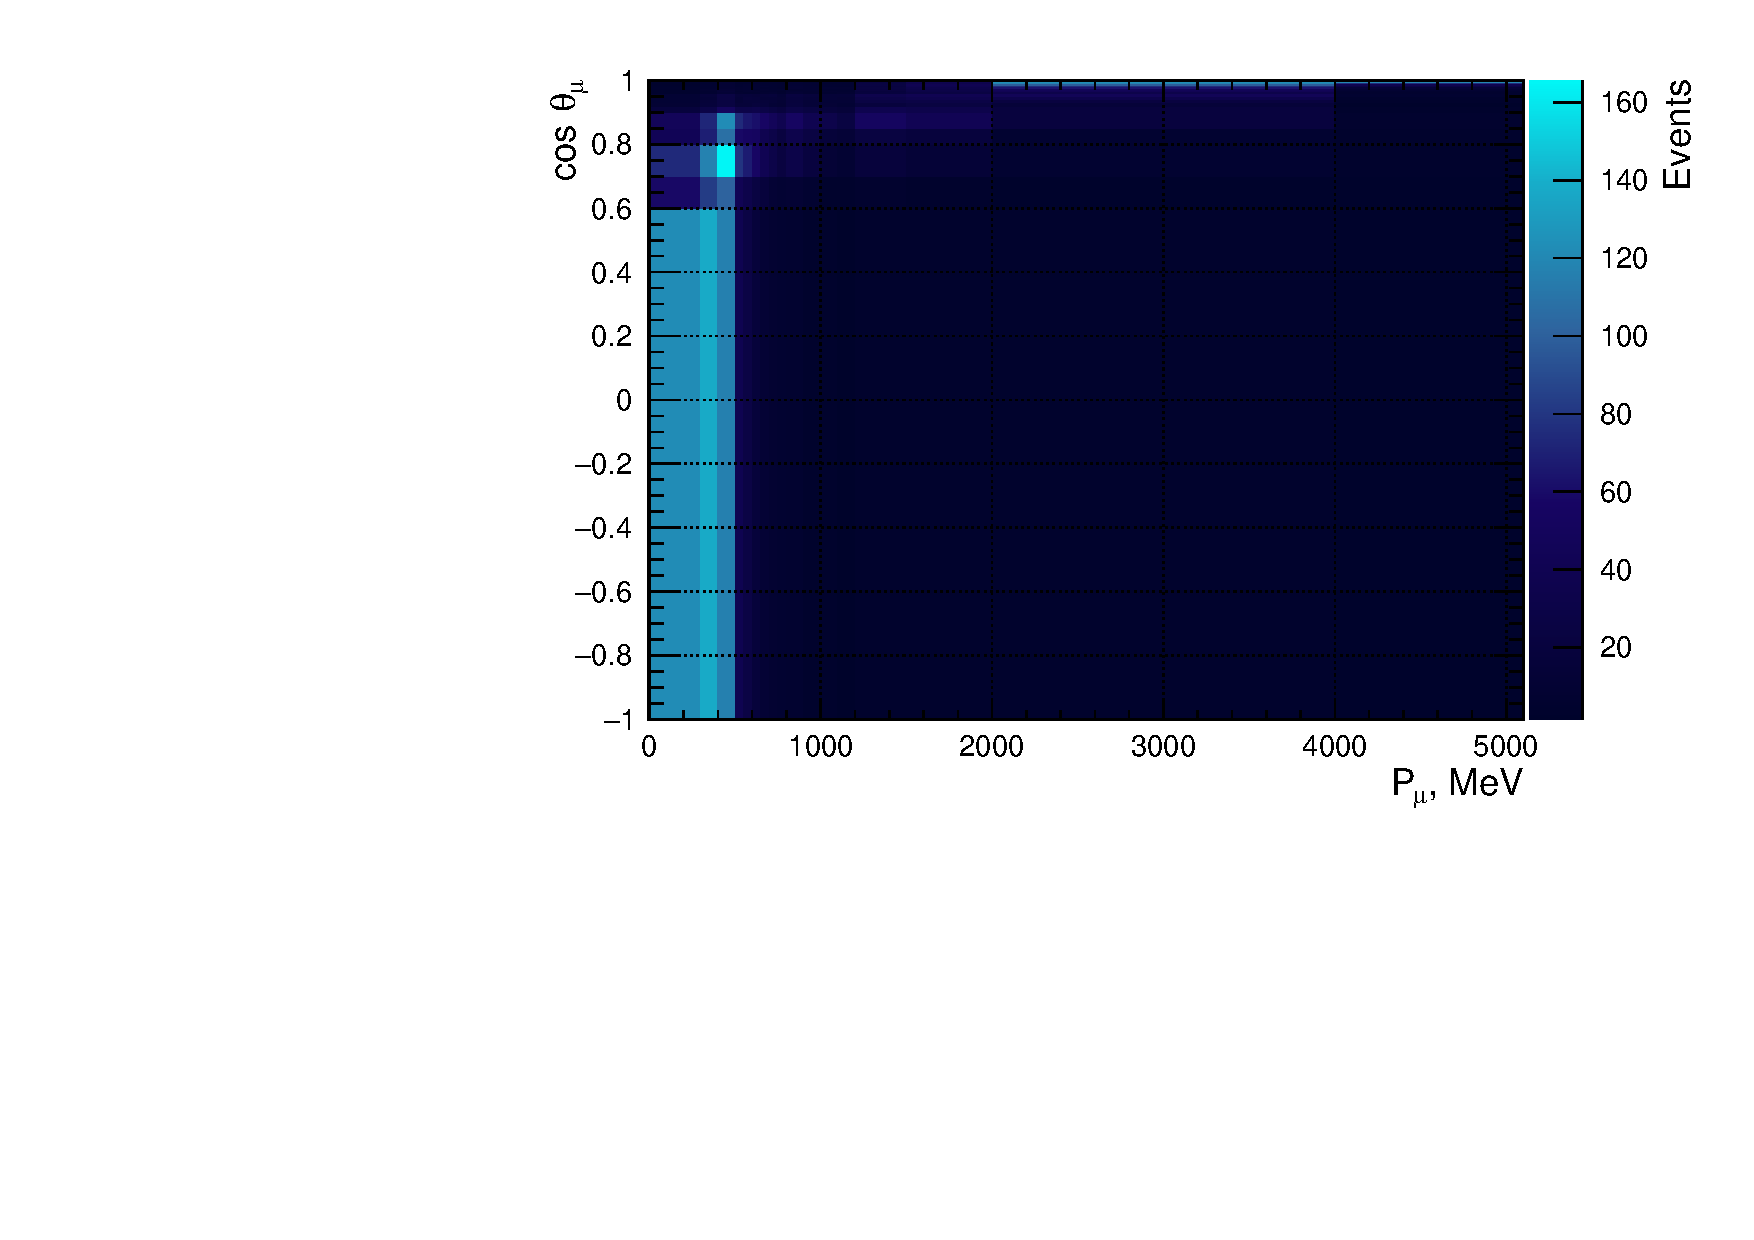
\includegraphics[width=0.95\linewidth]{figs/NomMC_MC_FGD1_anti-numuCC_0pi}
  \caption{FGD1 RHC $\bar{\nu_{\mu}}$ 0$\pi$}
  \label{fig:2d_FGD1_anti-numuCC_0pi}
\end{subfigure}
\begin{subfigure}{.32\textwidth}
  \centering
  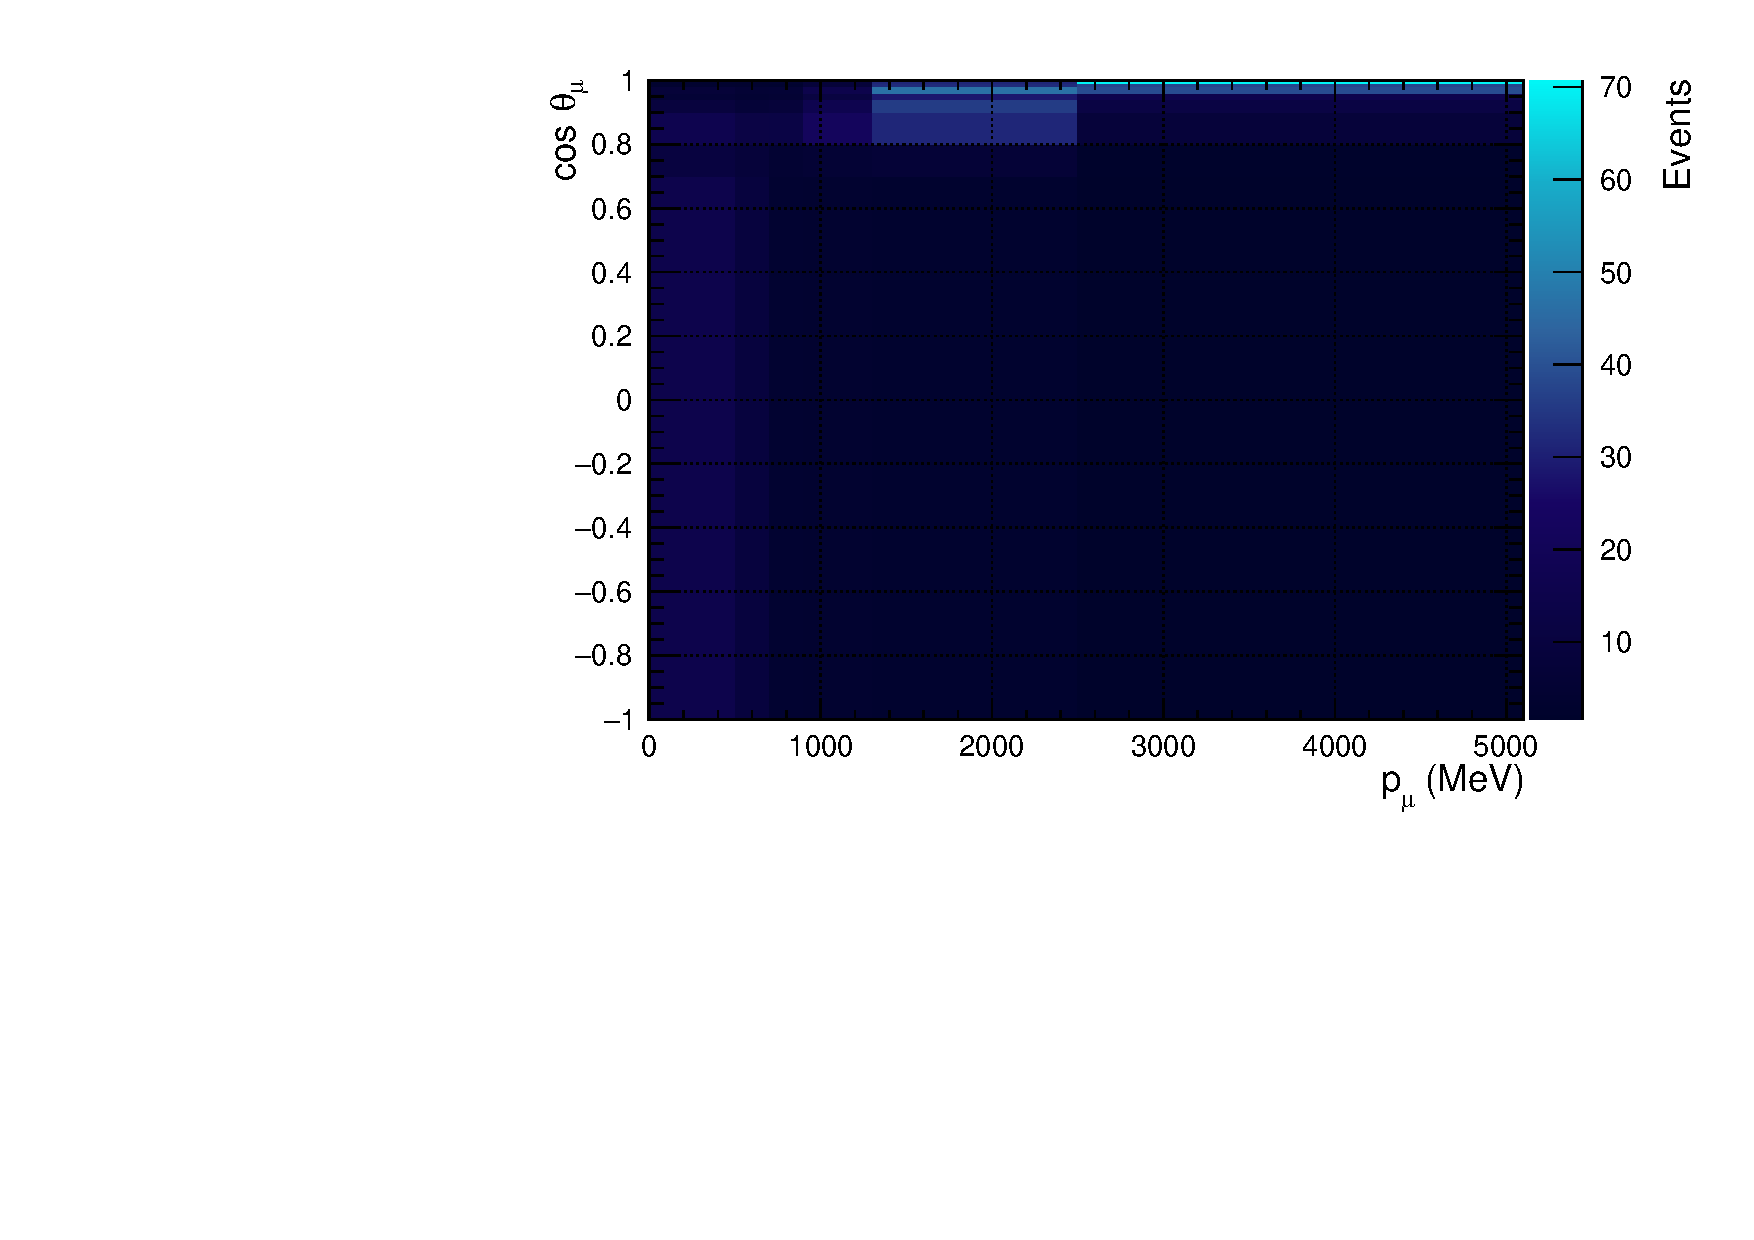
\includegraphics[width=0.95\linewidth]{figs/NomMC_MC_FGD1_anti-numuCC_1pi}
  \caption{FGD1 RHC $\bar{\nu_{\mu}}$ 1$\pi$}
  \label{fig:2d_FGD1_anti-numuCC_1pi}
\end{subfigure}
\begin{subfigure}{.32\textwidth}
  \centering
  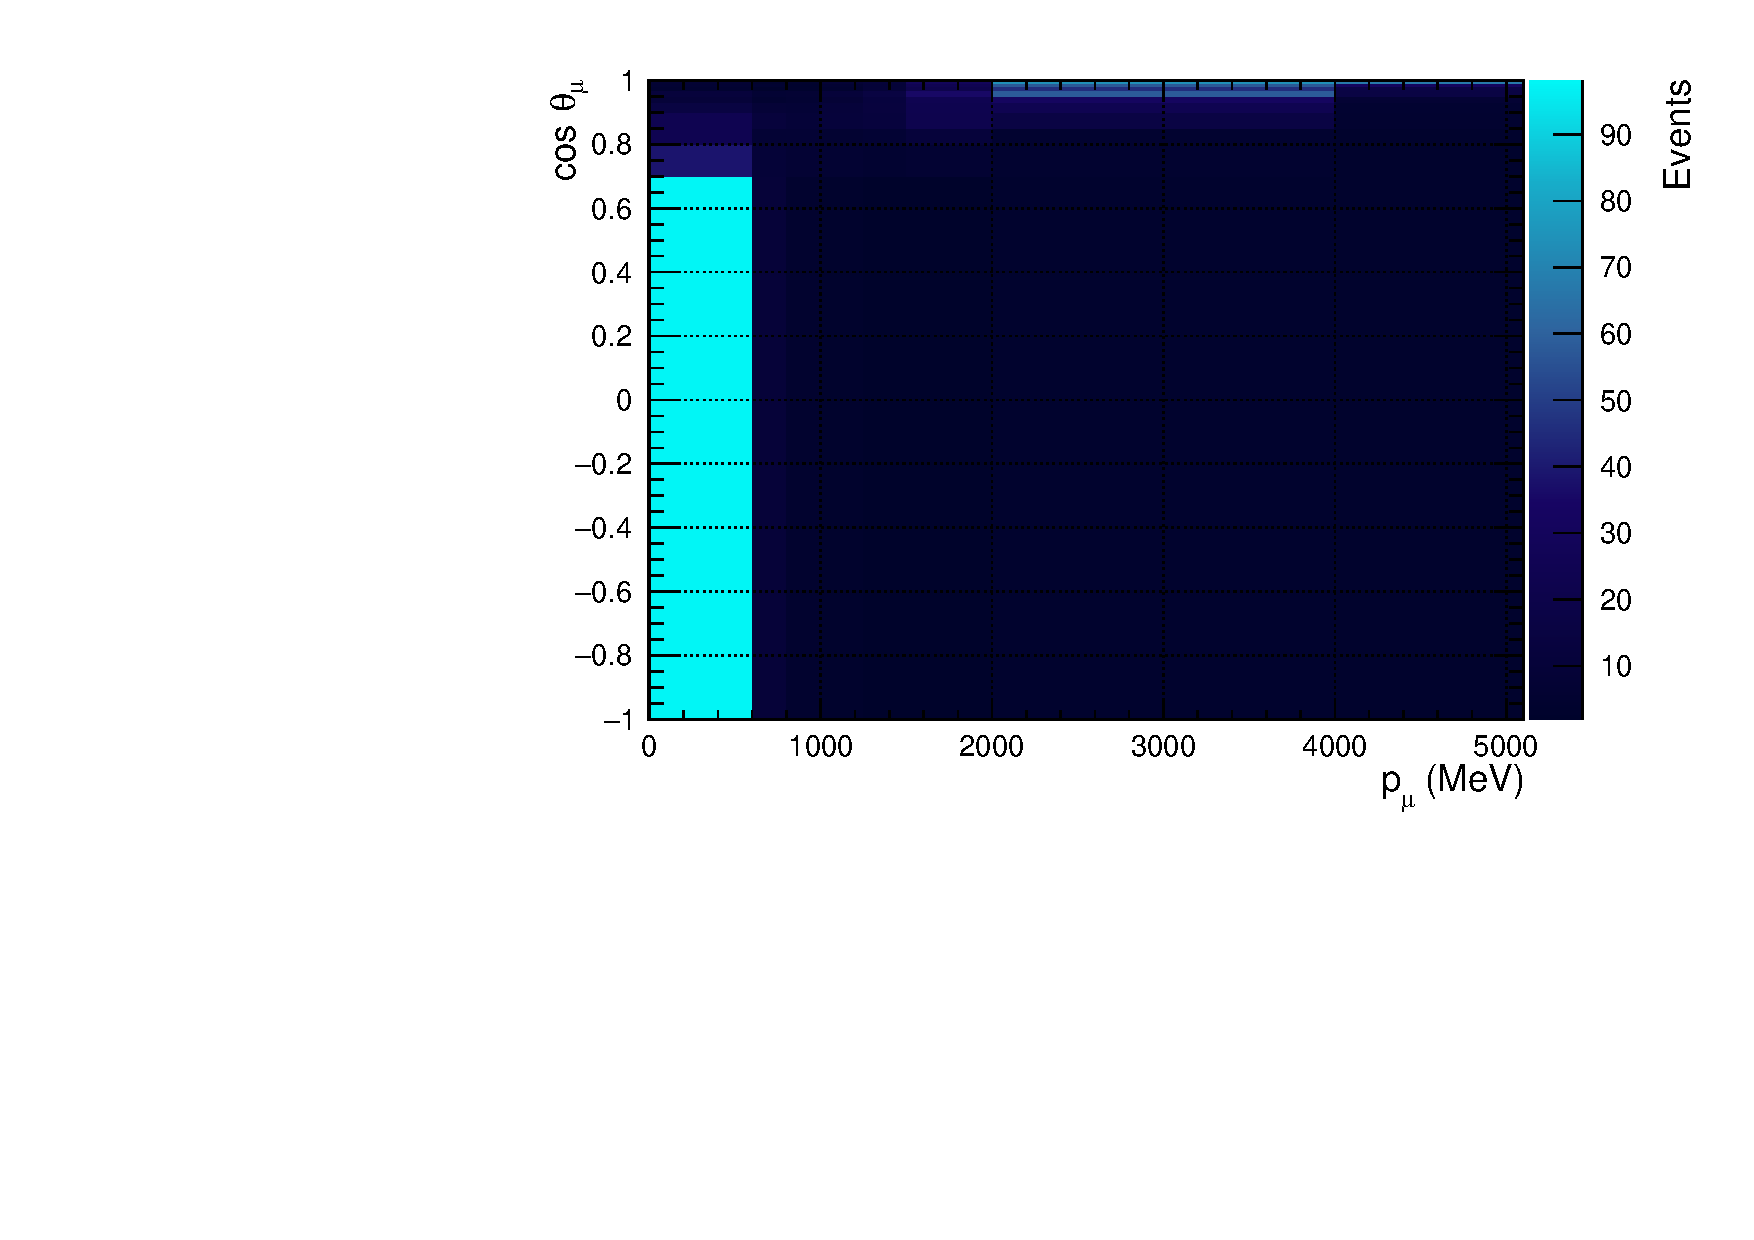
\includegraphics[width=0.95\linewidth]{figs/NomMC_MC_FGD1_anti-numuCC_other}
  \caption{FGD1 RHC $\bar{\nu_{\mu}}$ Other}
  \label{fig:2d_FGD1_anti-numuCC_other}
\end{subfigure}
\centering
\begin{subfigure}{.32\textwidth}
  \centering
  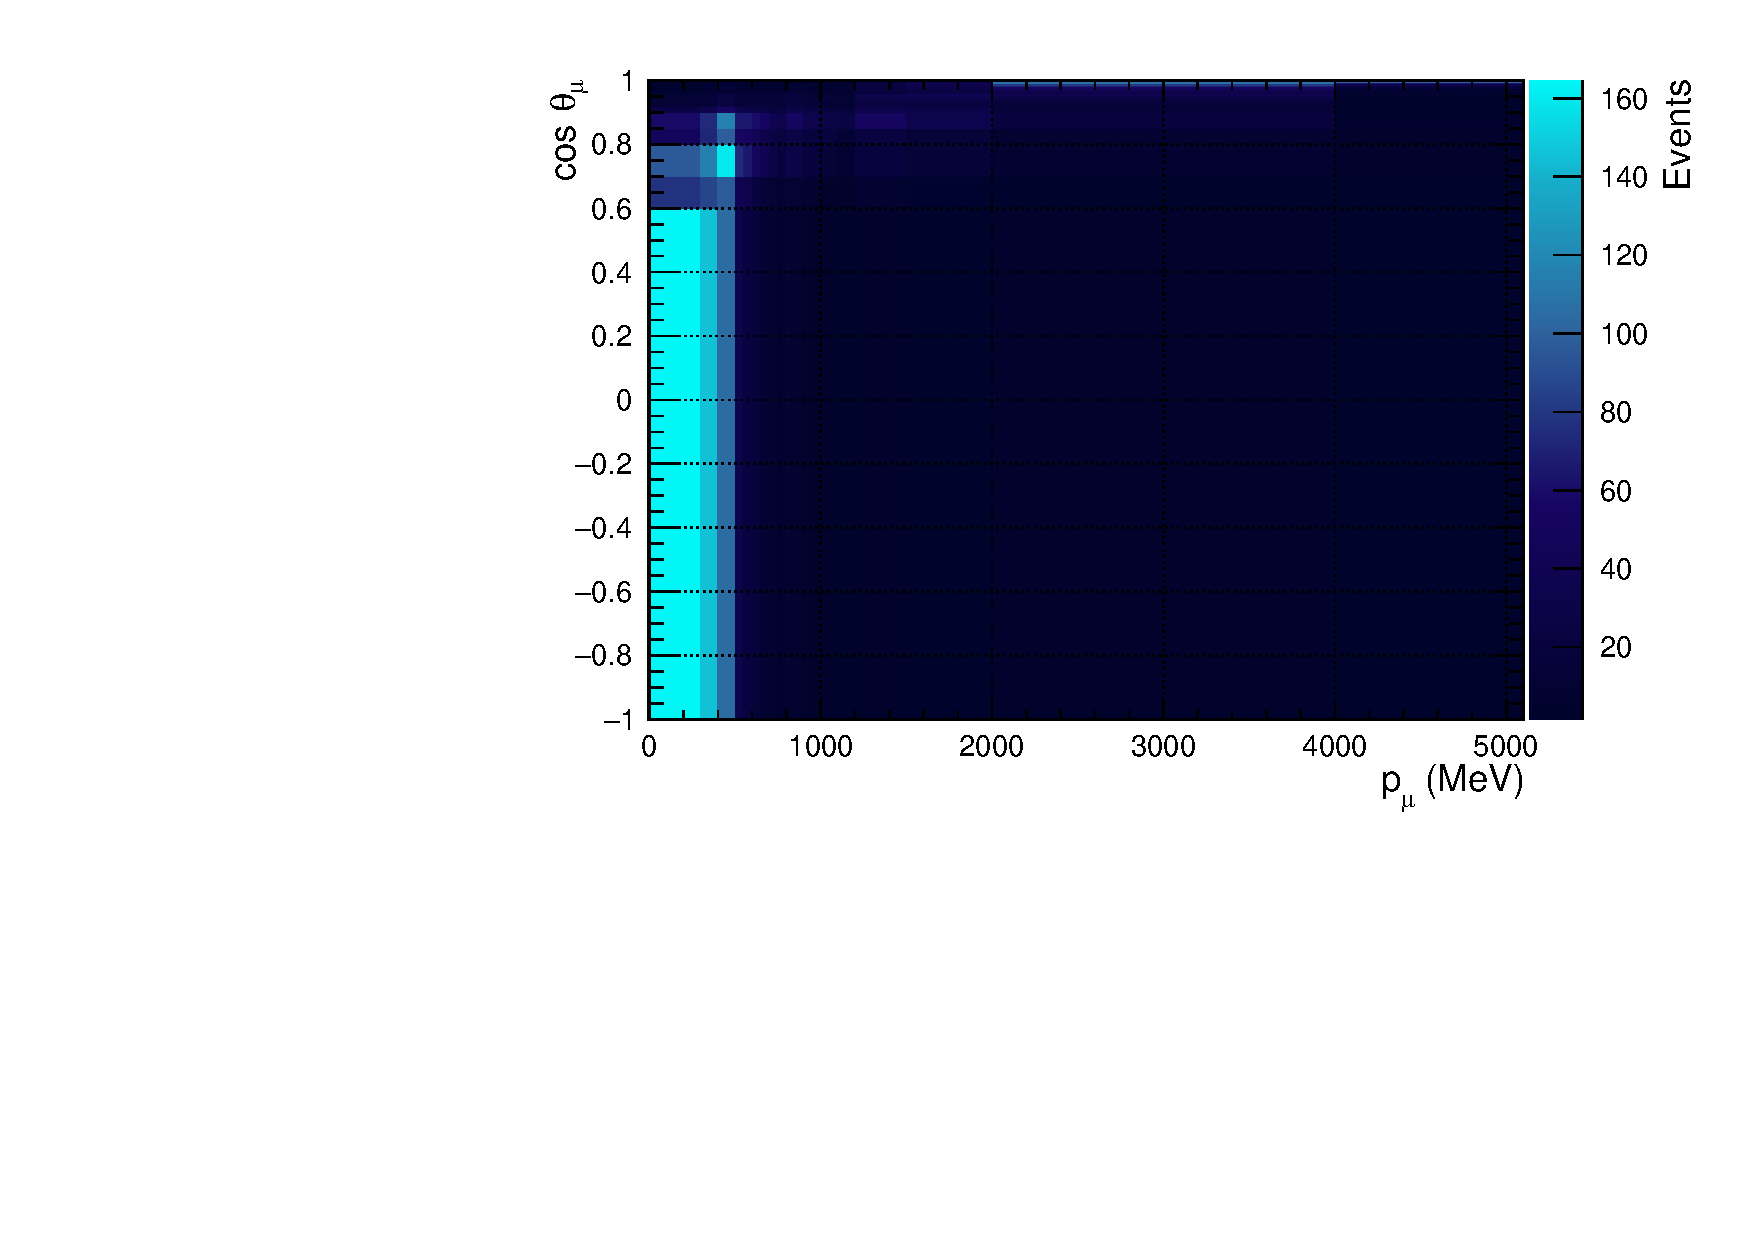
\includegraphics[width=0.95\linewidth]{figs/NomMC_MC_FGD2_anti-numuCC_0pi}
  \caption{FGD2 RHC $\bar{\nu_{\mu}}$ 0$\pi$}
  \label{fig:2d_FGD2_anti-numuCC_0pi}
\end{subfigure}
\begin{subfigure}{.32\textwidth}
  \centering
  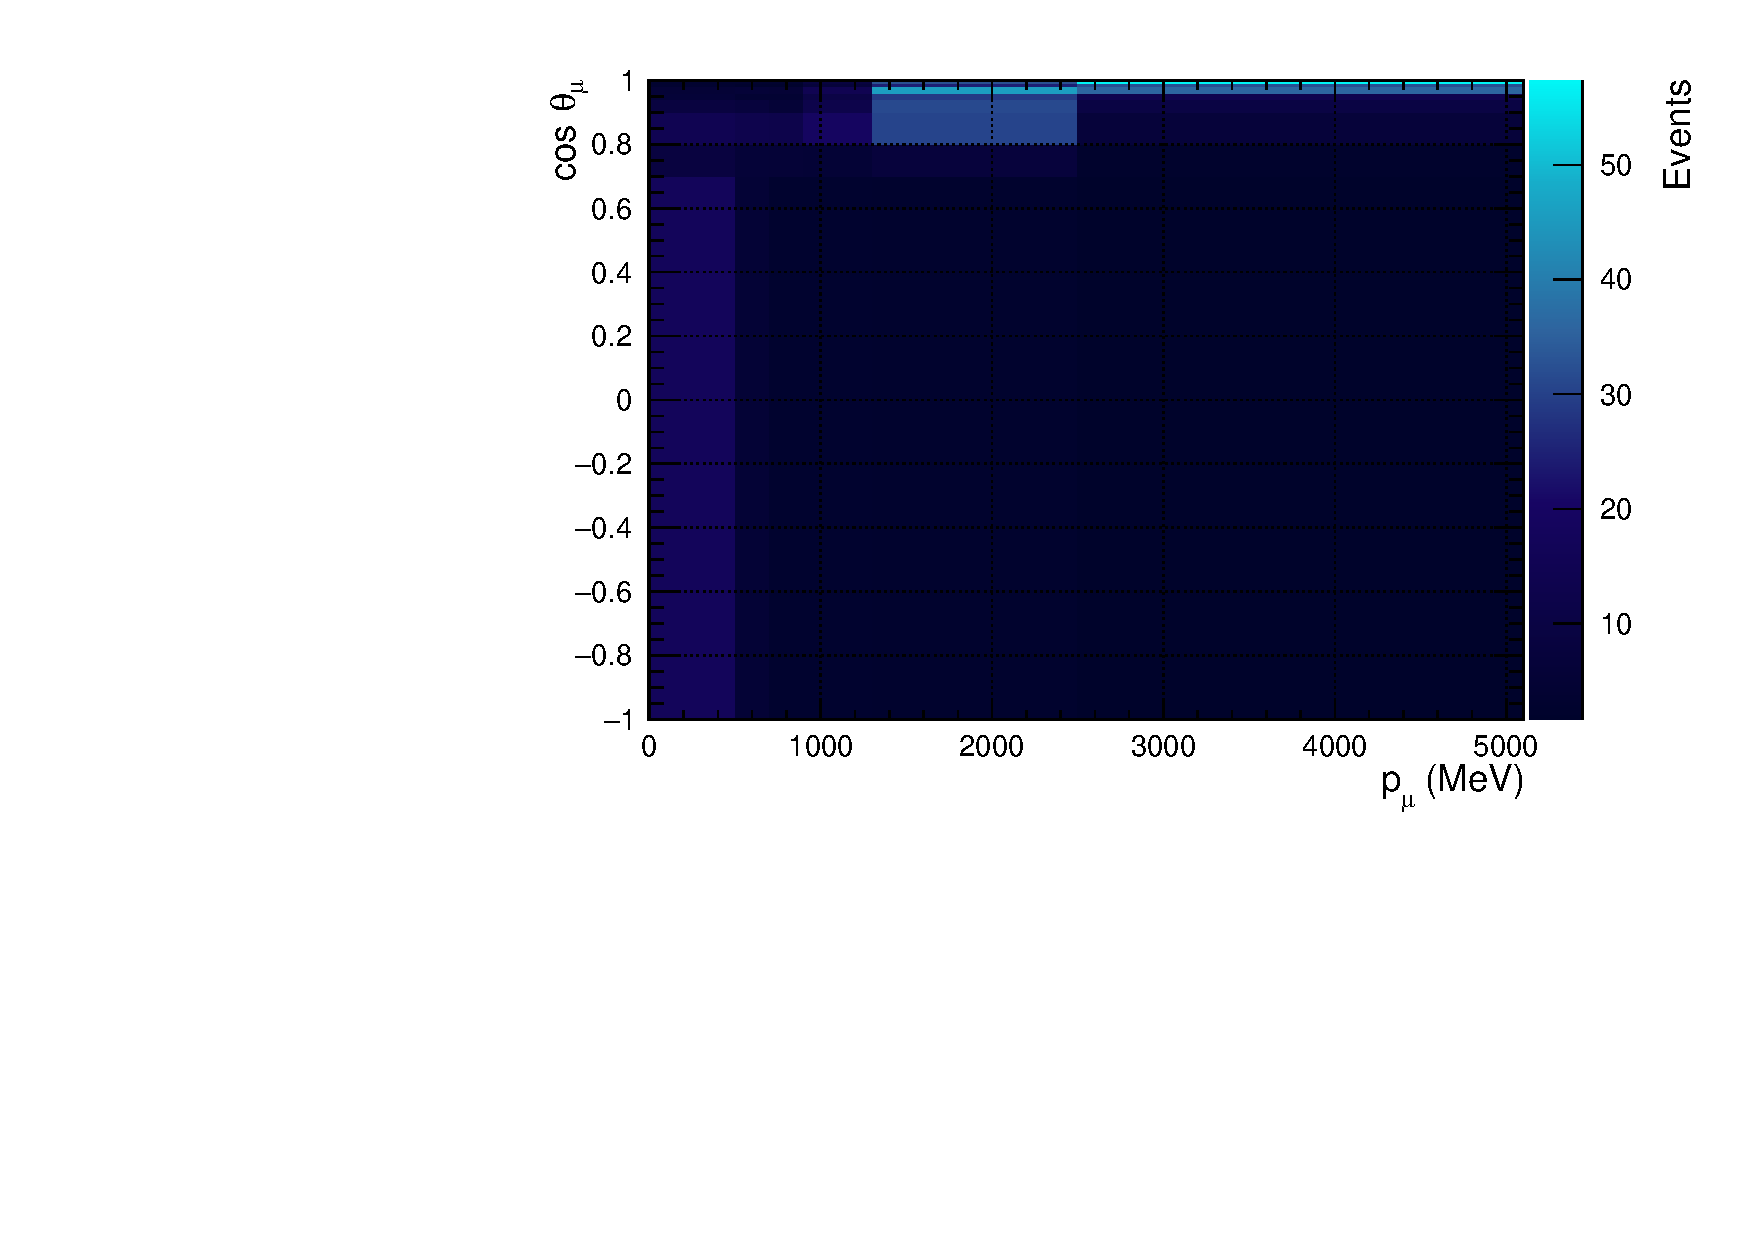
\includegraphics[width=0.95\linewidth]{figs/NomMC_MC_FGD2_anti-numuCC_1pi}
  \caption{FGD2 RHC $\bar{\nu_{\mu}}$ 1$\pi$}
  \label{fig:2d_FGD2_anti-numuCC_1pi}
\end{subfigure}
\begin{subfigure}{.32\textwidth}
  \centering
  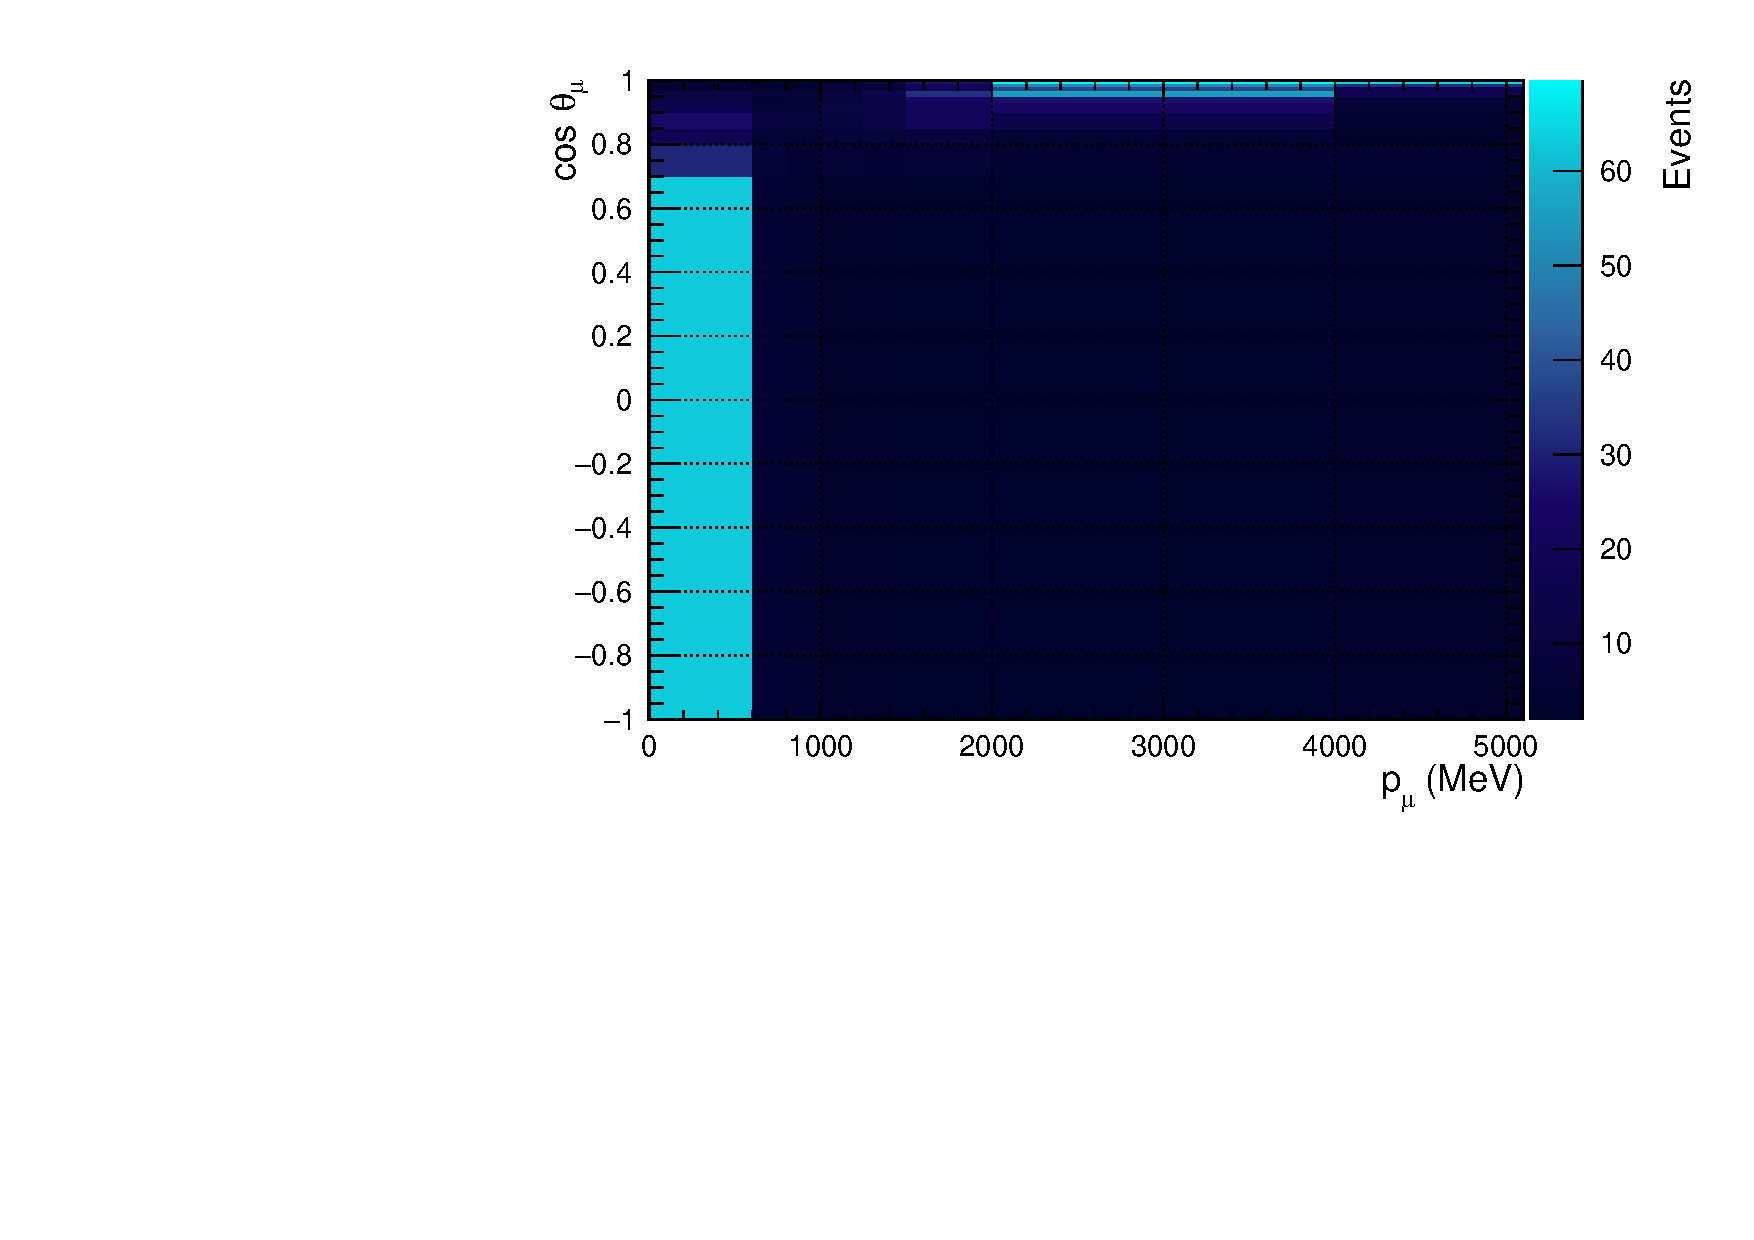
\includegraphics[width=0.95\linewidth]{figs/NomMC_MC_FGD2_anti-numuCC_other}
  \caption{FGD2 RHC $\bar{\nu_{\mu}}$ Other}
  \label{fig:2d_FGD2_anti-numuCC_other}
\end{subfigure}
\begin{subfigure}{.32\textwidth}
  \centering
  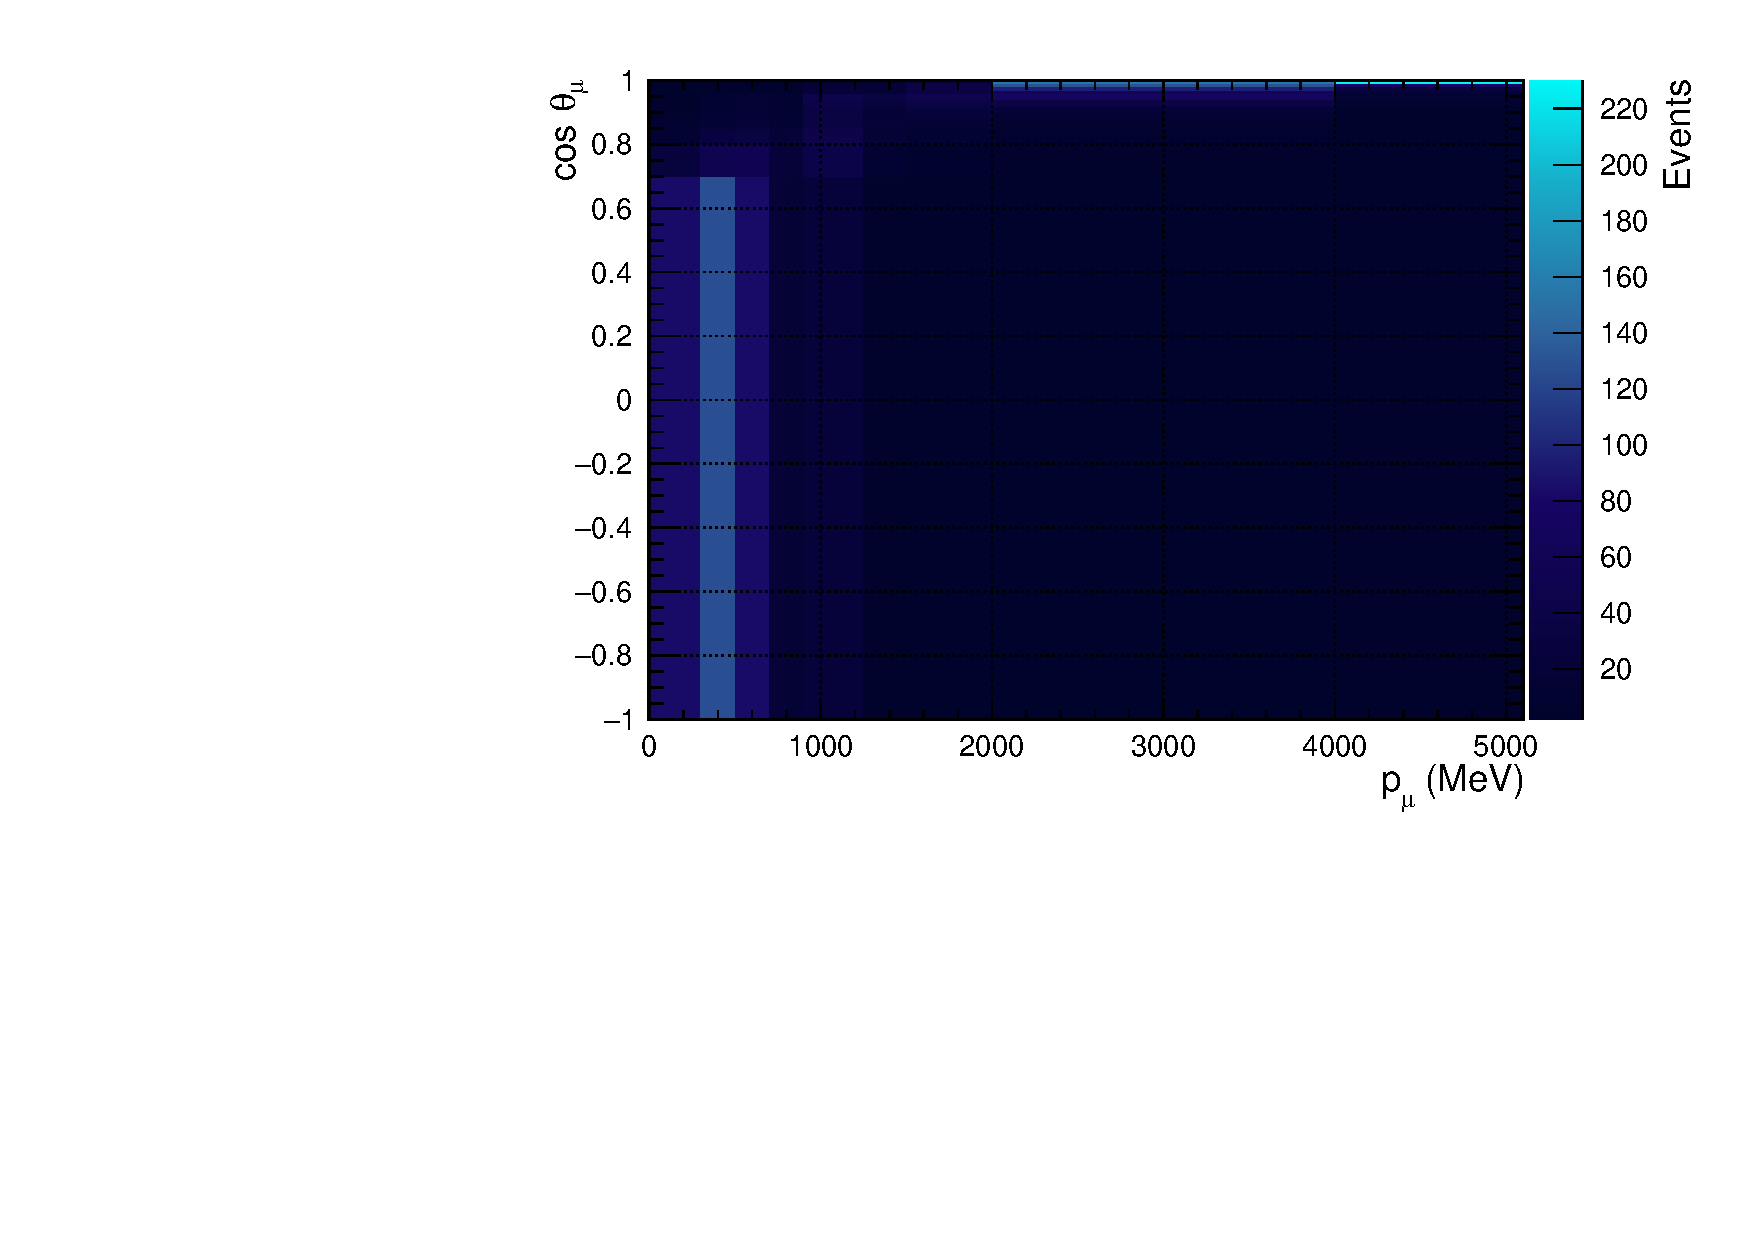
\includegraphics[width=0.95\linewidth]{figs/NomMC_MC_FGD1_NuMuBkg_CC0pi_in_AntiNu_Mode}
  \caption{FGD1 RHC $\nu_{\mu}$ 0$\pi$}
  \label{fig:2d_FGD1_NuMuBkg_CC0pi_in_AntiNu_Mode}
\end{subfigure}
\begin{subfigure}{.32\textwidth}
  \centering
  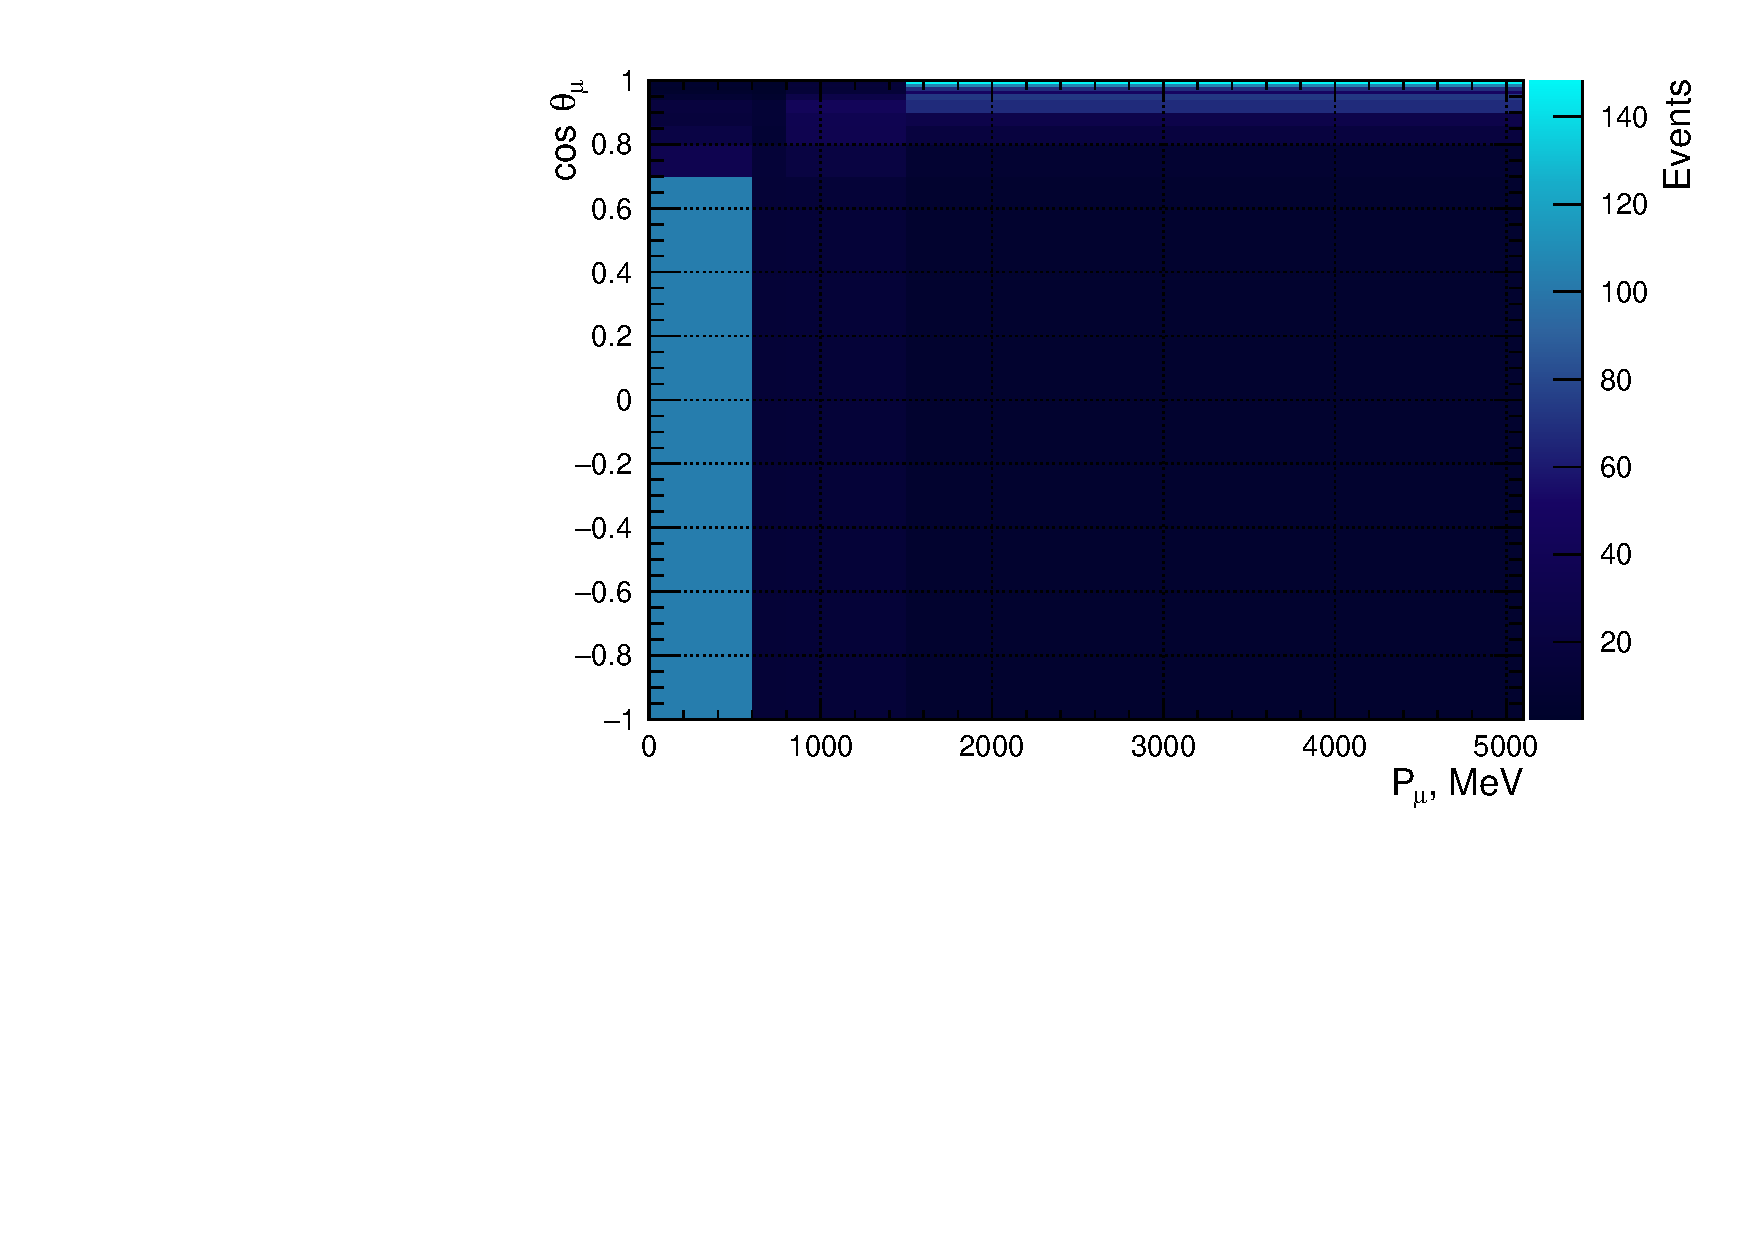
\includegraphics[width=0.95\linewidth]{figs/NomMC_MC_FGD1_NuMuBkg_CC1pi_in_AntiNu_Mode}
  \caption{FGD1 RHC $\nu_{\mu}$ 1$\pi$}
  \label{fig:2d_FGD1_NuMuBkg_CC1pi_in_AntiNu_Mode}
\end{subfigure}
\begin{subfigure}{.32\textwidth}
  \centering
  \includegraphics[width=0.95\linewidth]{figs/NomMC_MC_FGD1_NuMuBkg_CCOther_in_AntiNu_Mode}
  \caption{FGD1 RHC $\nu_{\mu}$ Other}
  \label{fig:2d_FGD1_NuMuBkg_CCOther_in_AntiNu_Mode}
\end{subfigure}
\begin{subfigure}{.32\textwidth}
  \centering
  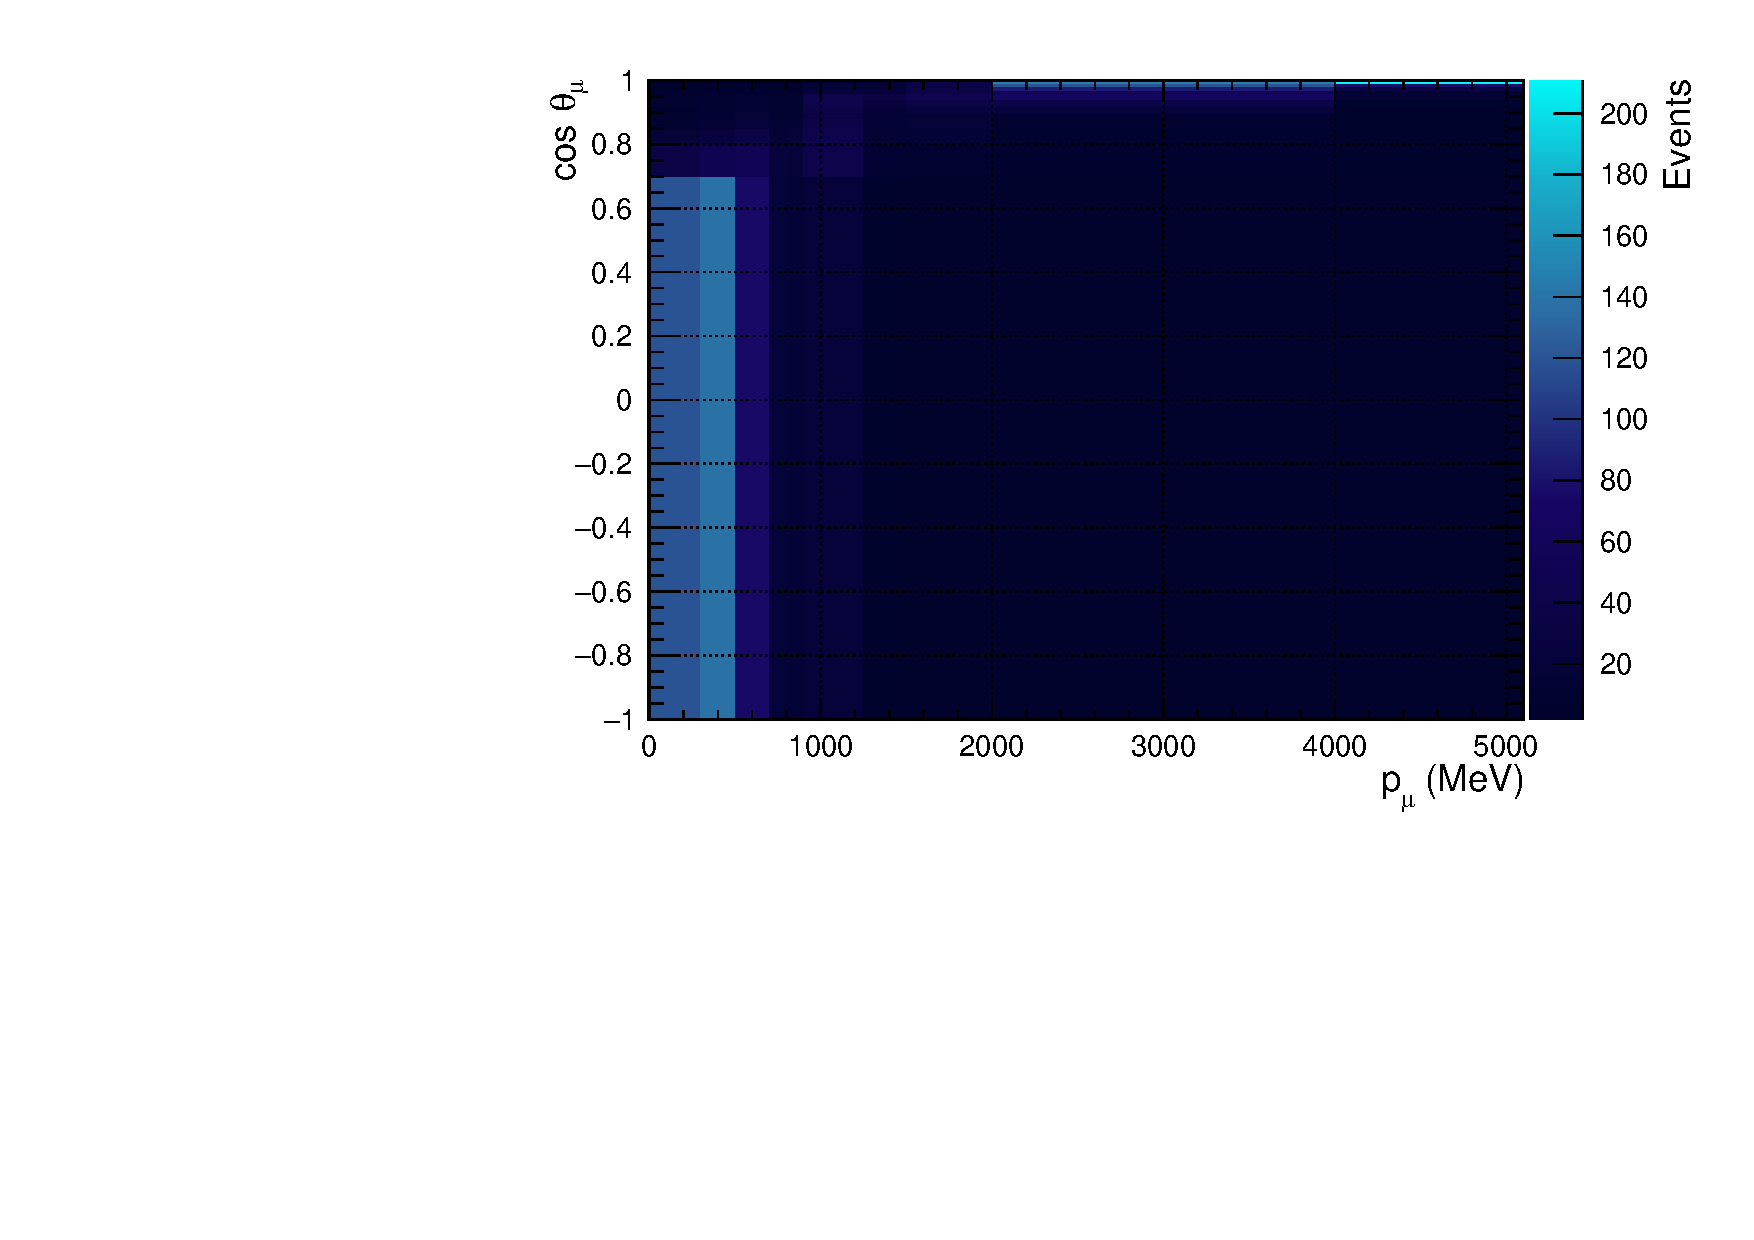
\includegraphics[width=0.95\linewidth]{figs/NomMC_MC_FGD2_NuMuBkg_CC0pi_in_AntiNu_Mode}
  \caption{FGD2 RHC $\nu_{\mu}$ 0$\pi$}
  \label{fig:2d_FGD2_NuMuBkg_CC0pi_in_AntiNu_Mode}
\end{subfigure}
\begin{subfigure}{.32\textwidth}
  \centering
  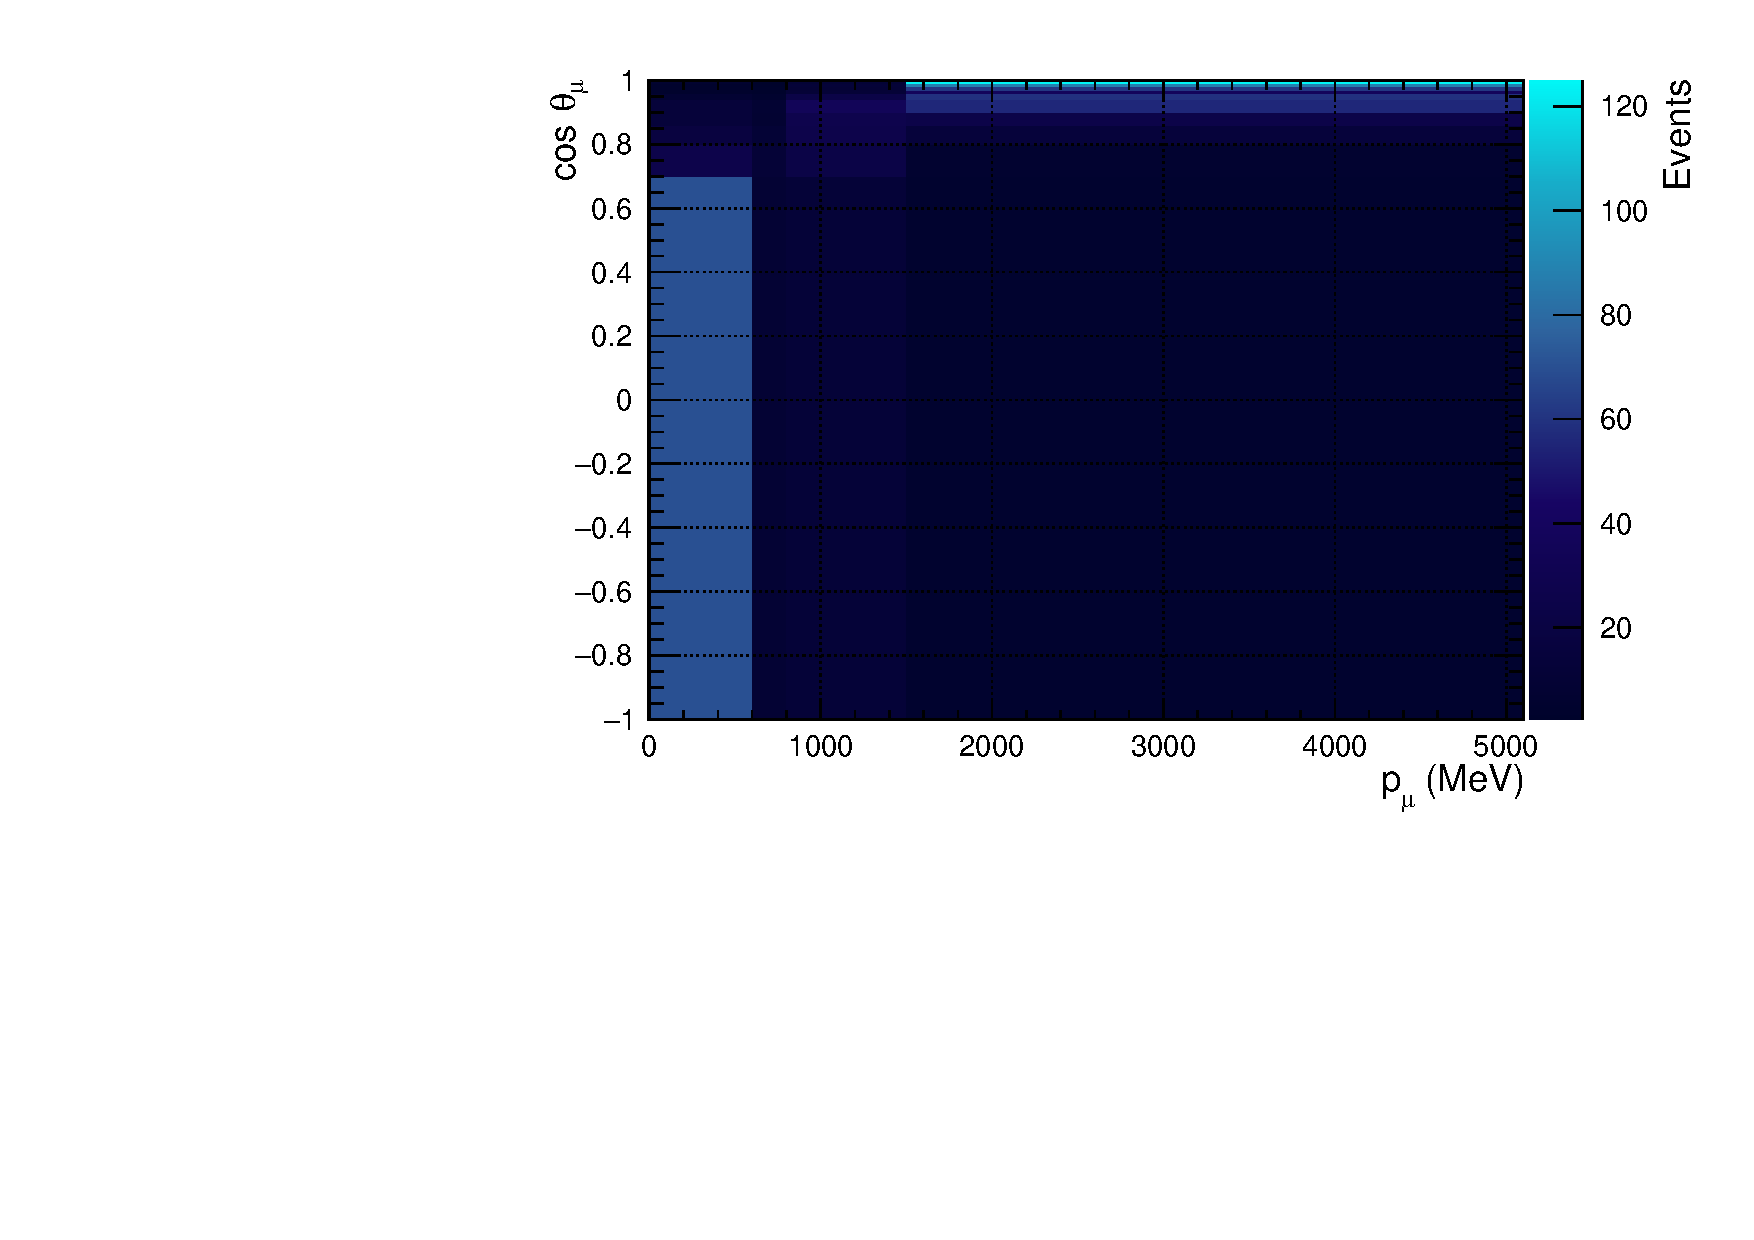
\includegraphics[width=0.95\linewidth]{figs/NomMC_MC_FGD2_NuMuBkg_CC1pi_in_AntiNu_Mode}
  \caption{FGD2 RHC $\nu_{\mu}$ 1$\pi$}
  \label{fig:2d_FGD2_NuMuBkg_CC1pi_in_AntiNu_Mode}
\end{subfigure}
\begin{subfigure}{.32\textwidth}
  \centering
  \includegraphics[width=0.95\linewidth]{figs/NomMC_MC_FGD2_NuMuBkg_CCOther_in_AntiNu_Mode}
  \caption{FGD2 RHC $\nu_{\mu}$ Other}
  \label{fig:2d_FGD2_NuMuBkg_CCOther_in_AntiNu_Mode}
\end{subfigure}
\caption{$p_{\mu}$--cos$\theta_{\mu}$ distributions for the nominal MC binned uniformly.}
\label{fig:2dnomall}
\end{figure}

The projection of the non-uniformly binned nominal MC distributions onto the $p_{\mu}$ axis are shown in Figures \ref{fig:pstack_fhcapp}, \ref{fig:pstack_rhc_numubapp}, and \ref{fig:pstack_rhc_numuapp}, along with the interaction mode breakdown and data.

\begin{figure}[!t]
\centering
\begin{subfigure}{.24\textwidth}
  \centering
  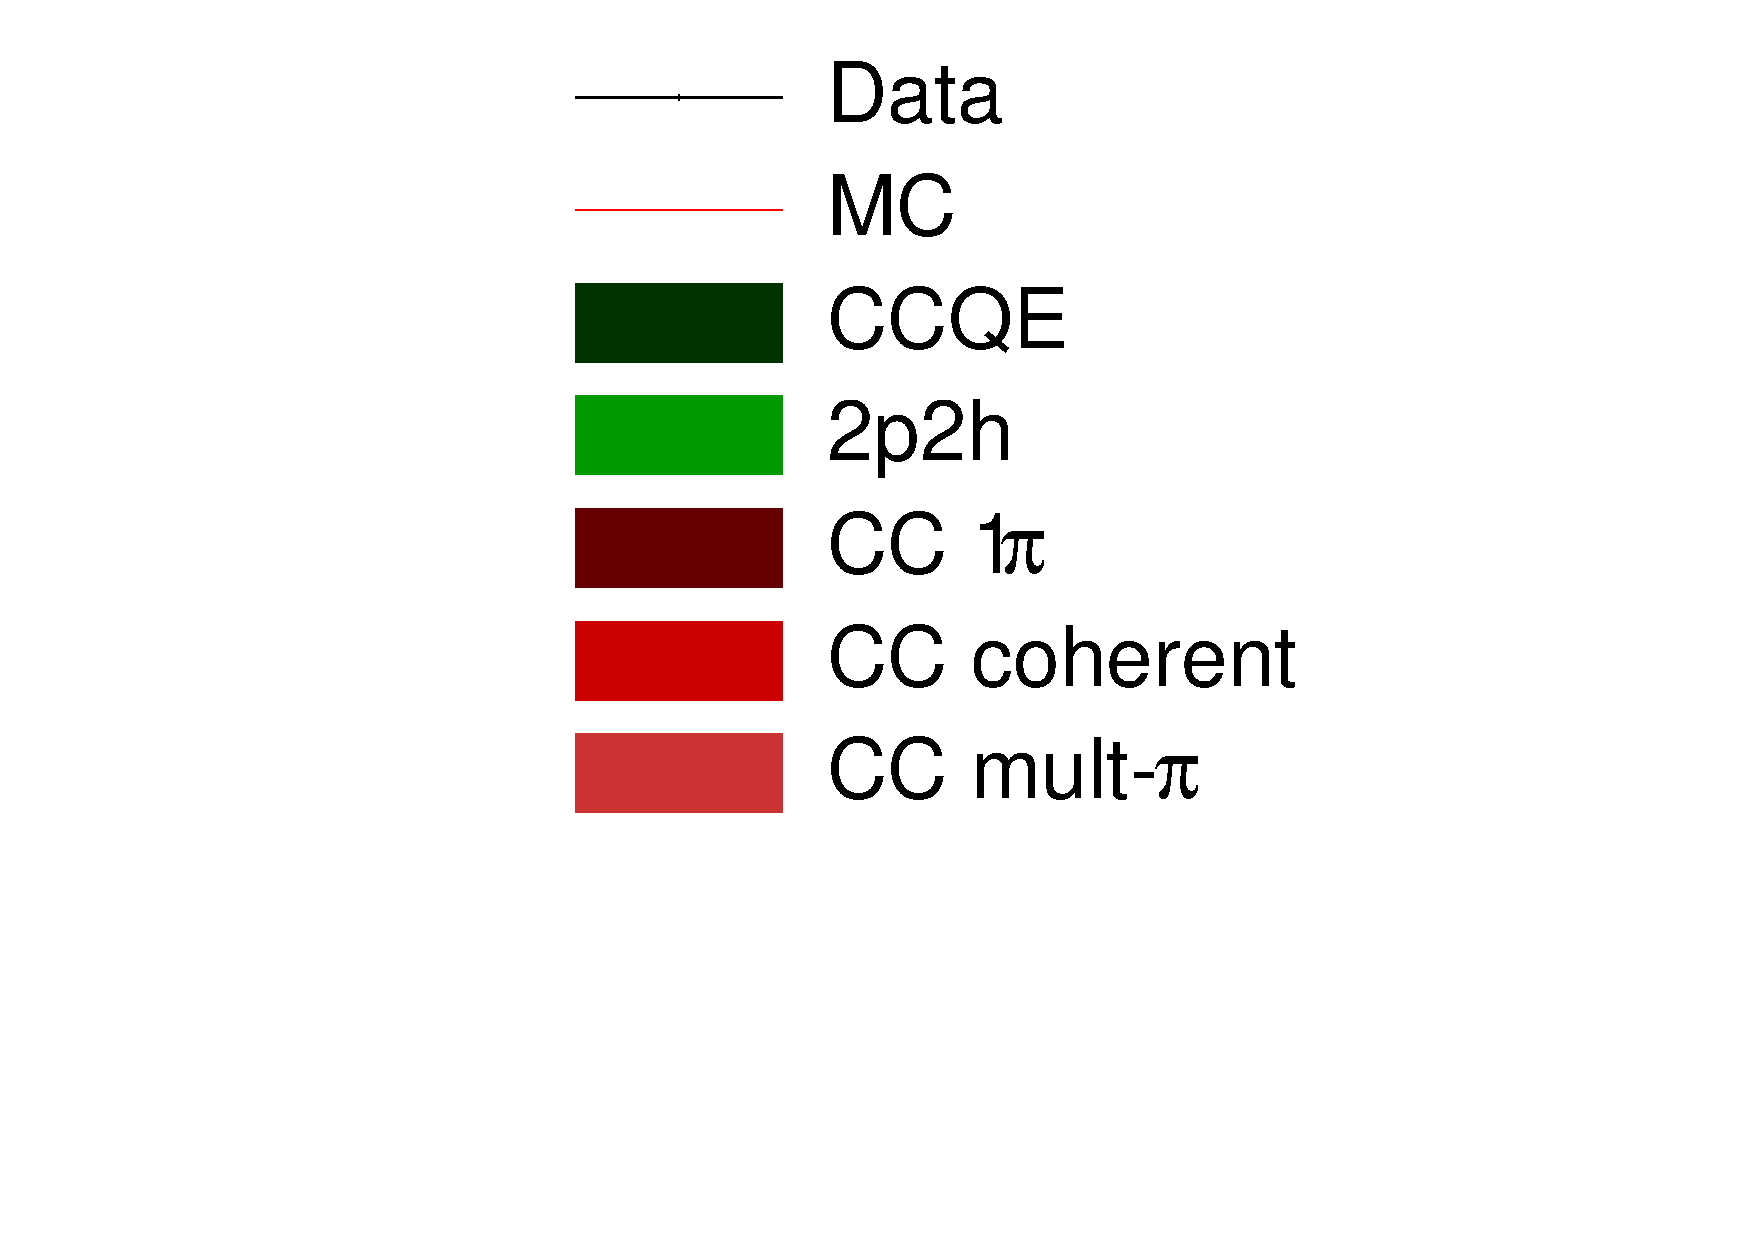
\includegraphics[width=\linewidth, trim={5mm 60mm 30mm 0mm}, clip]{figs/legend}
\end{subfigure}
\begin{subfigure}{.24\textwidth}
  \centering
  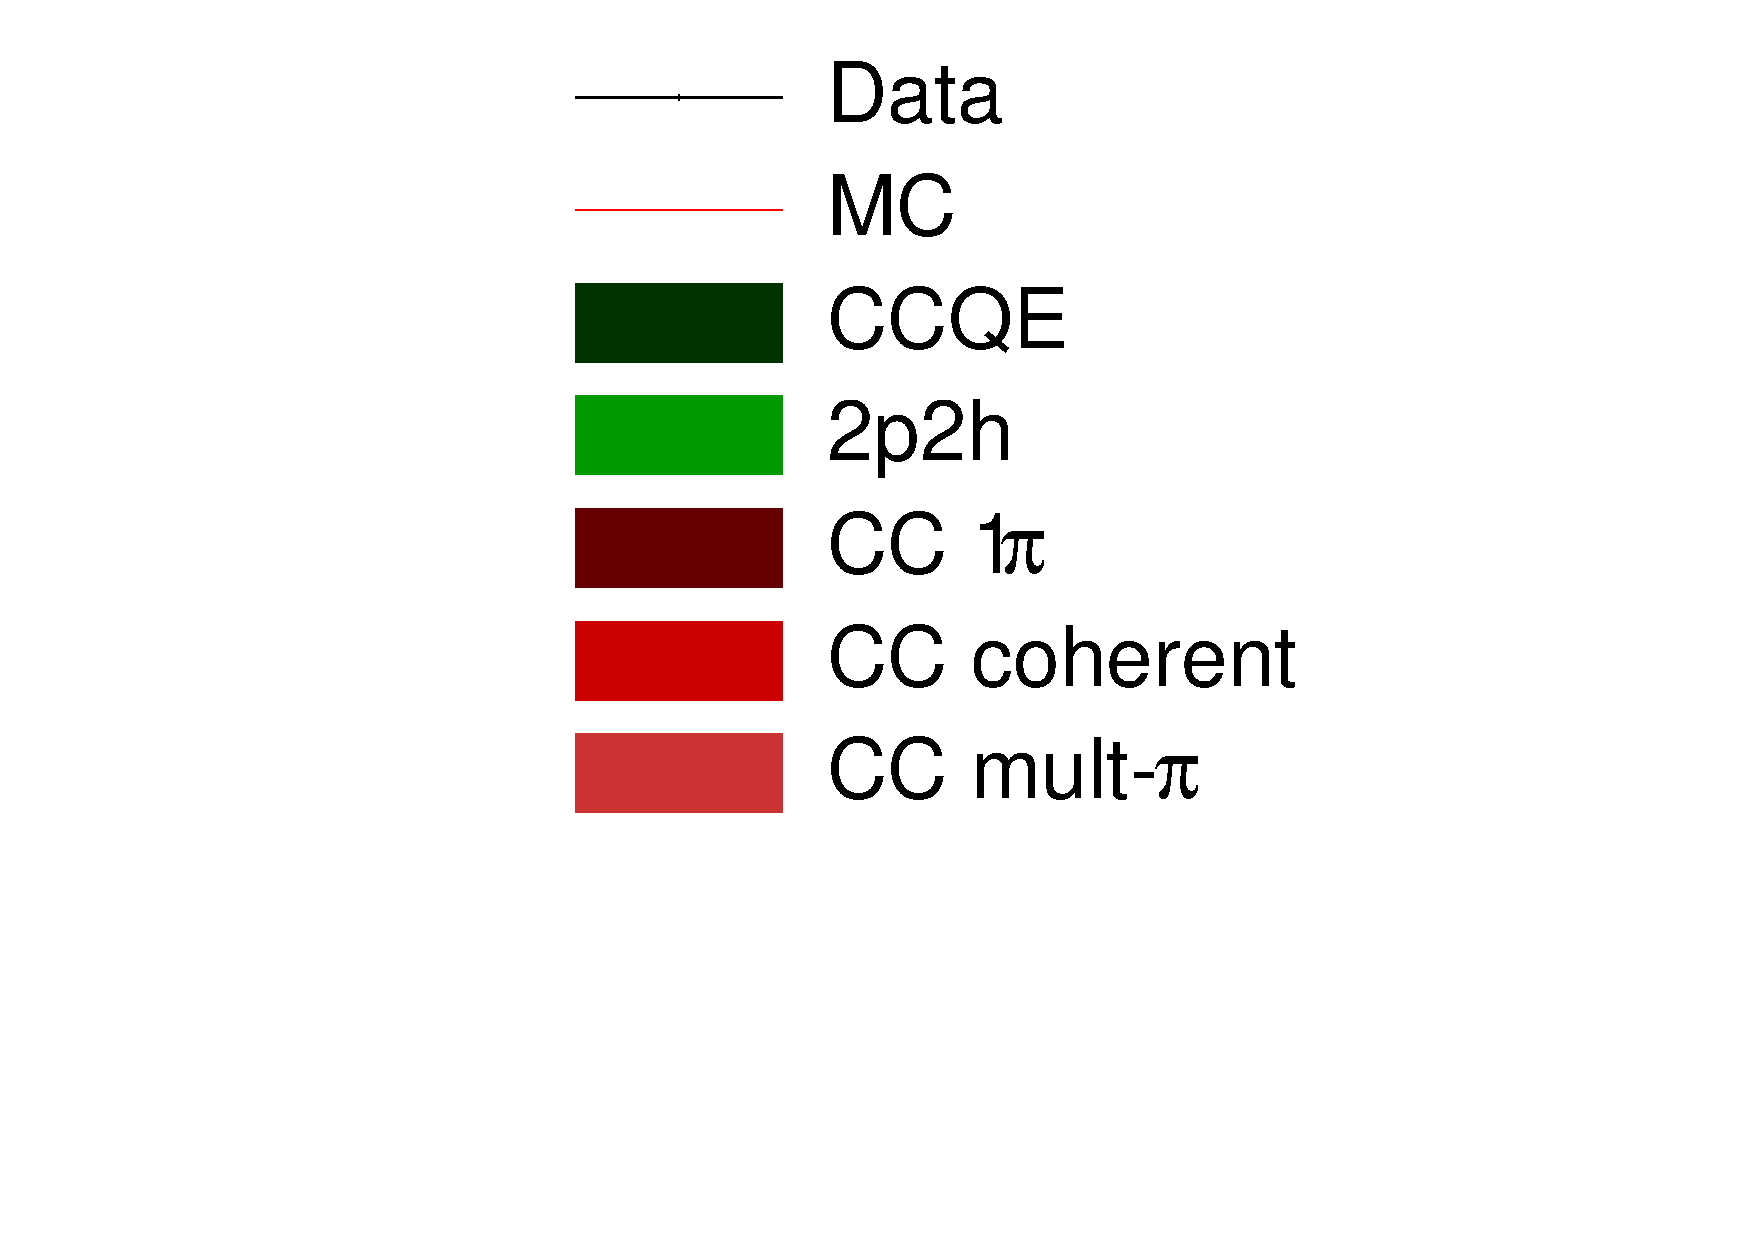
\includegraphics[width=\linewidth, trim={5mm 0mm 30mm 80mm}, clip]{figs/legend}
\end{subfigure}
\begin{subfigure}{.24\textwidth}
  \centering
  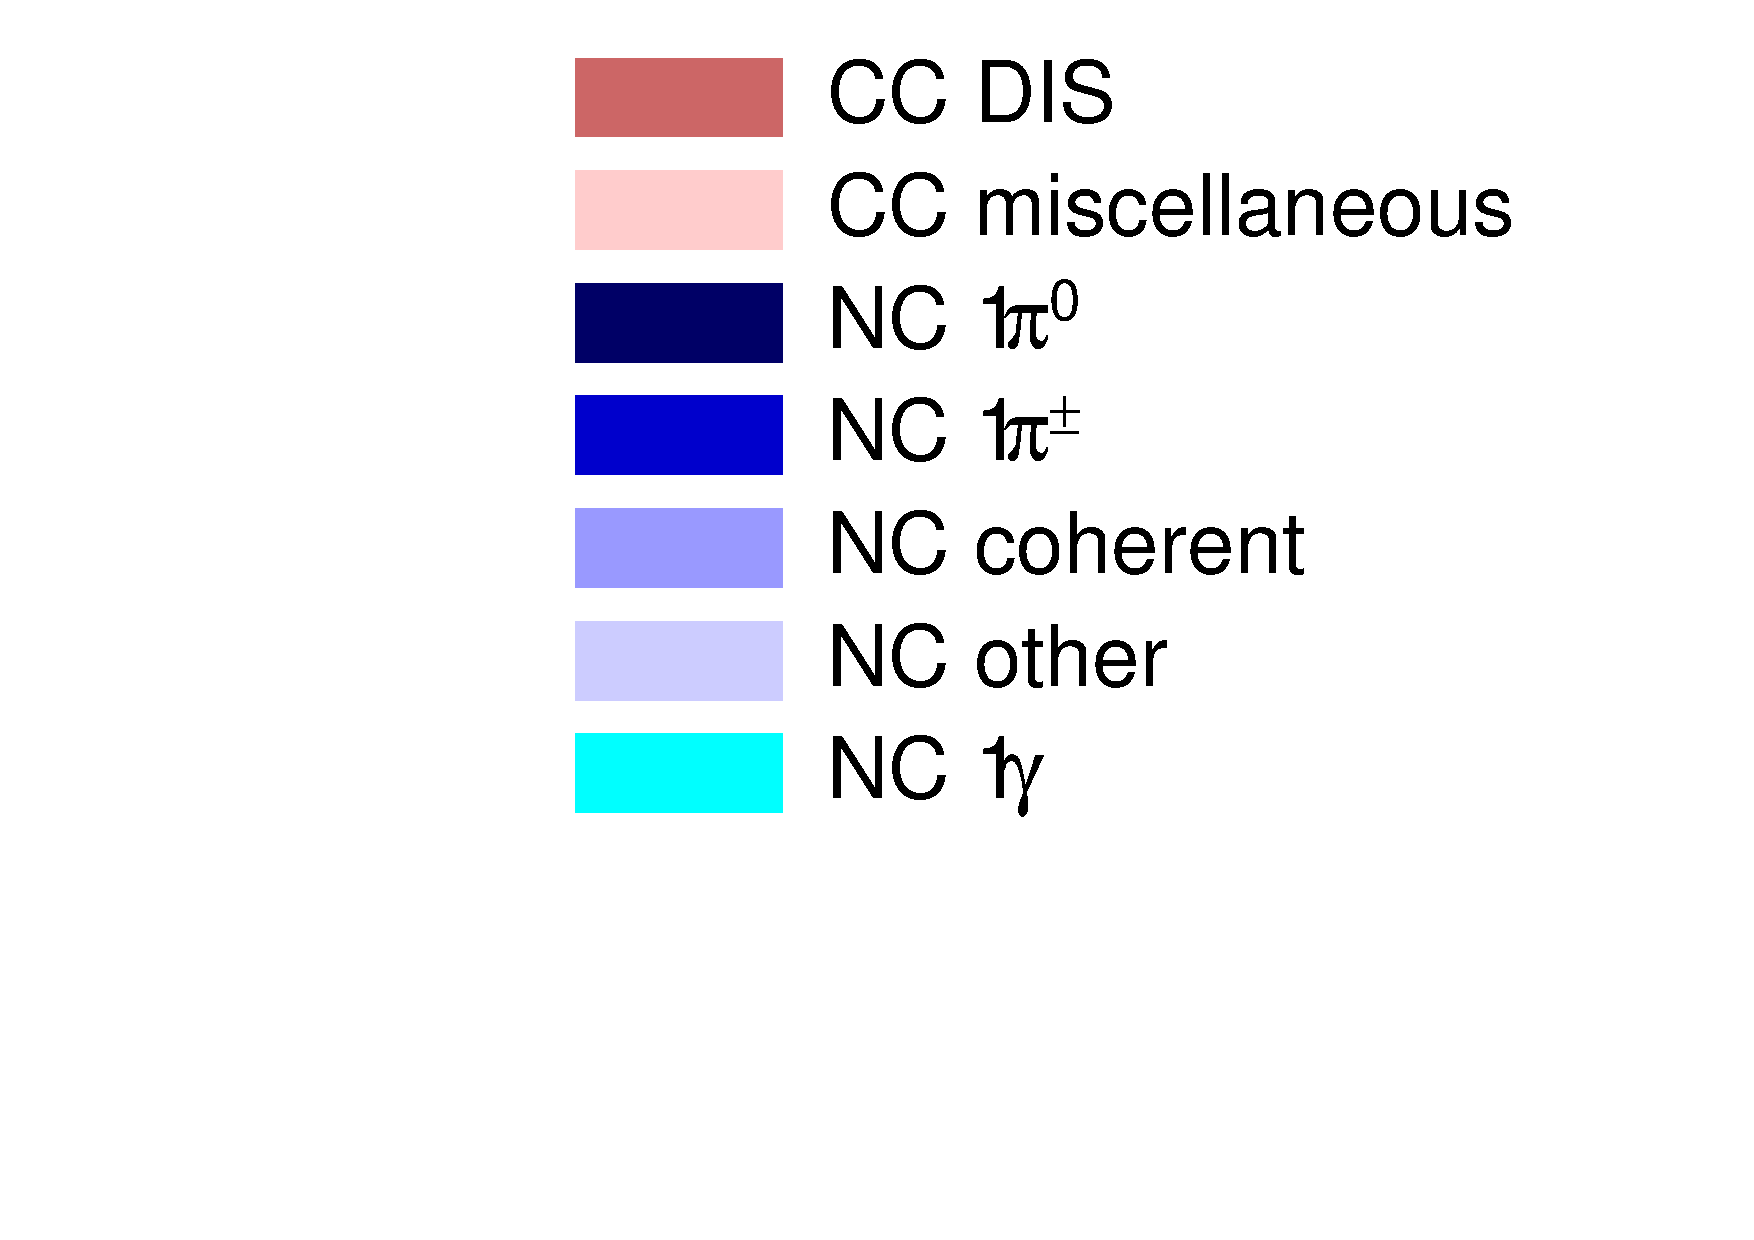
\includegraphics[width=\linewidth, trim={5mm 60mm 30mm 0mm}, clip]{figs/legend2}
\end{subfigure}
\begin{subfigure}{.24\textwidth}
  \centering
  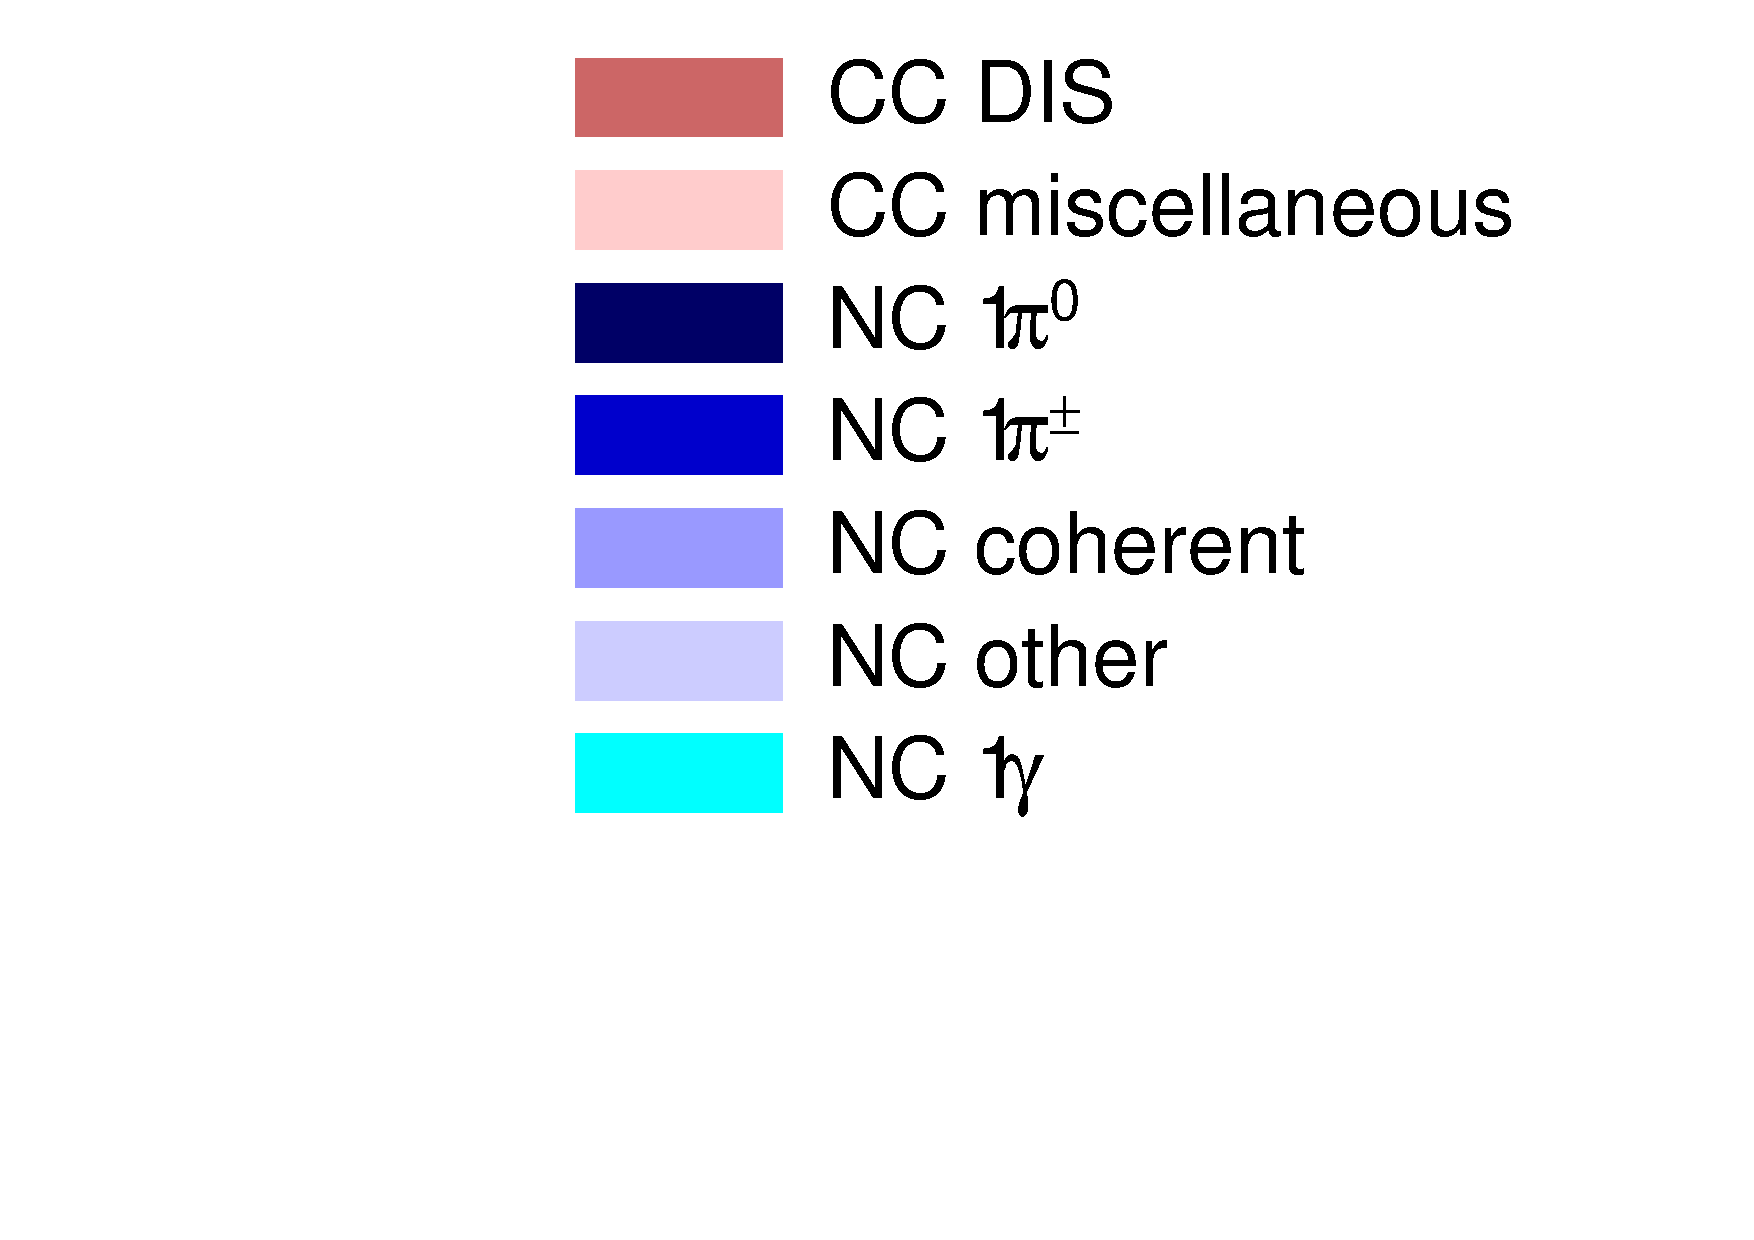
\includegraphics[width=\linewidth, trim={5mm 0mm 30mm 80mm}, clip]{figs/legend2}
\end{subfigure}

\begin{subfigure}{0.49\textwidth}
  \centering
  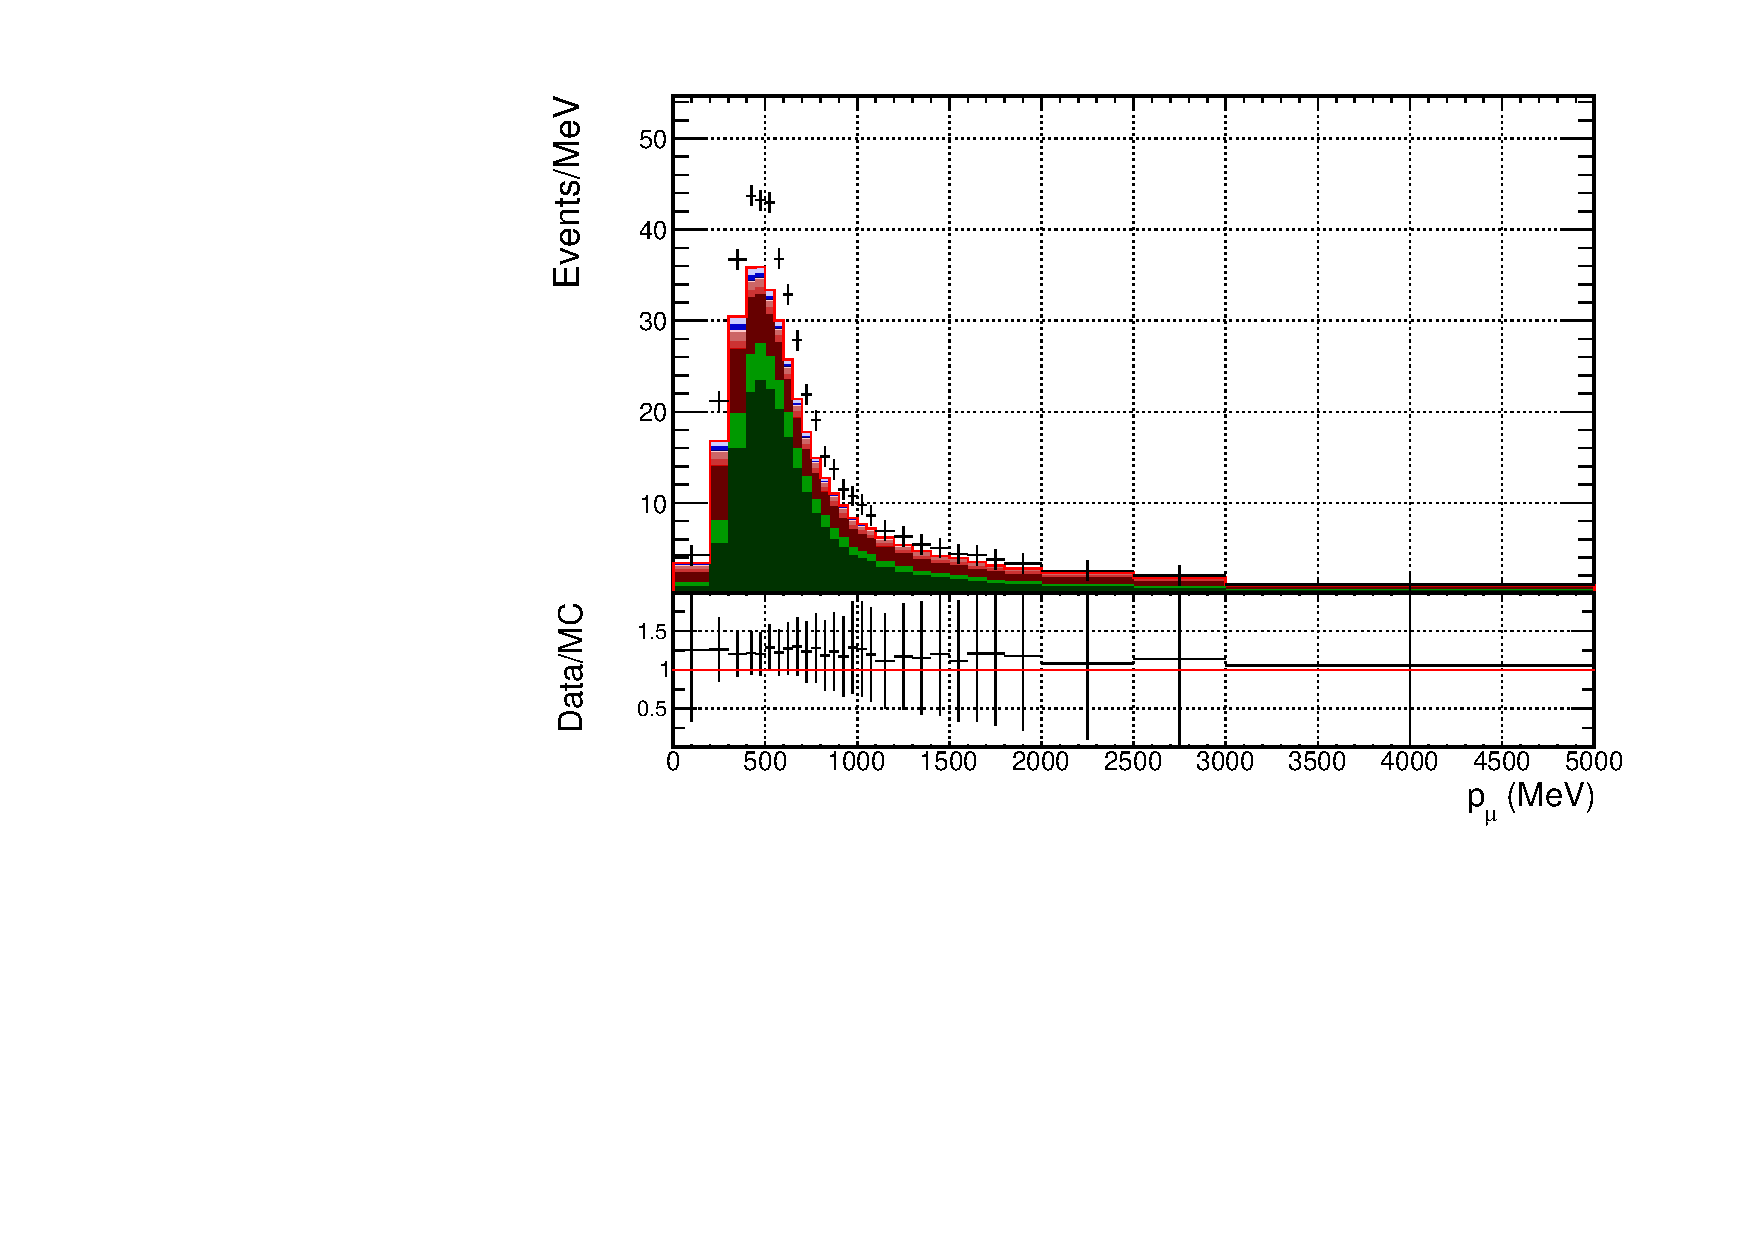
\includegraphics[width=\textwidth]{figs/FGD1_numuCC_0pi_p}
  \caption{FGD1 FHC $\nu_{\mu}$ 0$\pi$}
\end{subfigure}
\begin{subfigure}{0.49\textwidth}
  \centering
  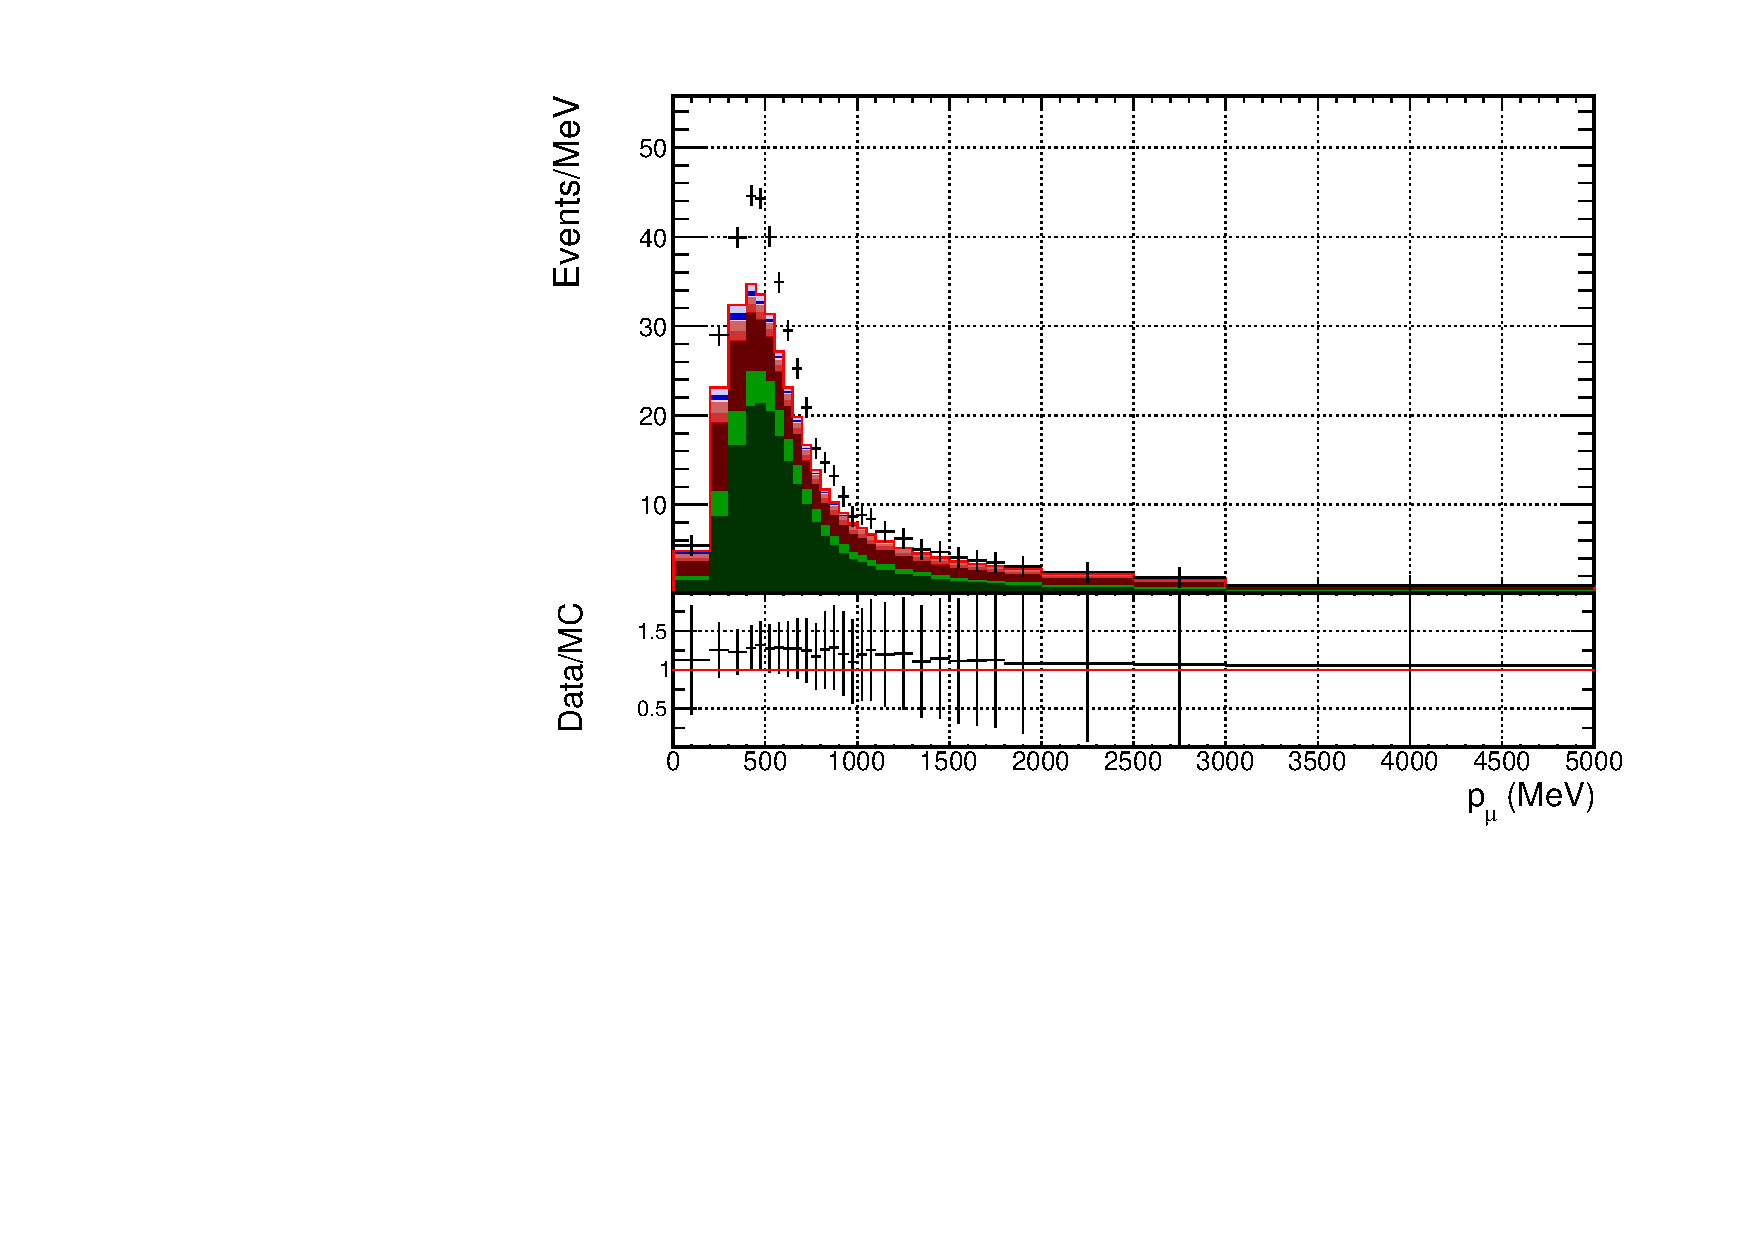
\includegraphics[width=\textwidth]{figs/FGD2_numuCC_0pi_p}
  \caption{FGD2 FHC $\nu_{\mu}$ 0$\pi$}
\end{subfigure}

\begin{subfigure}{0.49\textwidth}
  \centering
  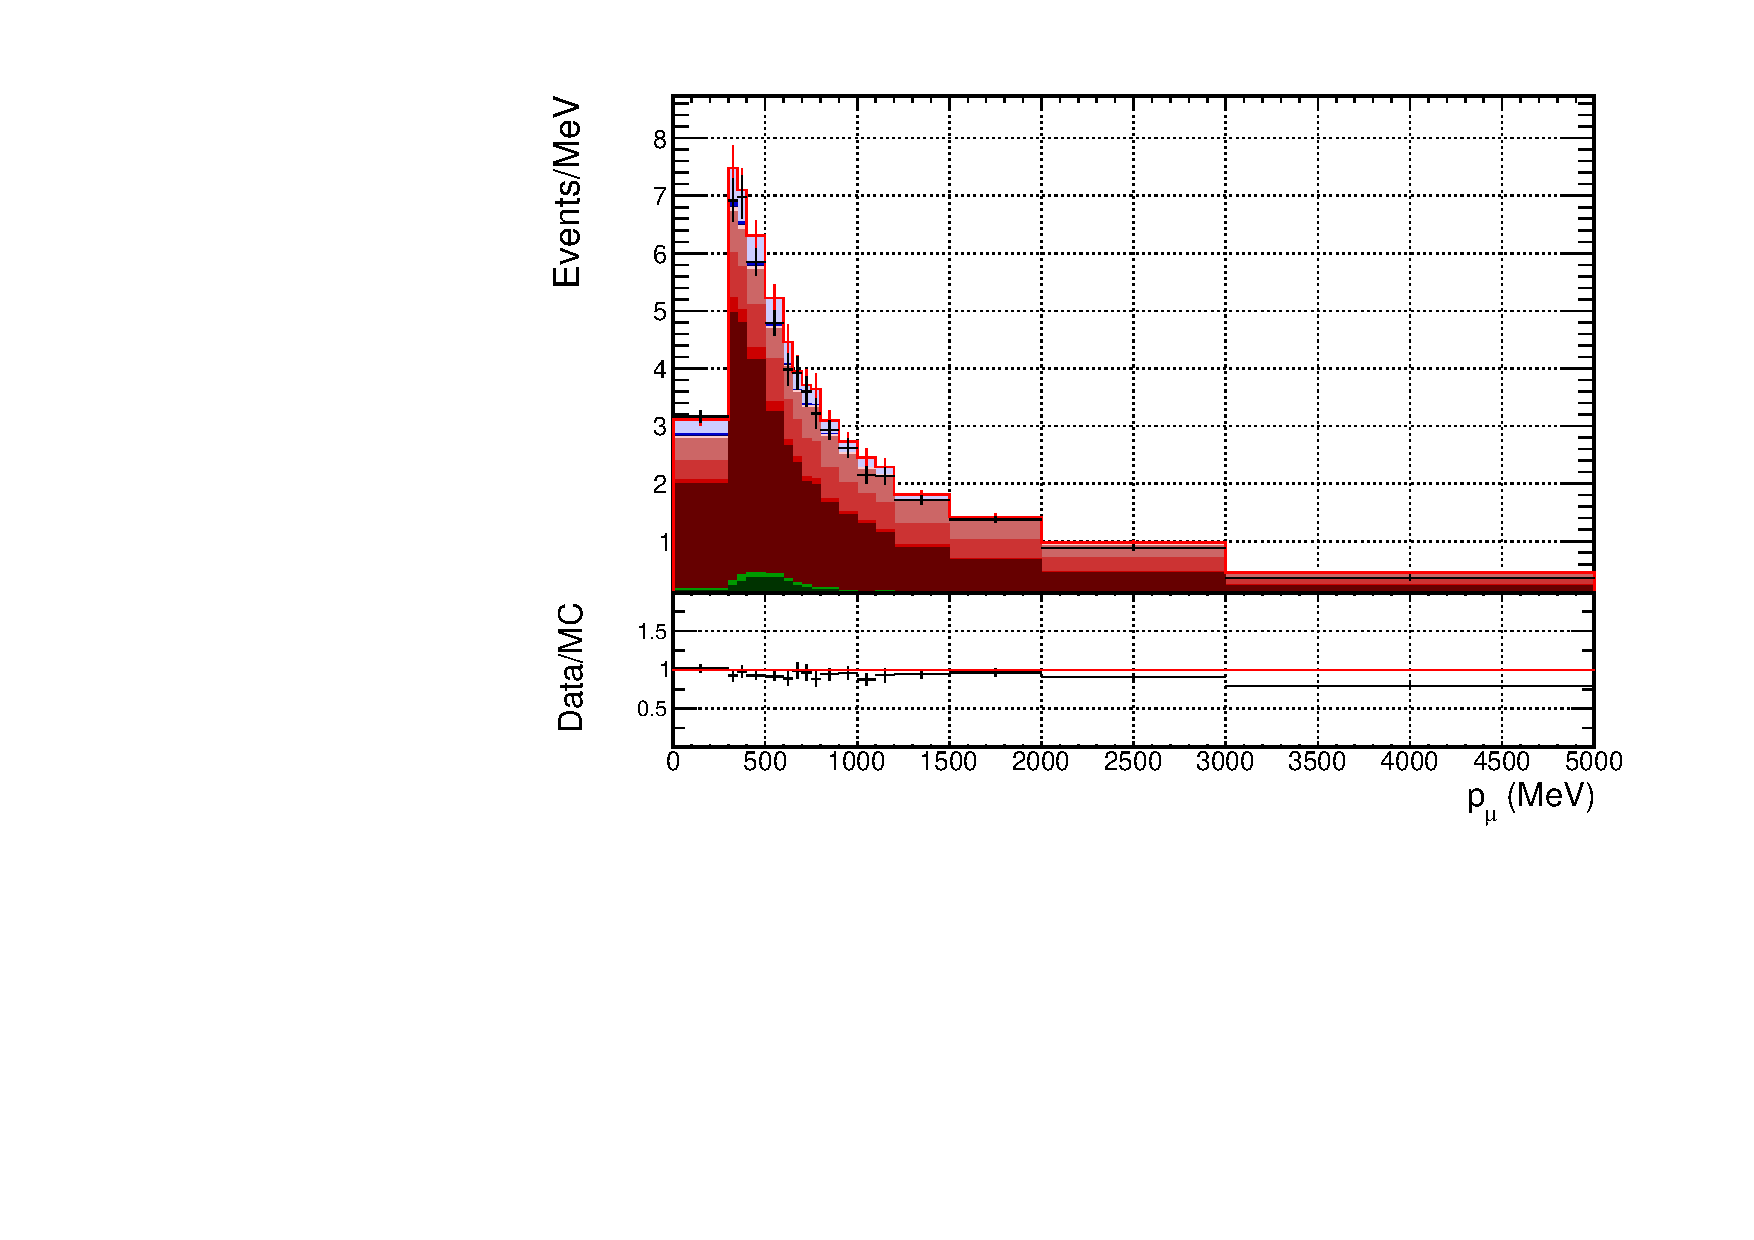
\includegraphics[width=\textwidth]{figs/FGD1_numuCC_1pi_p}
  \caption{FGD1 FHC $\nu_{\mu}$ 1$\pi$}
\end{subfigure}
\begin{subfigure}{0.49\textwidth}
  \centering
  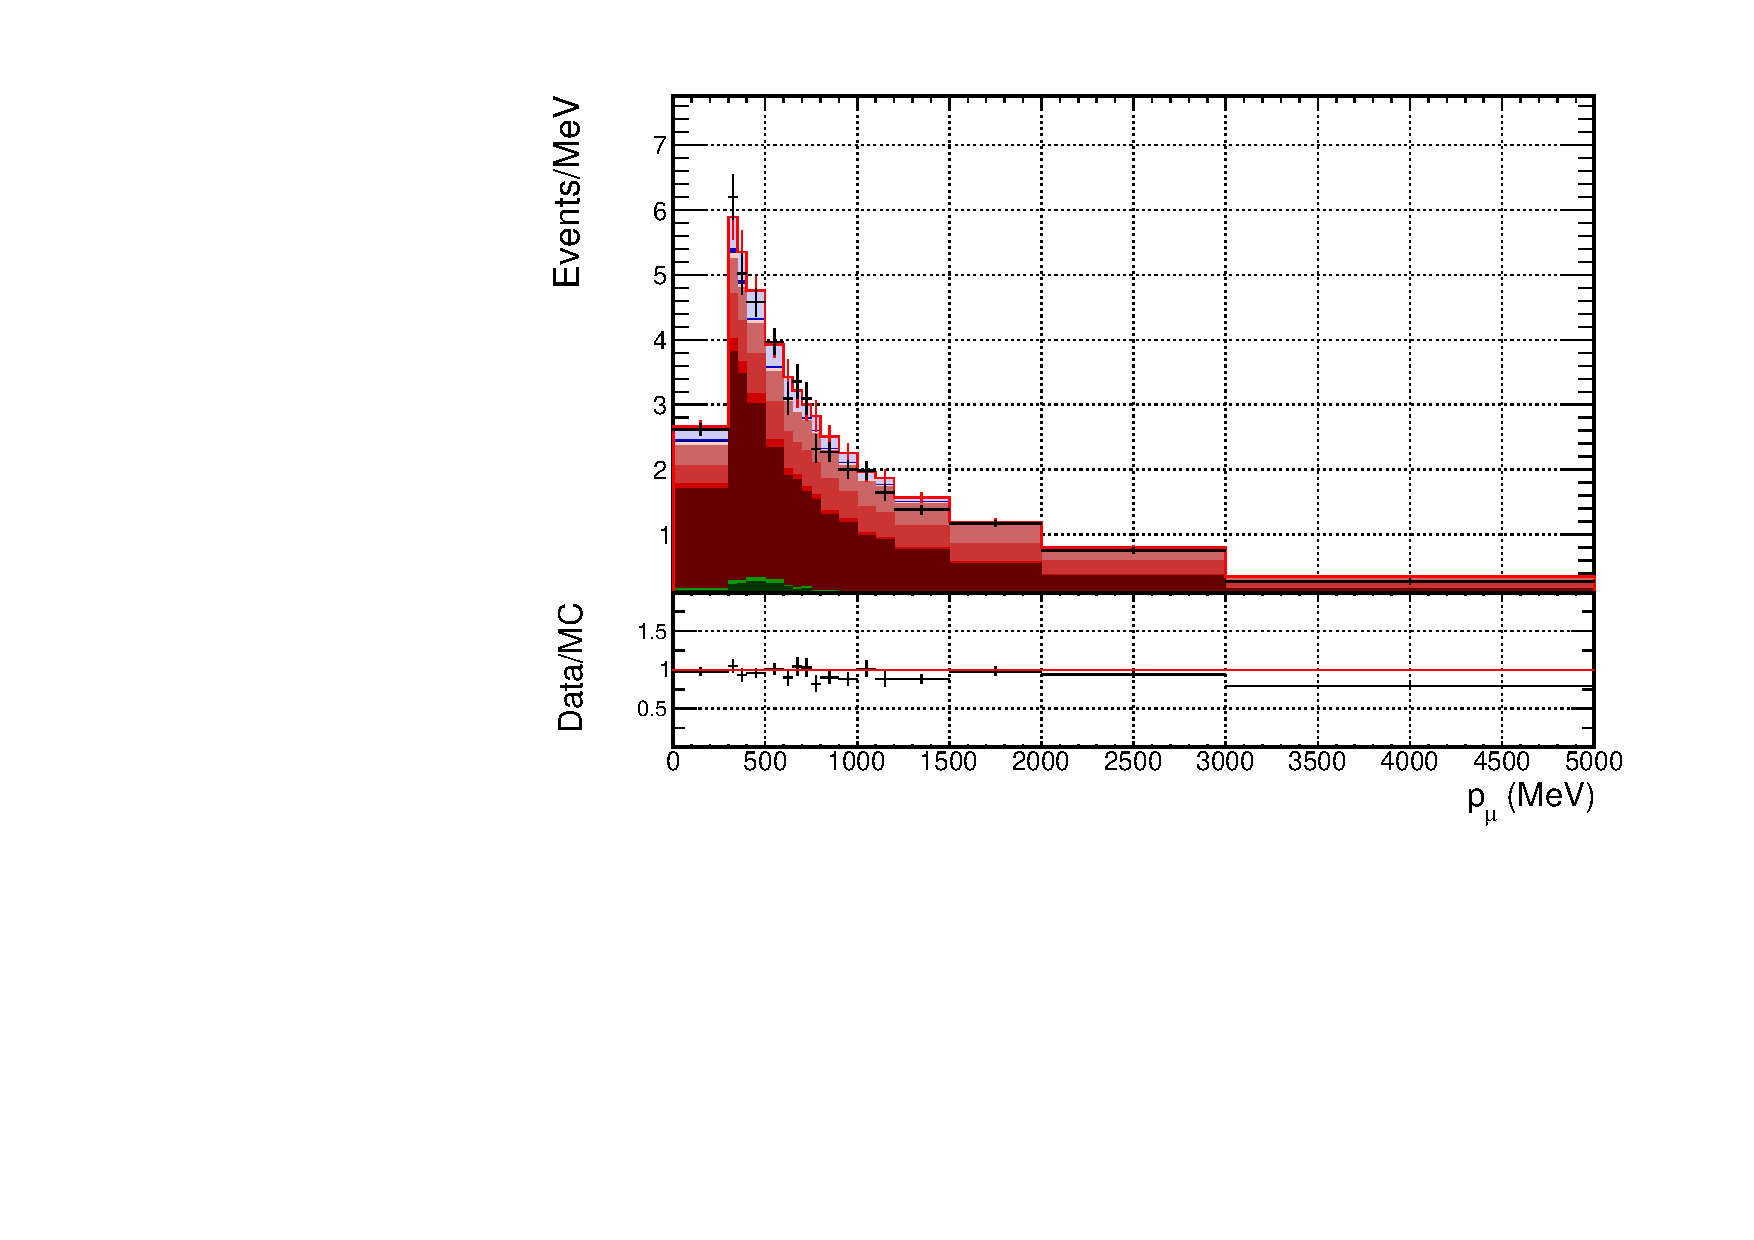
\includegraphics[width=\textwidth]{figs/FGD2_numuCC_1pi_p}
  \caption{FGD2 FHC $\nu_{\mu}$ 1$\pi$}
\end{subfigure}

\begin{subfigure}{0.49\textwidth}
  \centering
  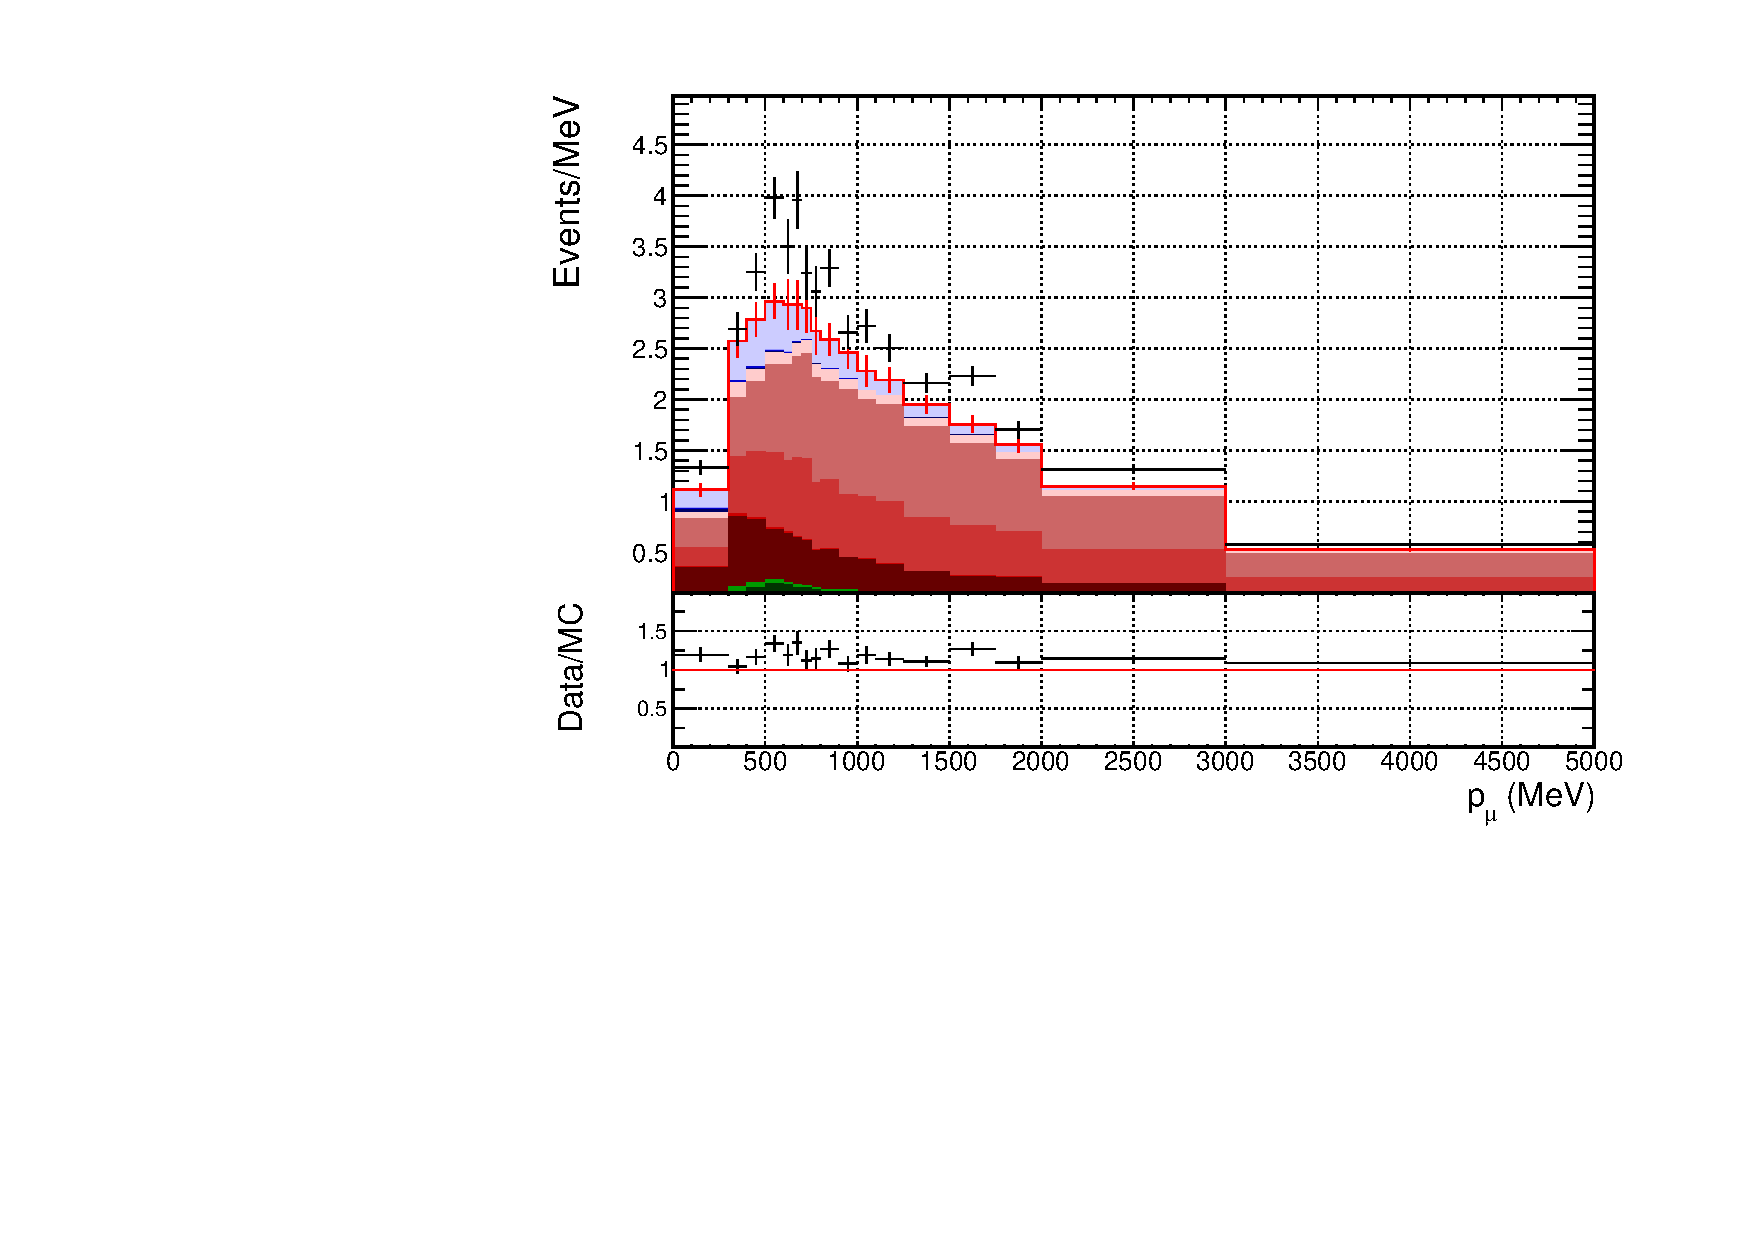
\includegraphics[width=\textwidth]{figs/FGD1_numuCC_other_p}
  \caption{FGD1 FHC $\nu_{\mu}$ Other}
\end{subfigure}
\begin{subfigure}{0.49\textwidth}
  \centering
  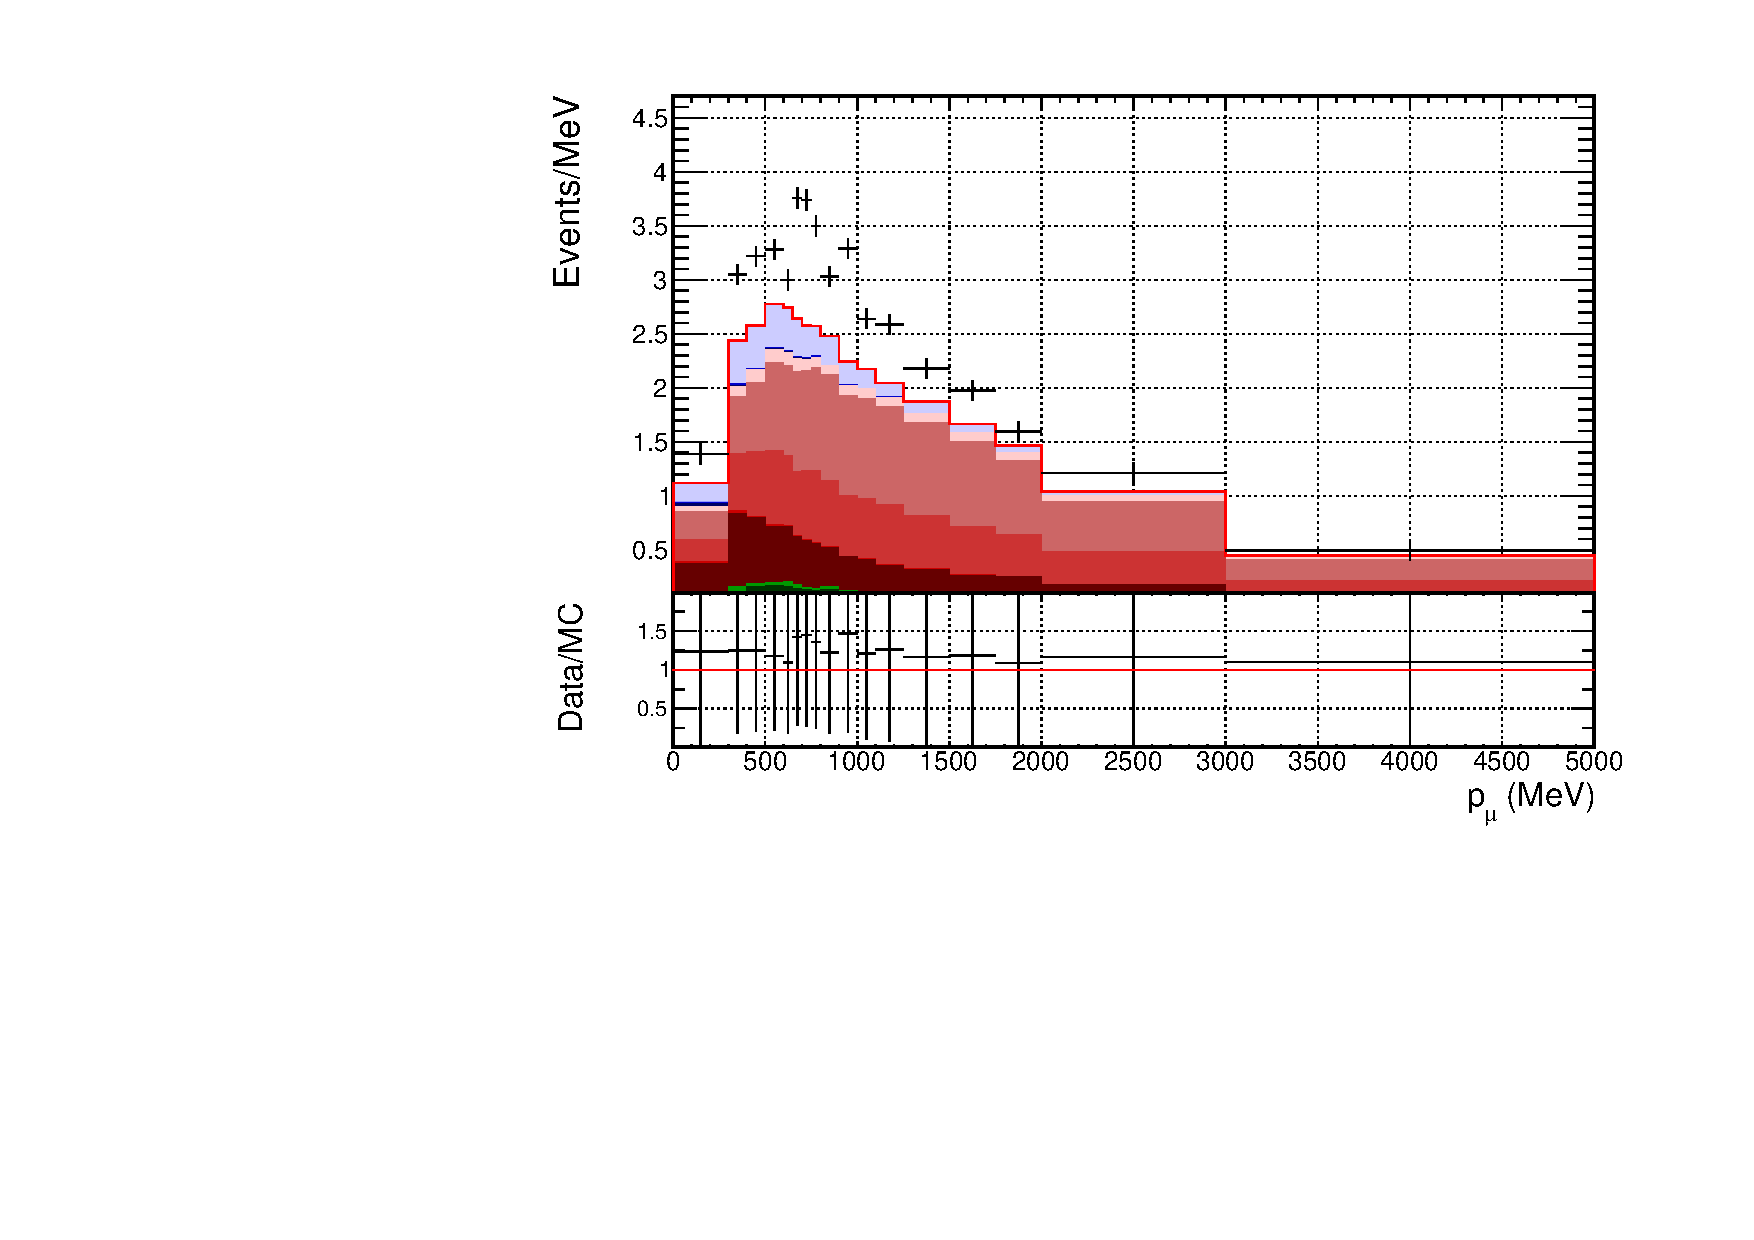
\includegraphics[width=\textwidth]{figs/FGD2_numuCC_other_p}
  \caption{FGD2 FHC $\nu_{\mu}$ Other}
\end{subfigure}
\caption{$p_{\mu}$ projections of data and nominal MC broken down by interaction mode for FHC selections.}
\label{fig:pstack_fhcapp}
\end{figure}

\begin{figure}[!htbp]
\centering
\begin{subfigure}{.24\textwidth}
  \centering
  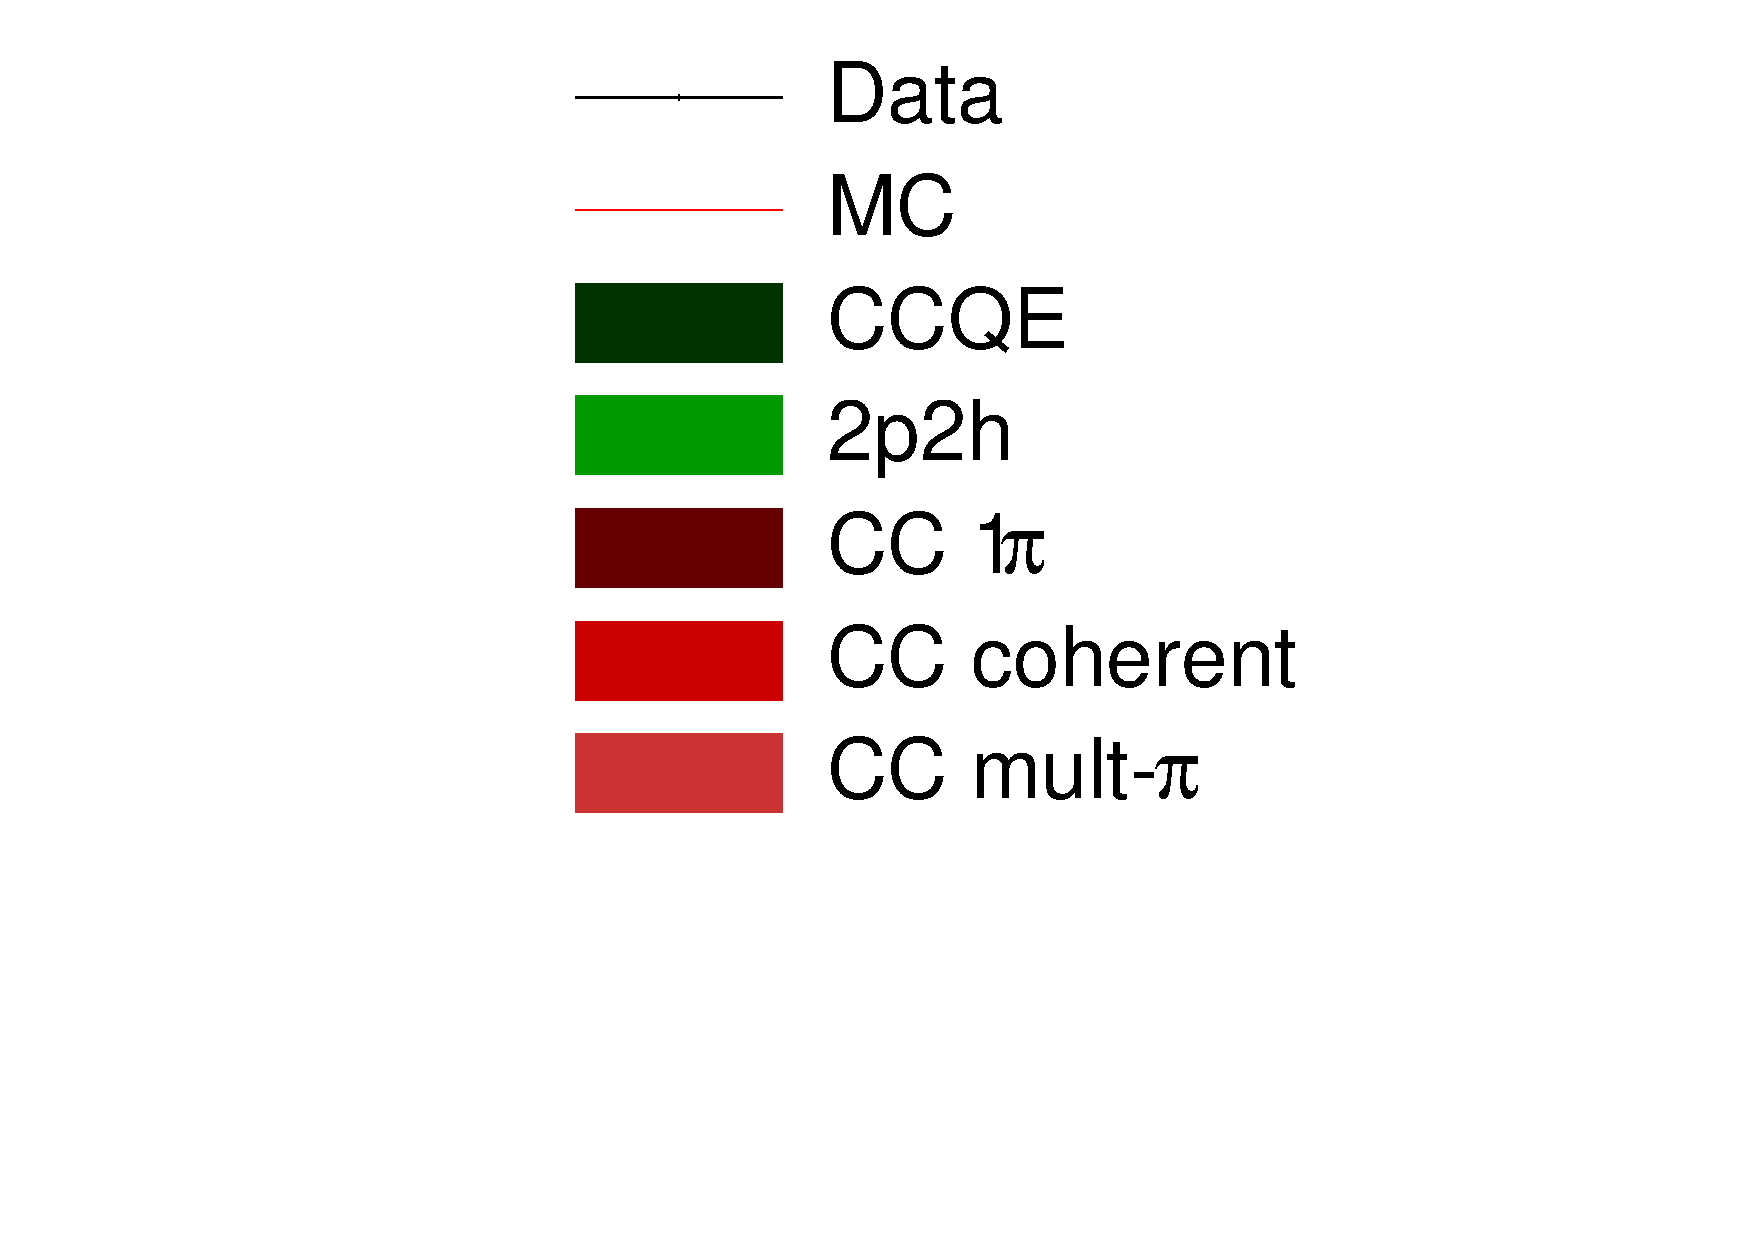
\includegraphics[width=\linewidth, trim={5mm 60mm 30mm 0mm}, clip]{figs/legend}
\end{subfigure}
\begin{subfigure}{.24\textwidth}
  \centering
  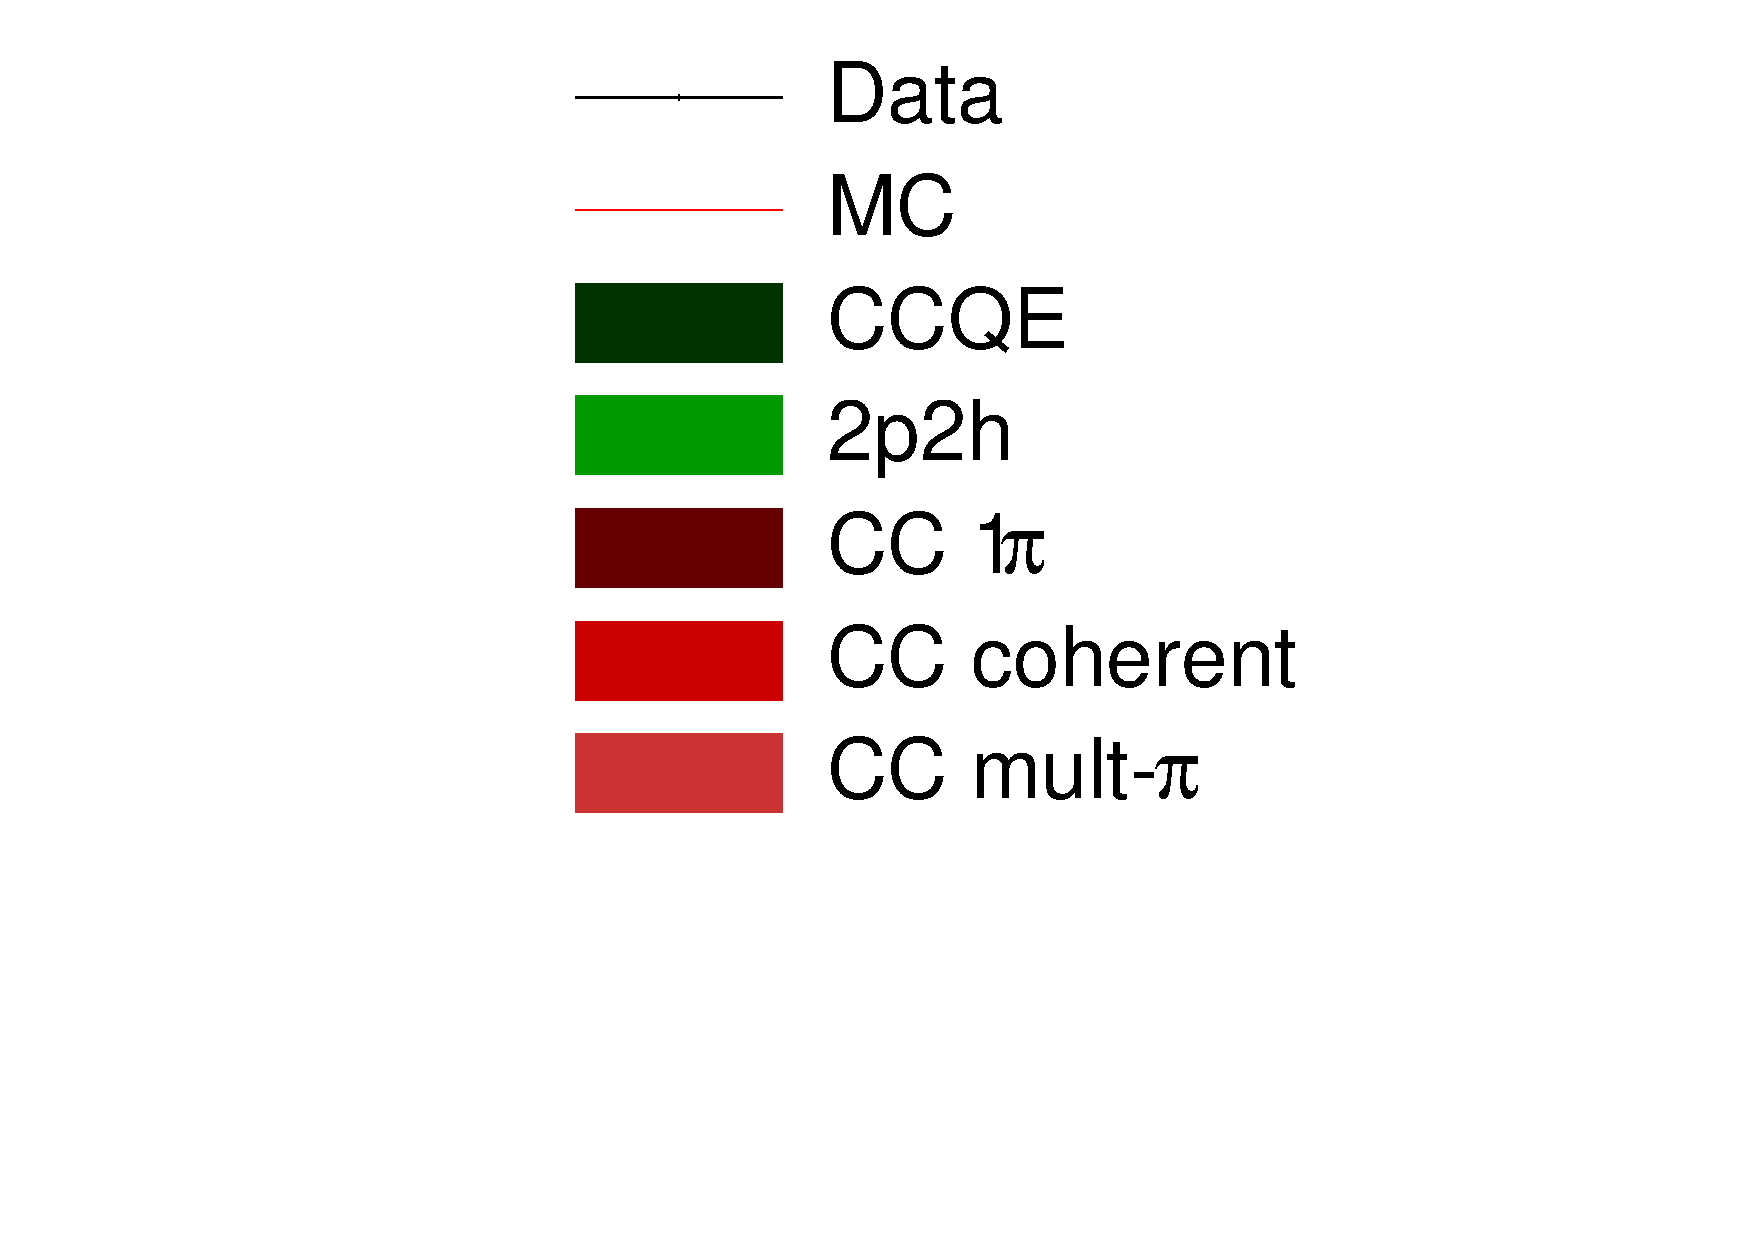
\includegraphics[width=\linewidth, trim={5mm 0mm 30mm 80mm}, clip]{figs/legend}
\end{subfigure}
\begin{subfigure}{.24\textwidth}
  \centering
  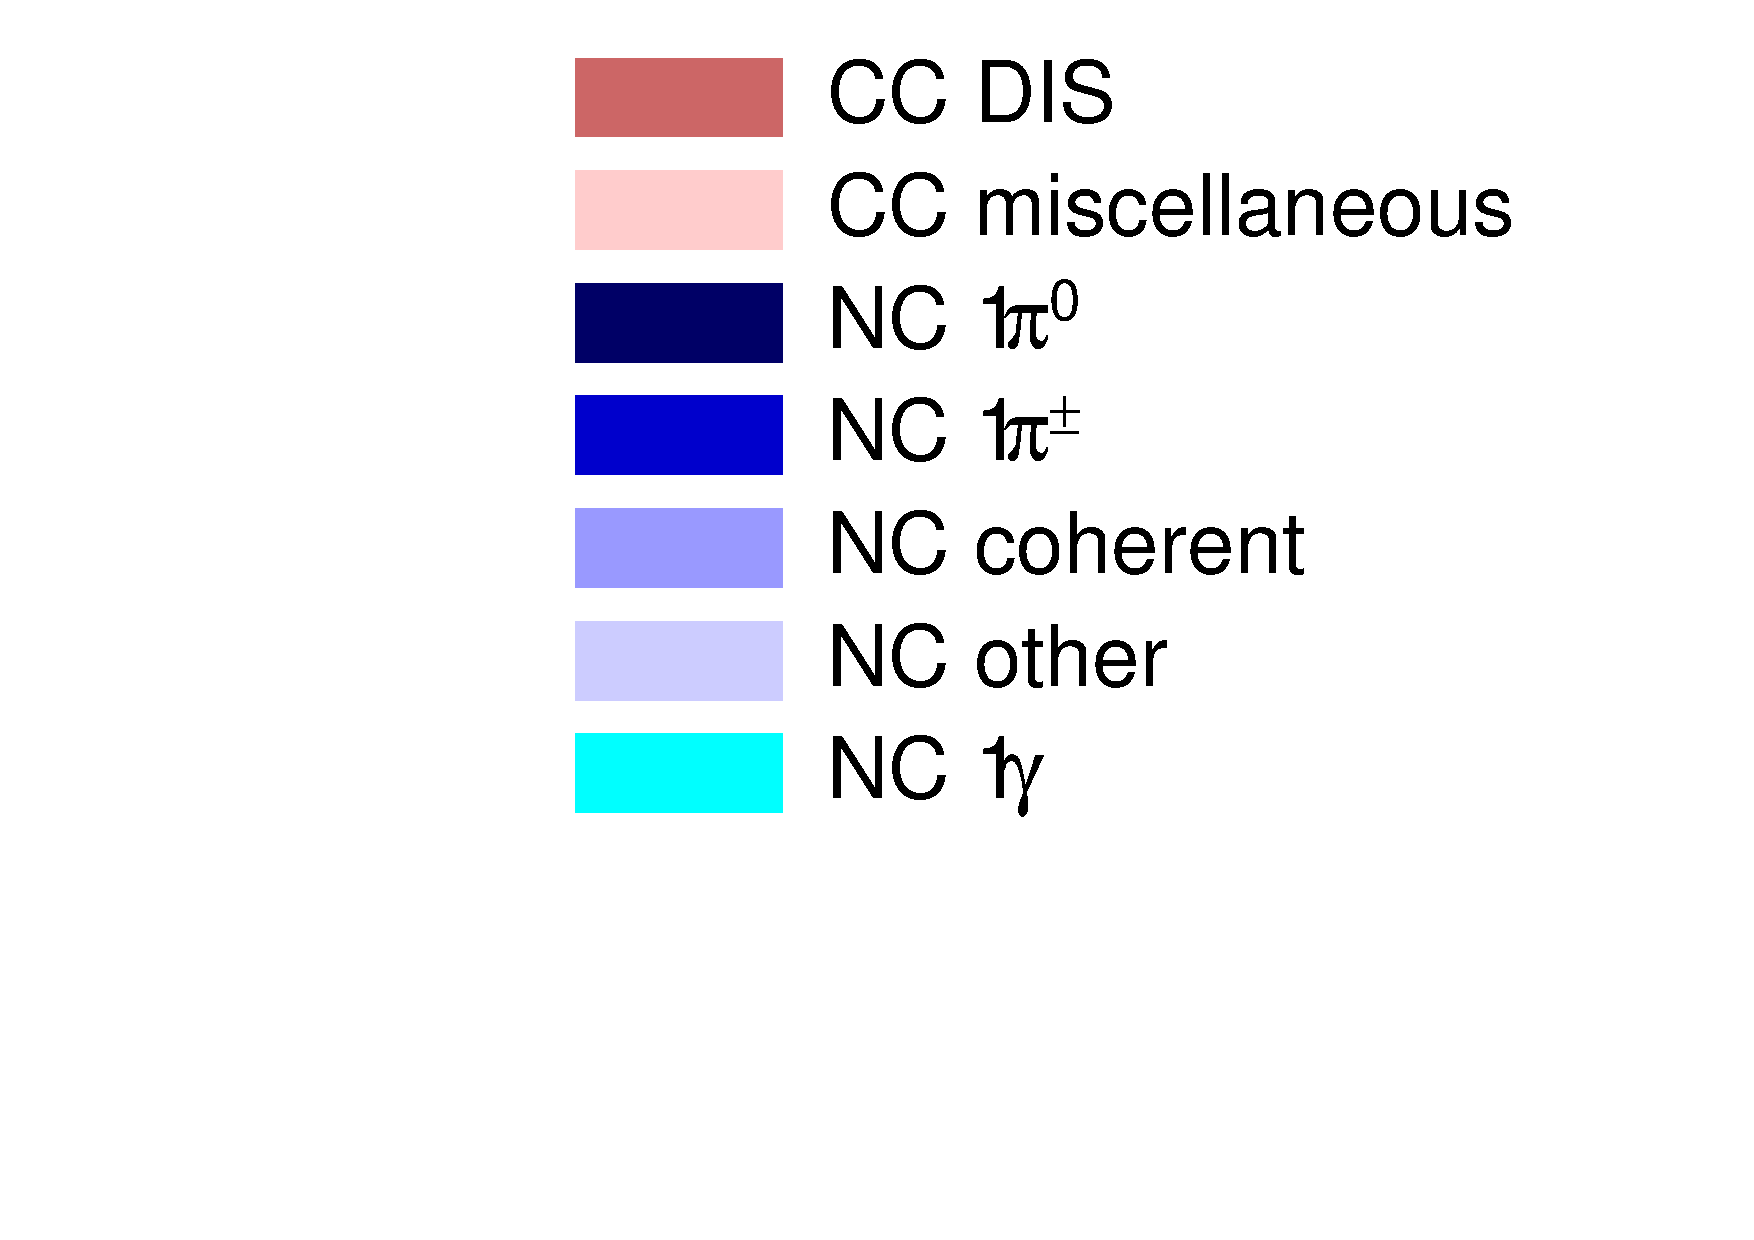
\includegraphics[width=\linewidth, trim={5mm 60mm 30mm 0mm}, clip]{figs/legend2}
\end{subfigure}
\begin{subfigure}{.24\textwidth}
  \centering
  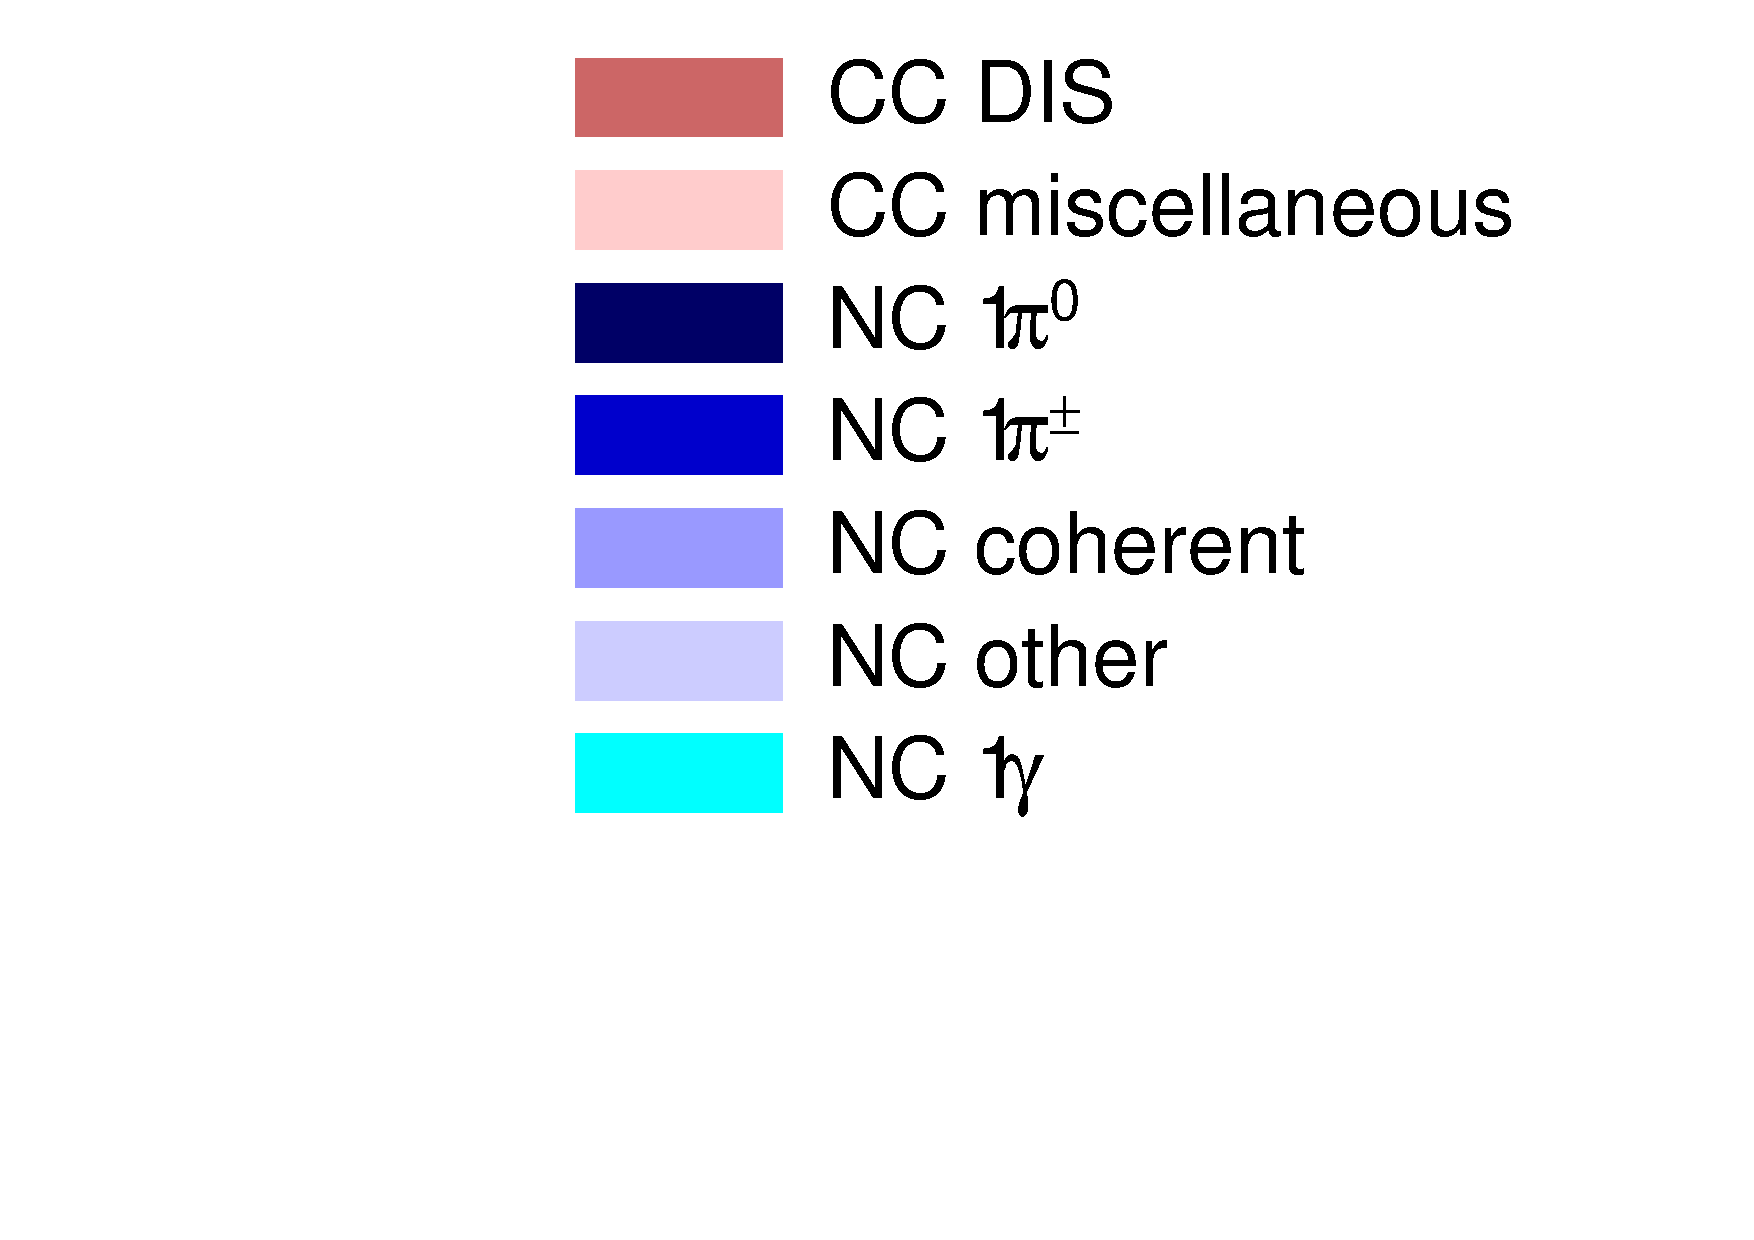
\includegraphics[width=\linewidth, trim={5mm 0mm 30mm 80mm}, clip]{figs/legend2}
\end{subfigure}

\begin{subfigure}{0.49\textwidth}
  \centering
  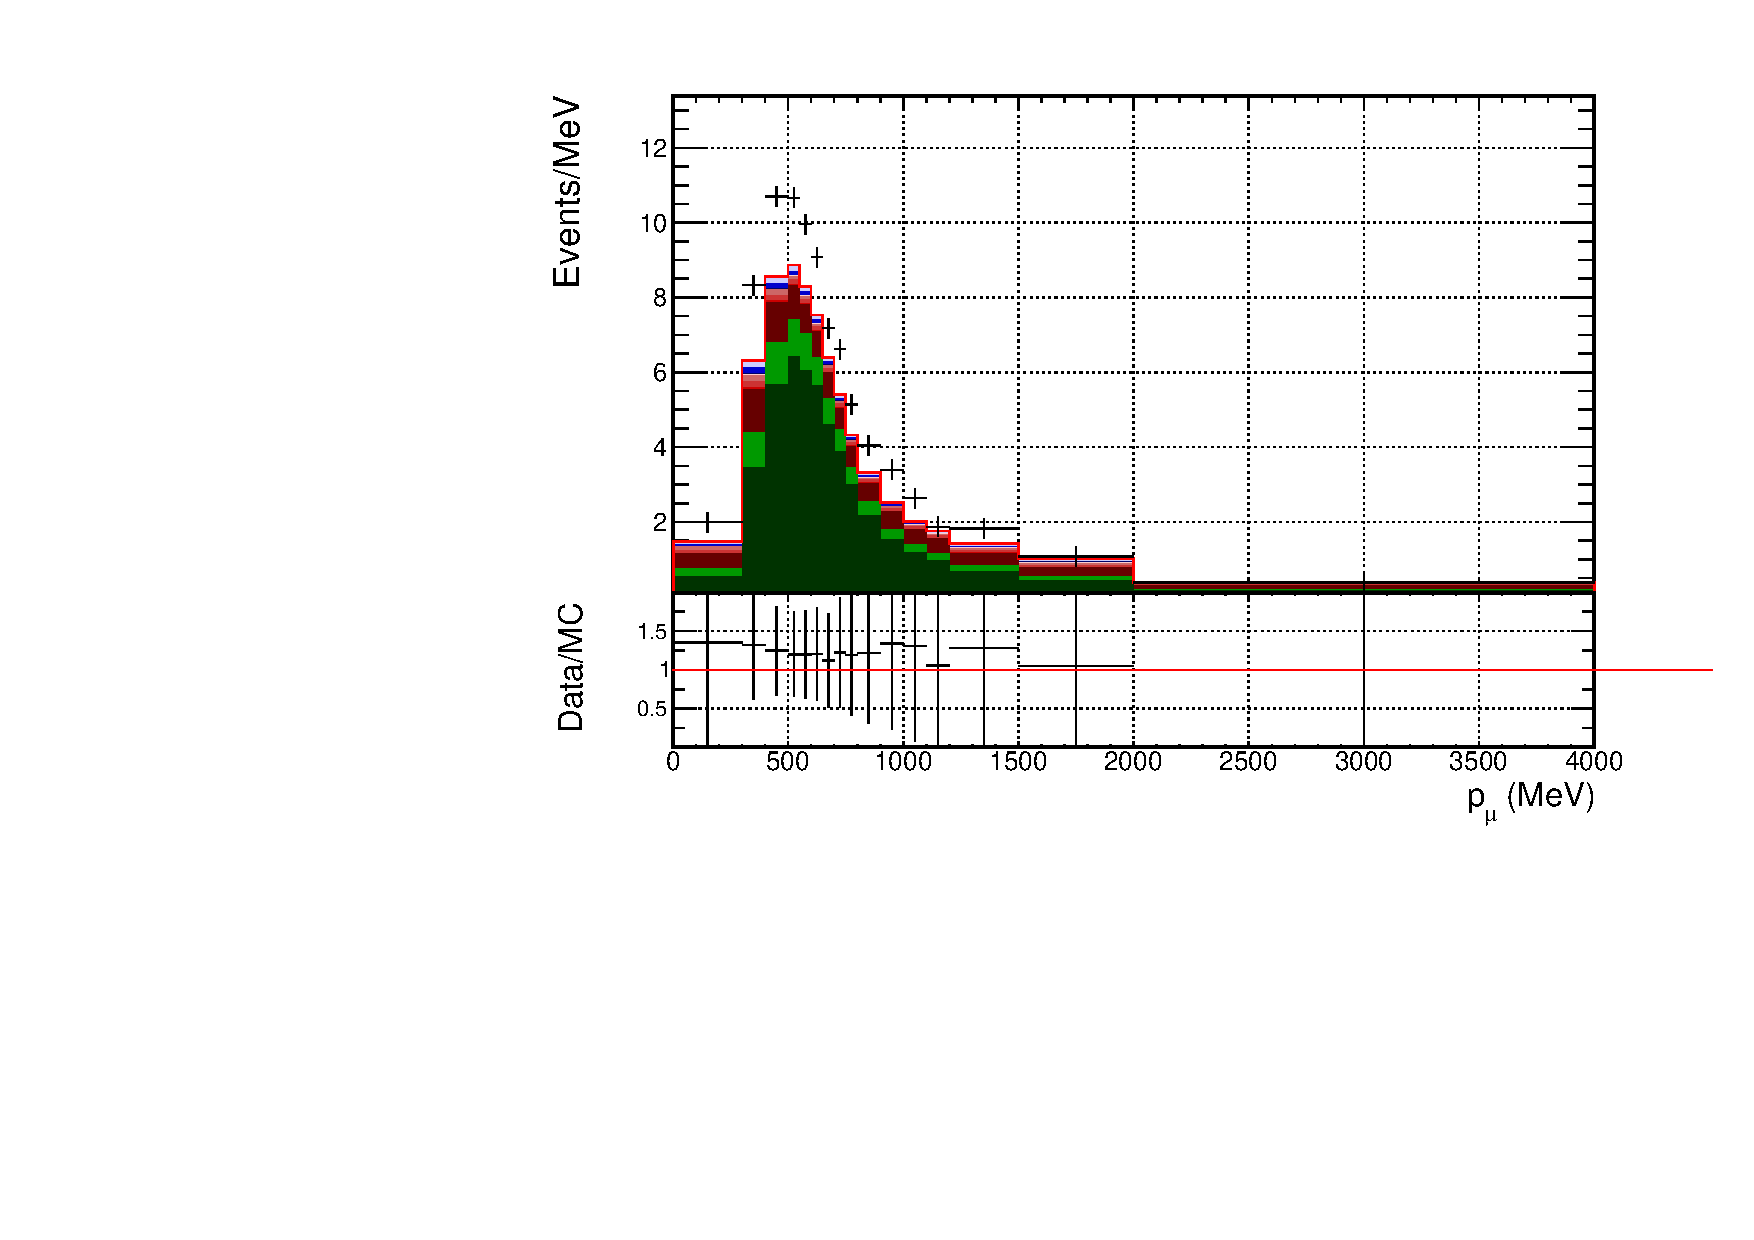
\includegraphics[width=\textwidth]{figs/FGD1_anti-numuCC_0pi_p}
  \caption{FGD1 RHC $\bar{\nu_{\mu}}$ 0$\pi$}
\end{subfigure}
\begin{subfigure}{0.49\textwidth}
  \centering
  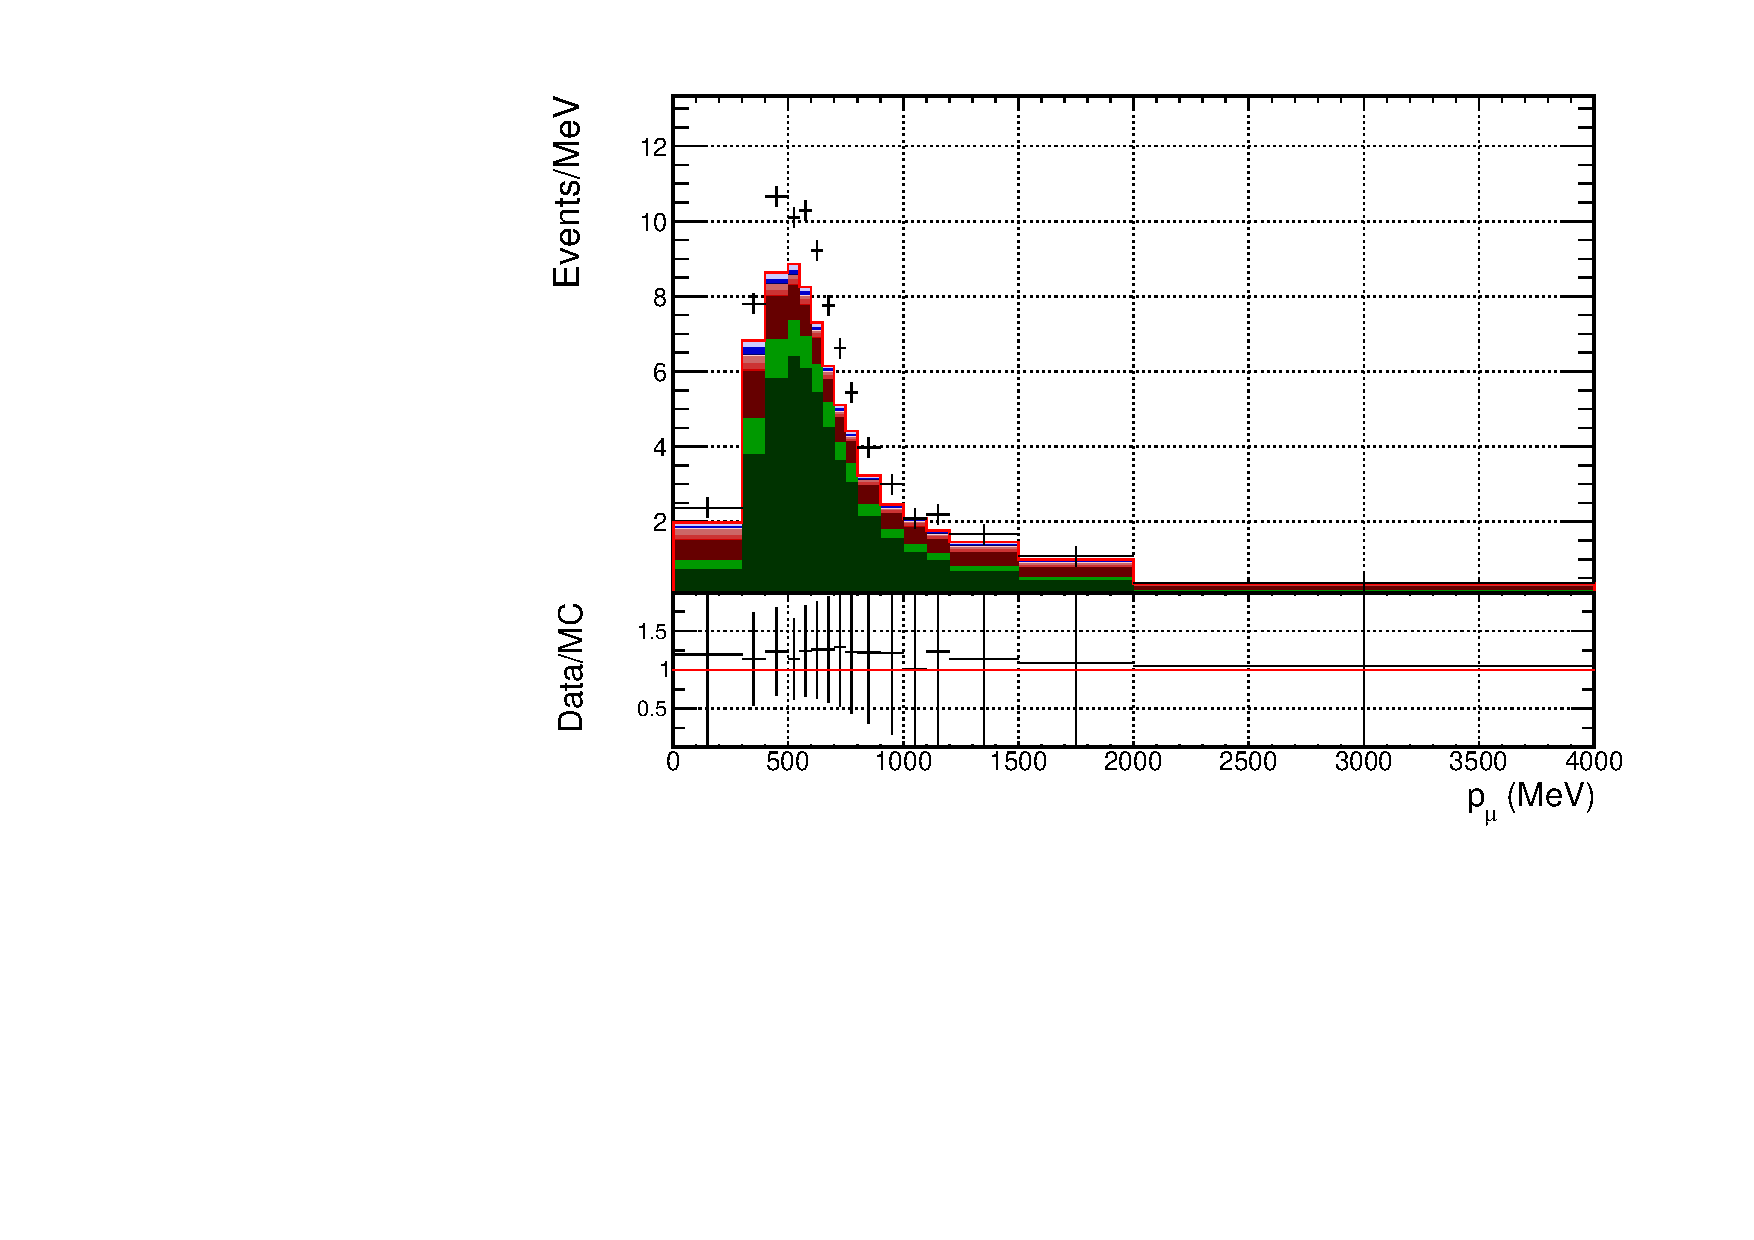
\includegraphics[width=\textwidth]{figs/FGD2_anti-numuCC_0pi_p}
  \caption{FGD2 RHC $\bar{\nu_{\mu}}$ 0$\pi$}
\end{subfigure}

\begin{subfigure}{0.49\textwidth}
  \centering
  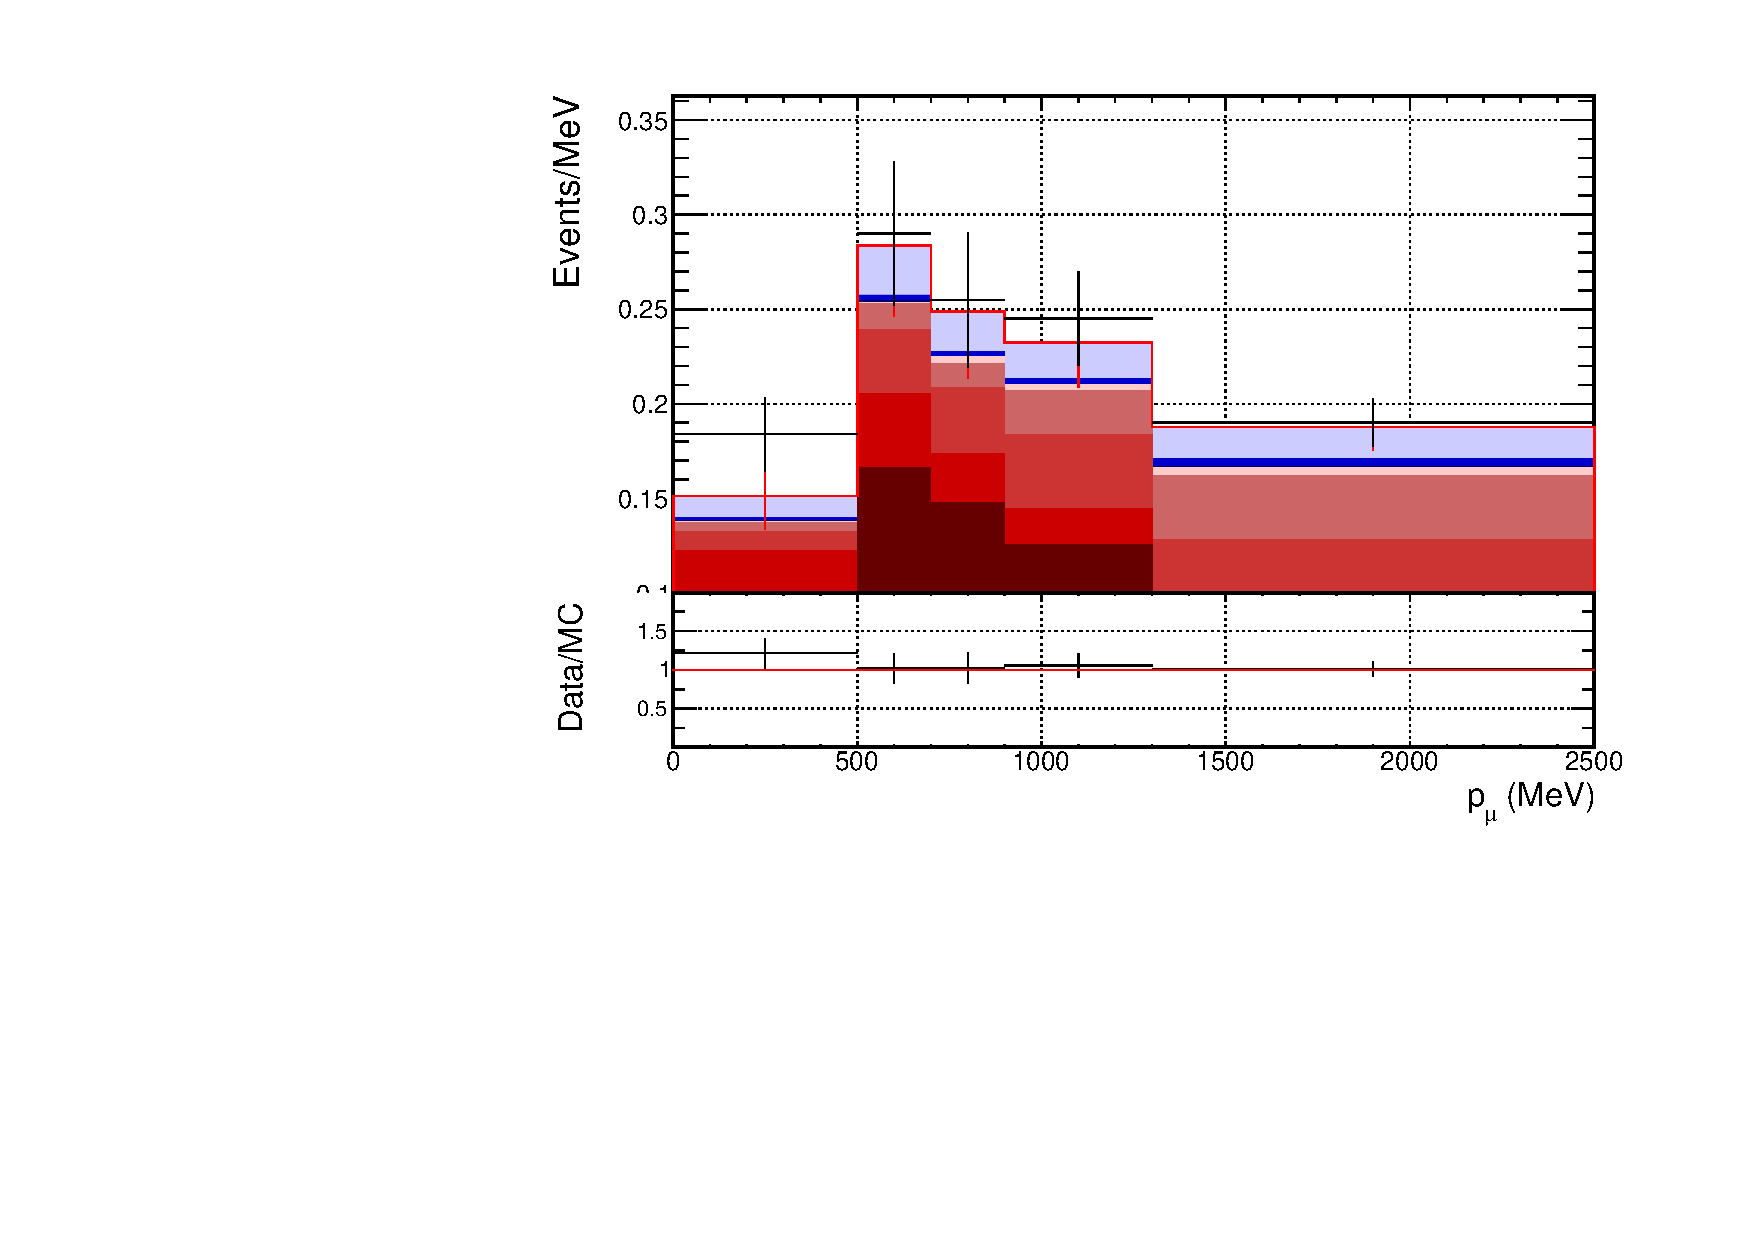
\includegraphics[width=\textwidth]{figs/FGD1_anti-numuCC_1pi_p}
  \caption{FGD1 RHC $\bar{\nu_{\mu}}$ 1$\pi$}
\end{subfigure}
\centering
\begin{subfigure}{0.49\textwidth}
  \centering
  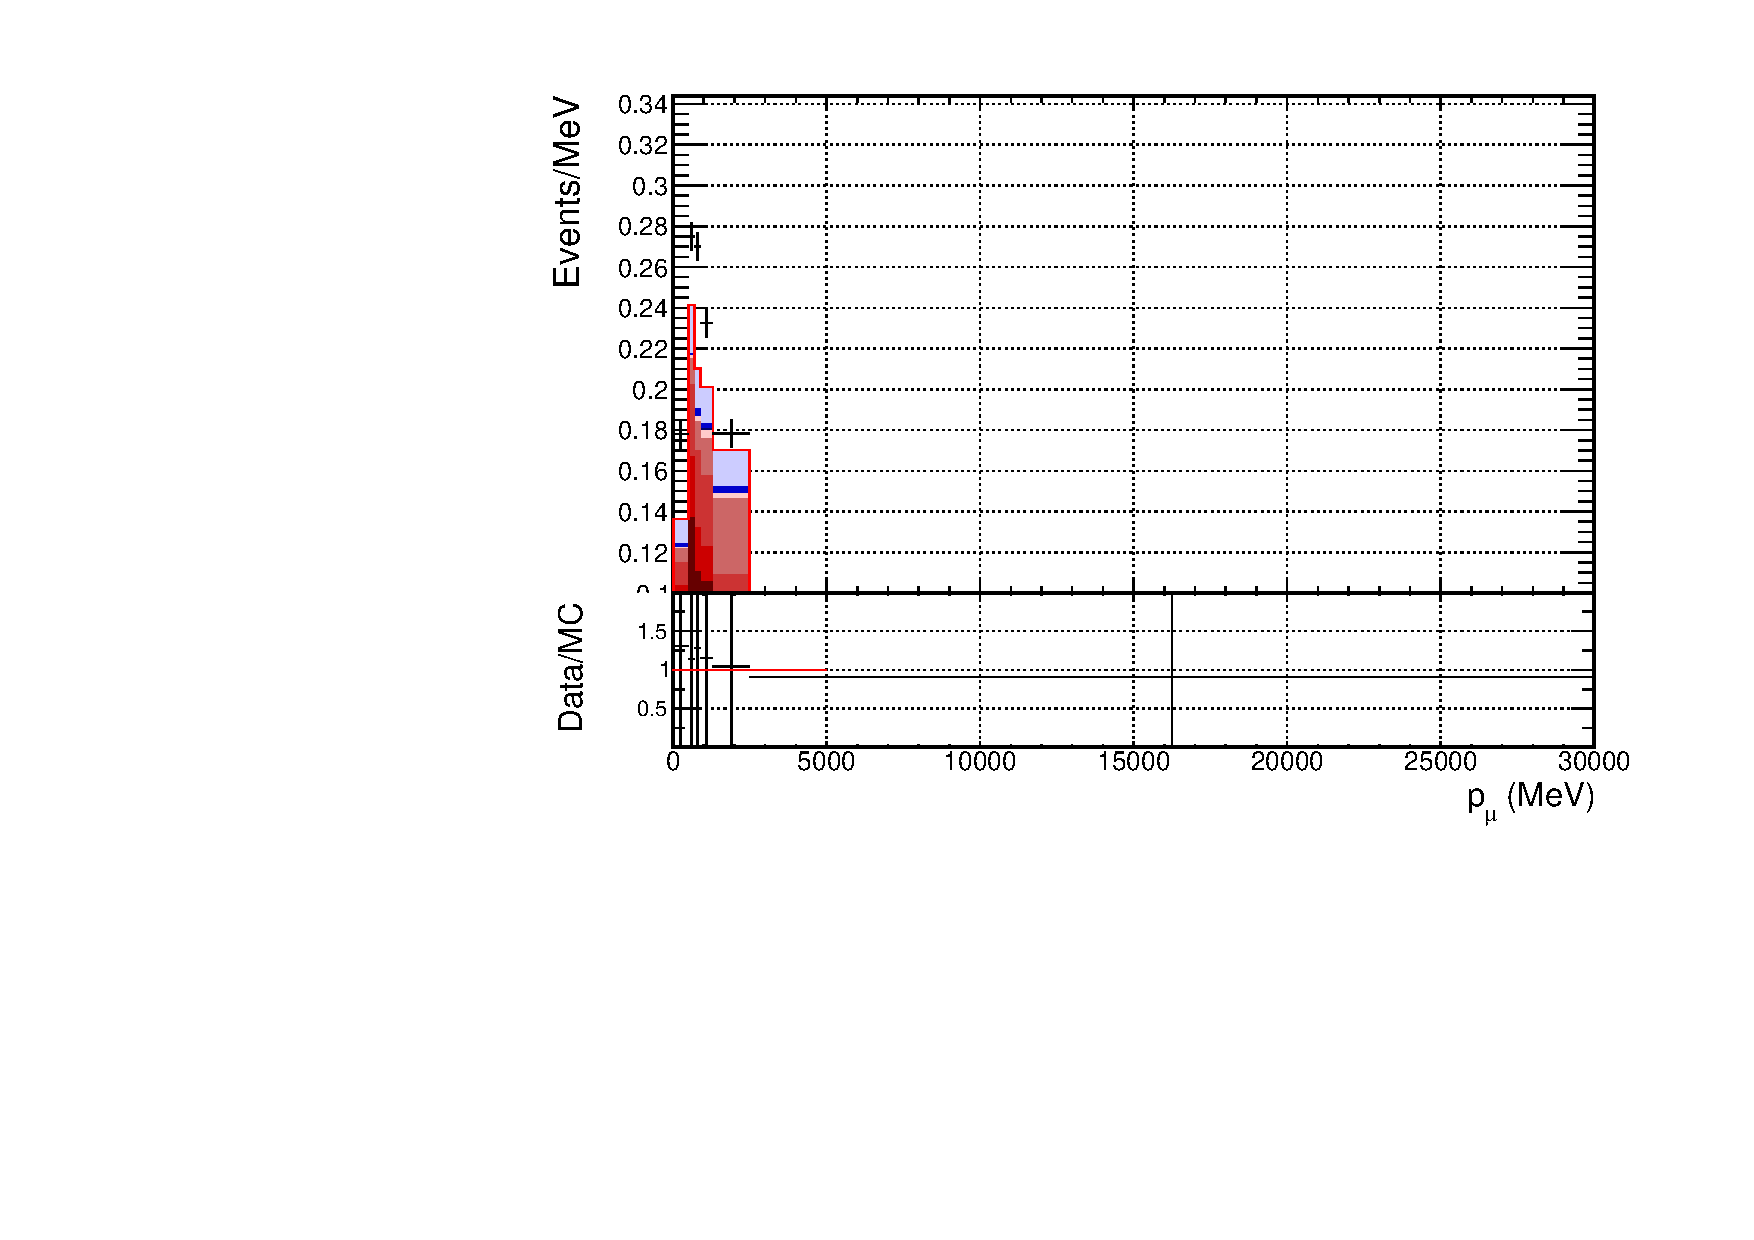
\includegraphics[width=\textwidth]{figs/FGD2_anti-numuCC_1pi_p}
  \caption{FGD2 RHC $\bar{\nu_{\mu}}$ 1$\pi$}
\end{subfigure}

\begin{subfigure}{0.49\textwidth}
  \centering
  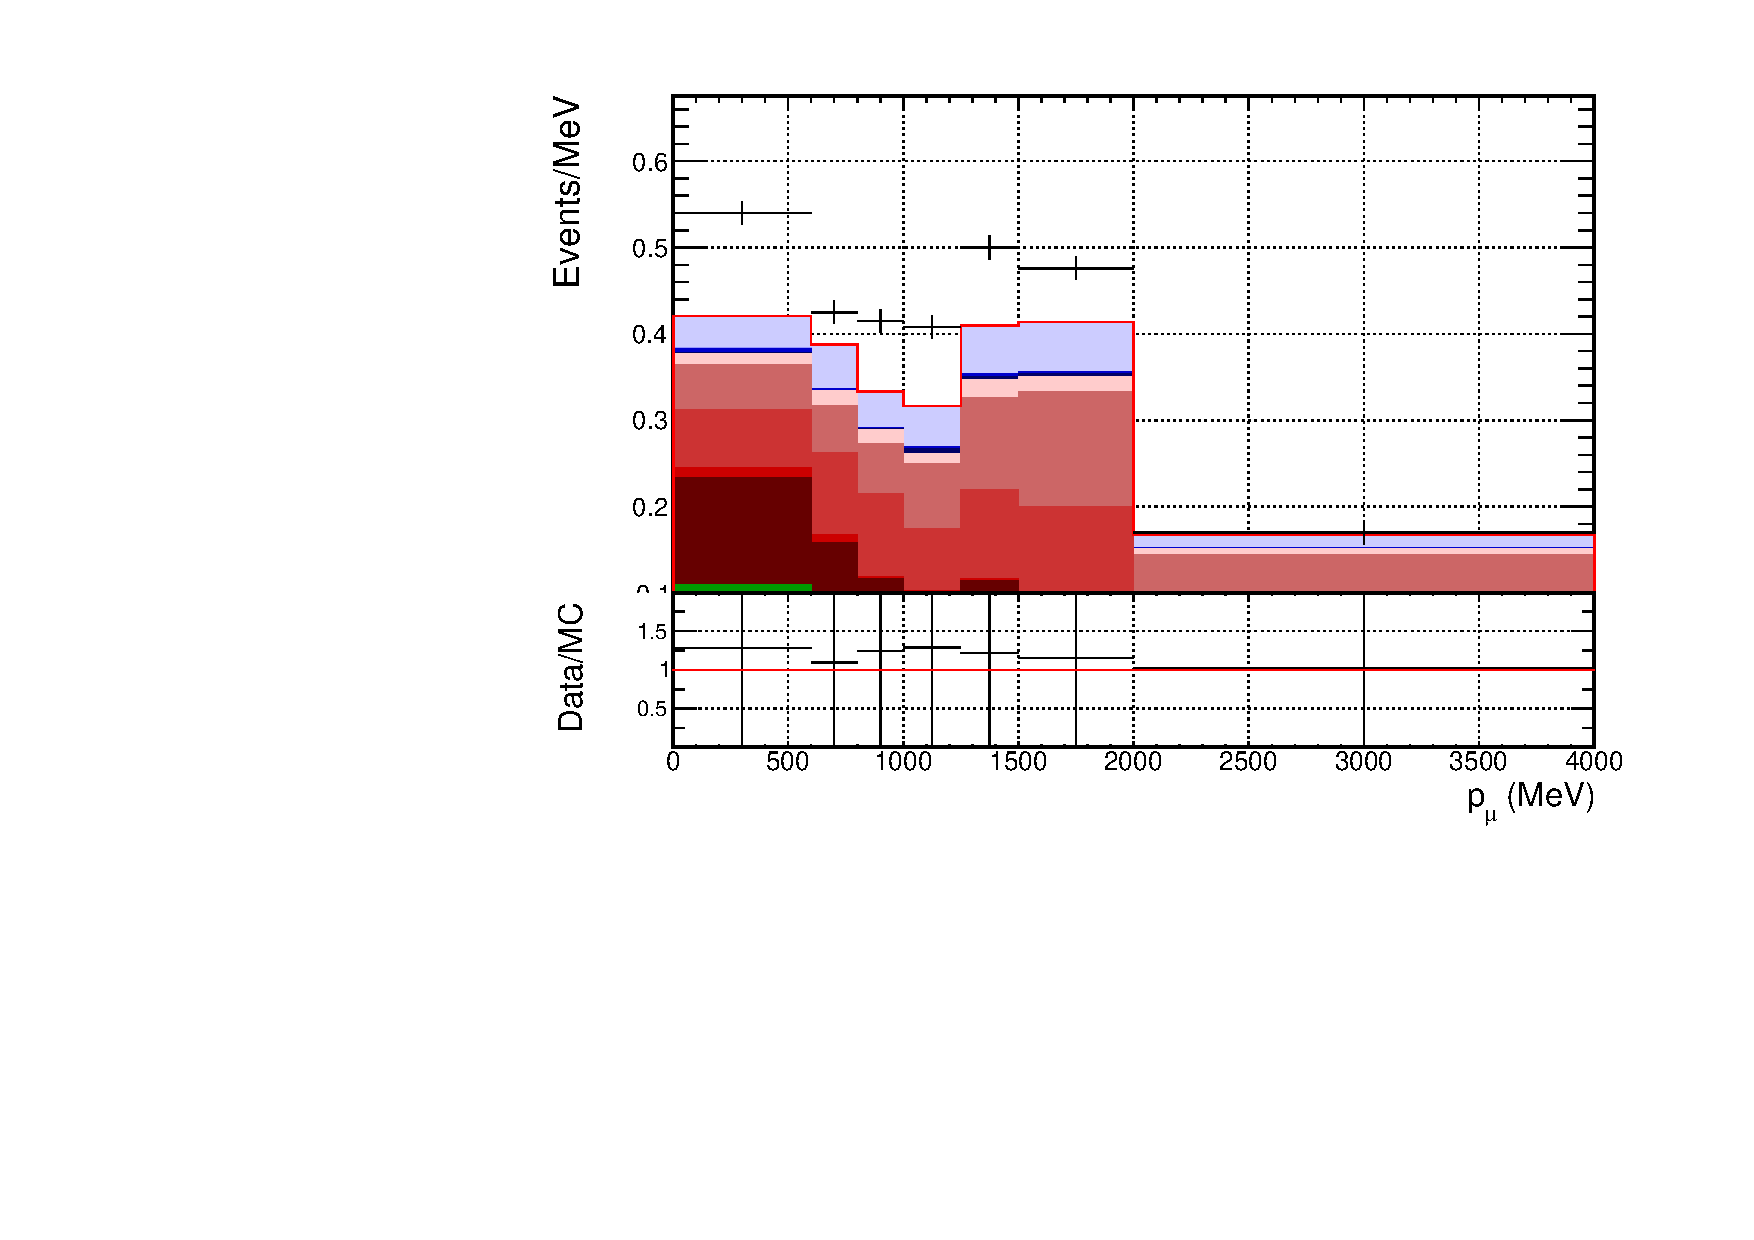
\includegraphics[width=\textwidth]{figs/FGD1_anti-numuCC_other_p}
  \caption{FGD1 RHC $\bar{\nu_{\mu}}$ Other}
\end{subfigure}
\begin{subfigure}{0.49\textwidth}
  \centering
  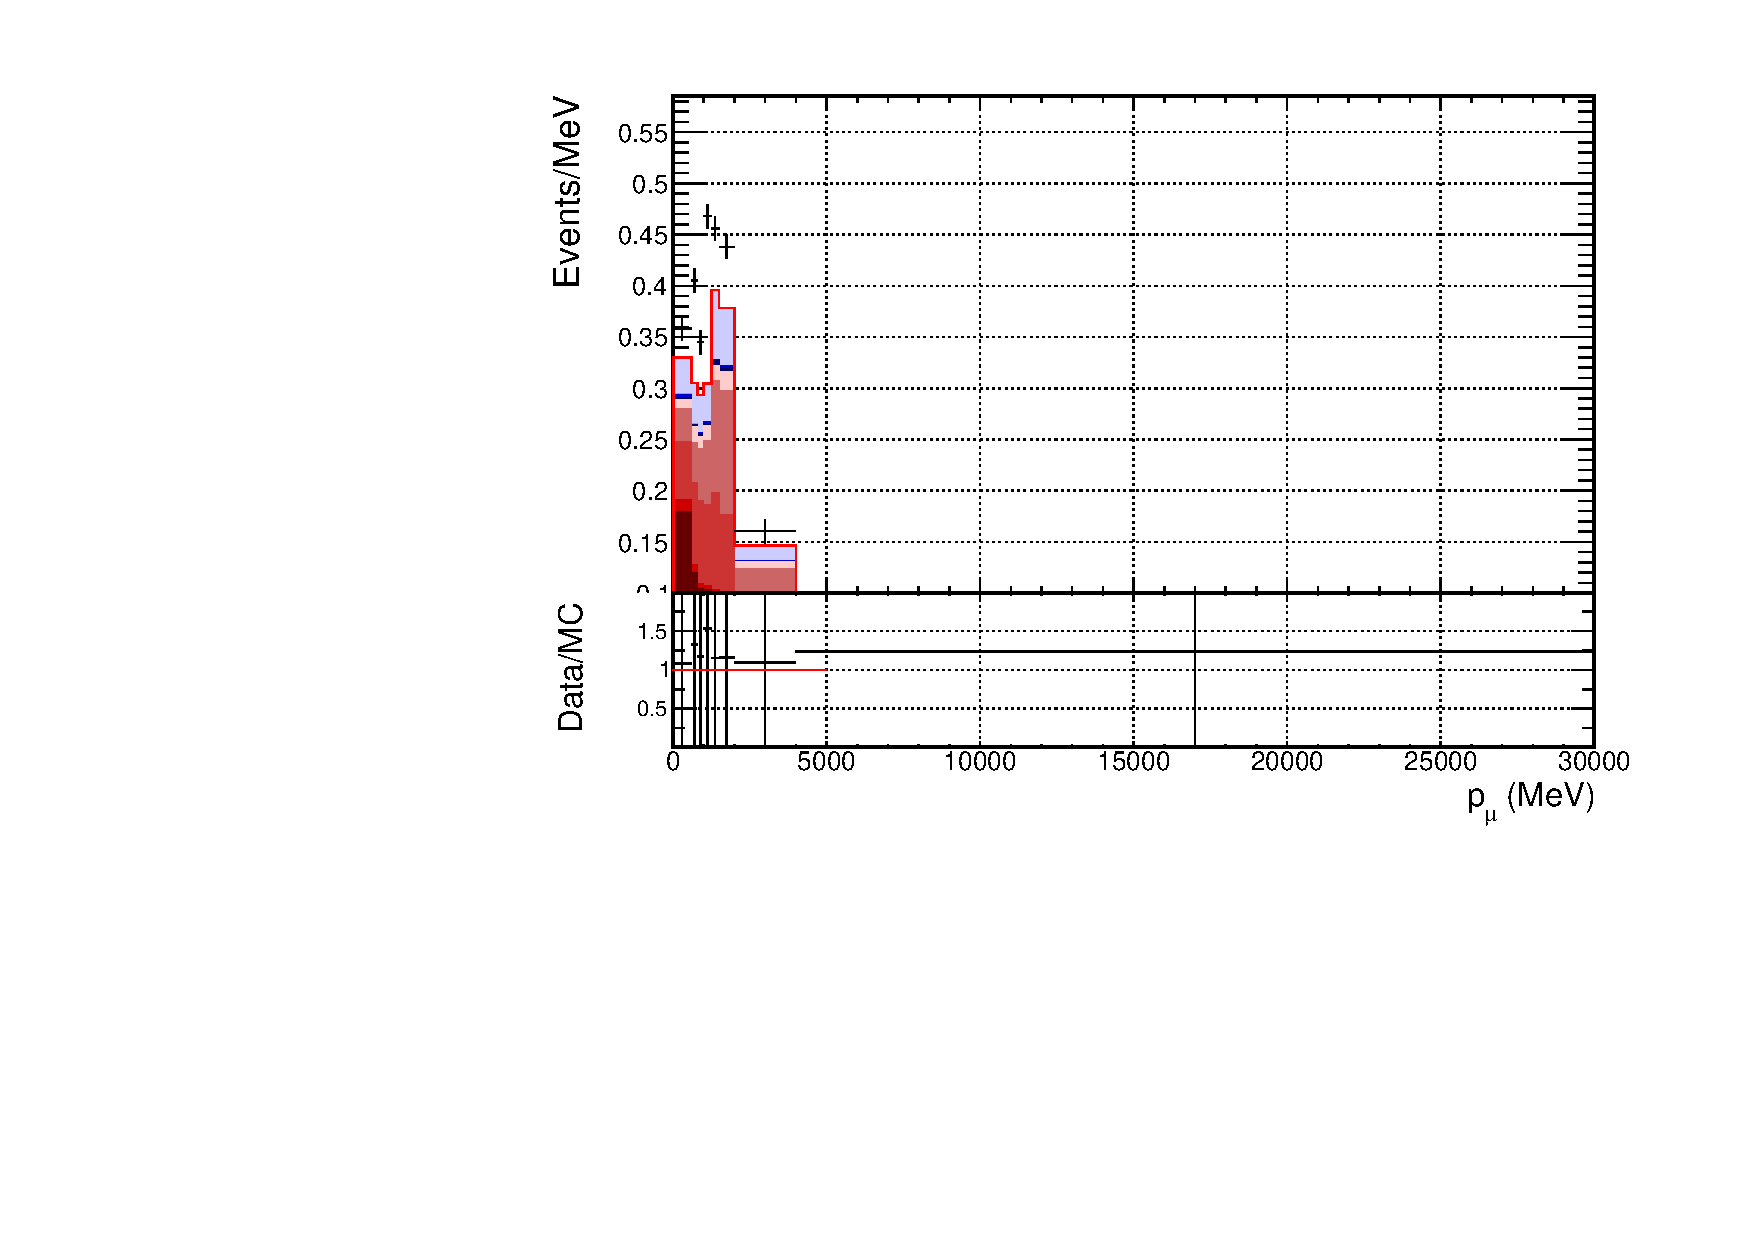
\includegraphics[width=\textwidth]{figs/FGD2_anti-numuCC_other_p}
  \caption{FGD2 RHC $\bar{\nu_{\mu}}$ Other}
\end{subfigure}
\caption{$p_{\mu}$ projections of data and nominal MC broken down by interaction mode for RHC \numub selections.}
\label{fig:pstack_rhc_numubapp}
\end{figure}

\begin{figure}[!htbp]
\centering
\begin{subfigure}{.24\textwidth}
  \centering
  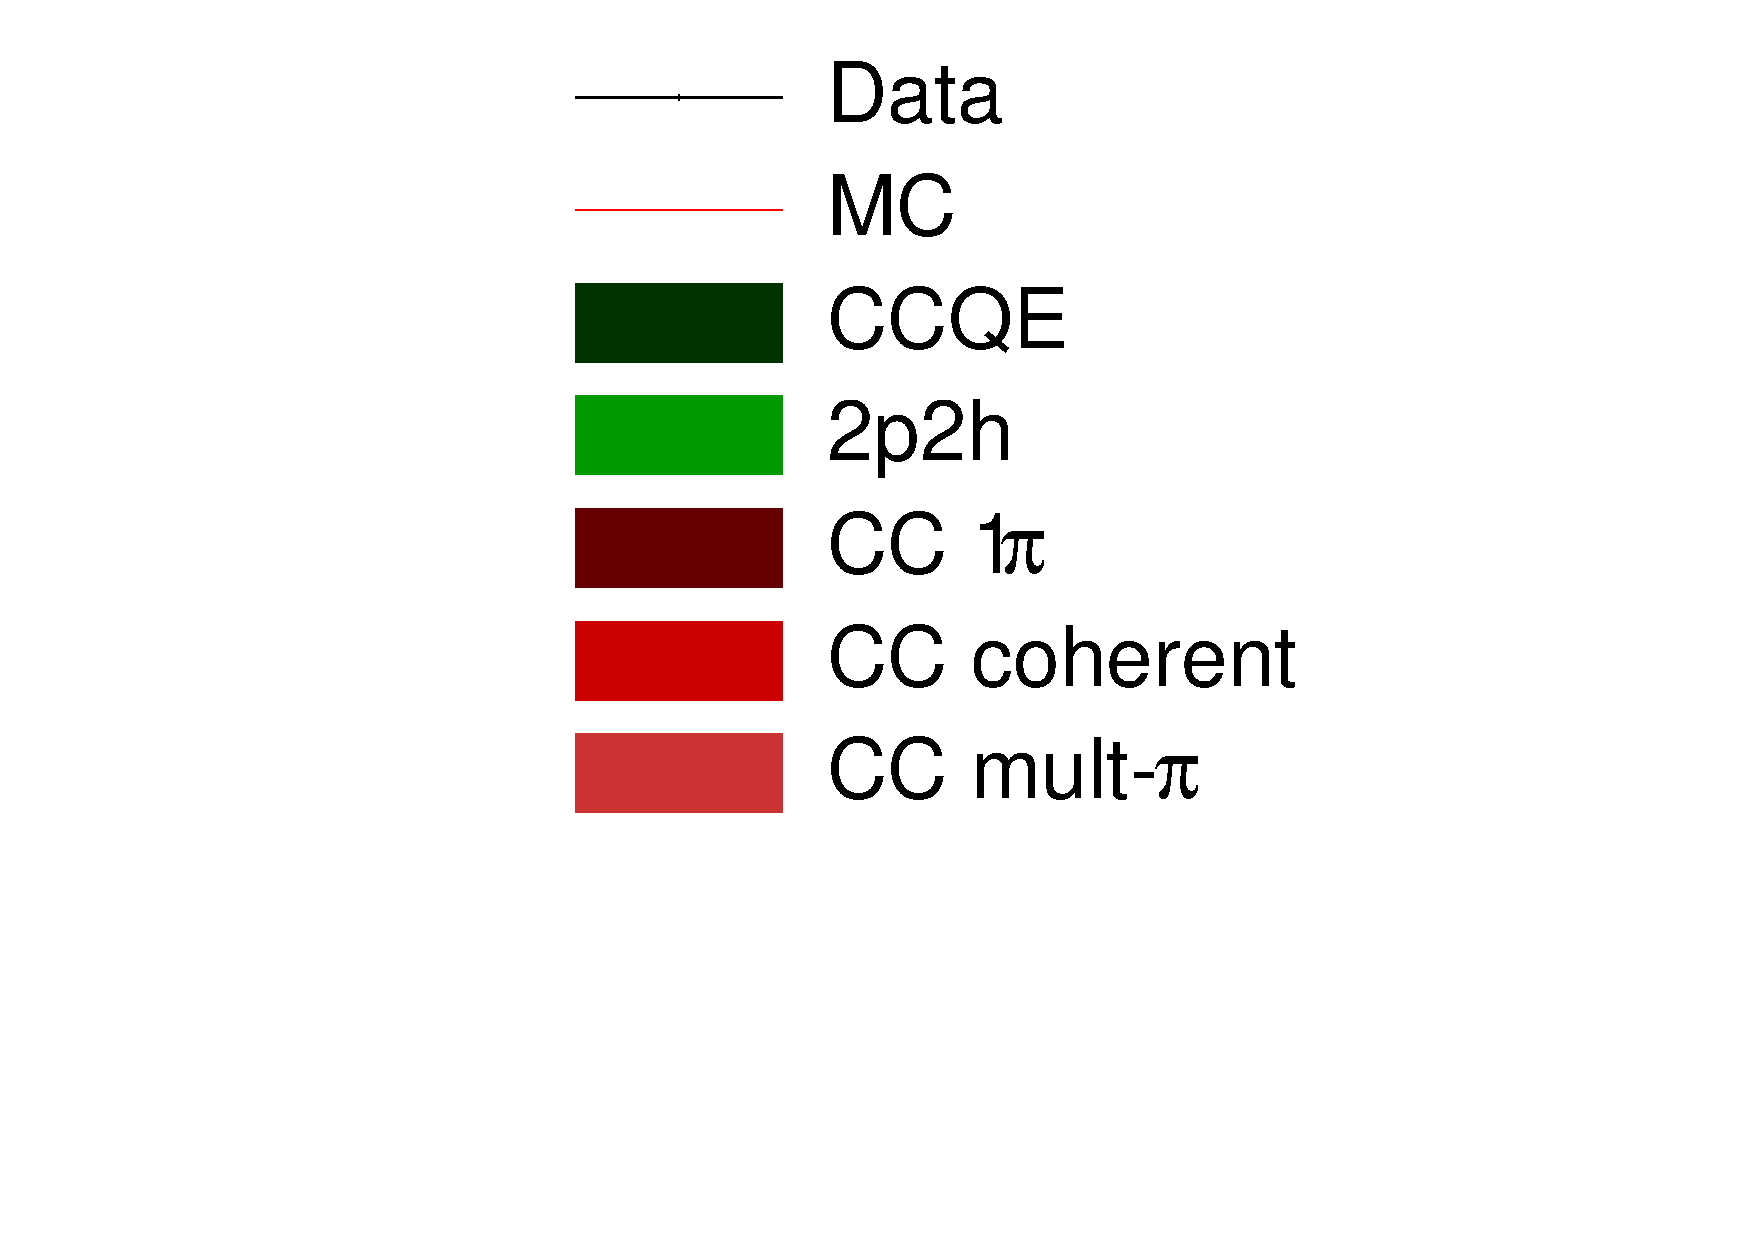
\includegraphics[width=\linewidth, trim={5mm 60mm 30mm 0mm}, clip]{figs/legend}
\end{subfigure}
\begin{subfigure}{.24\textwidth}
  \centering
  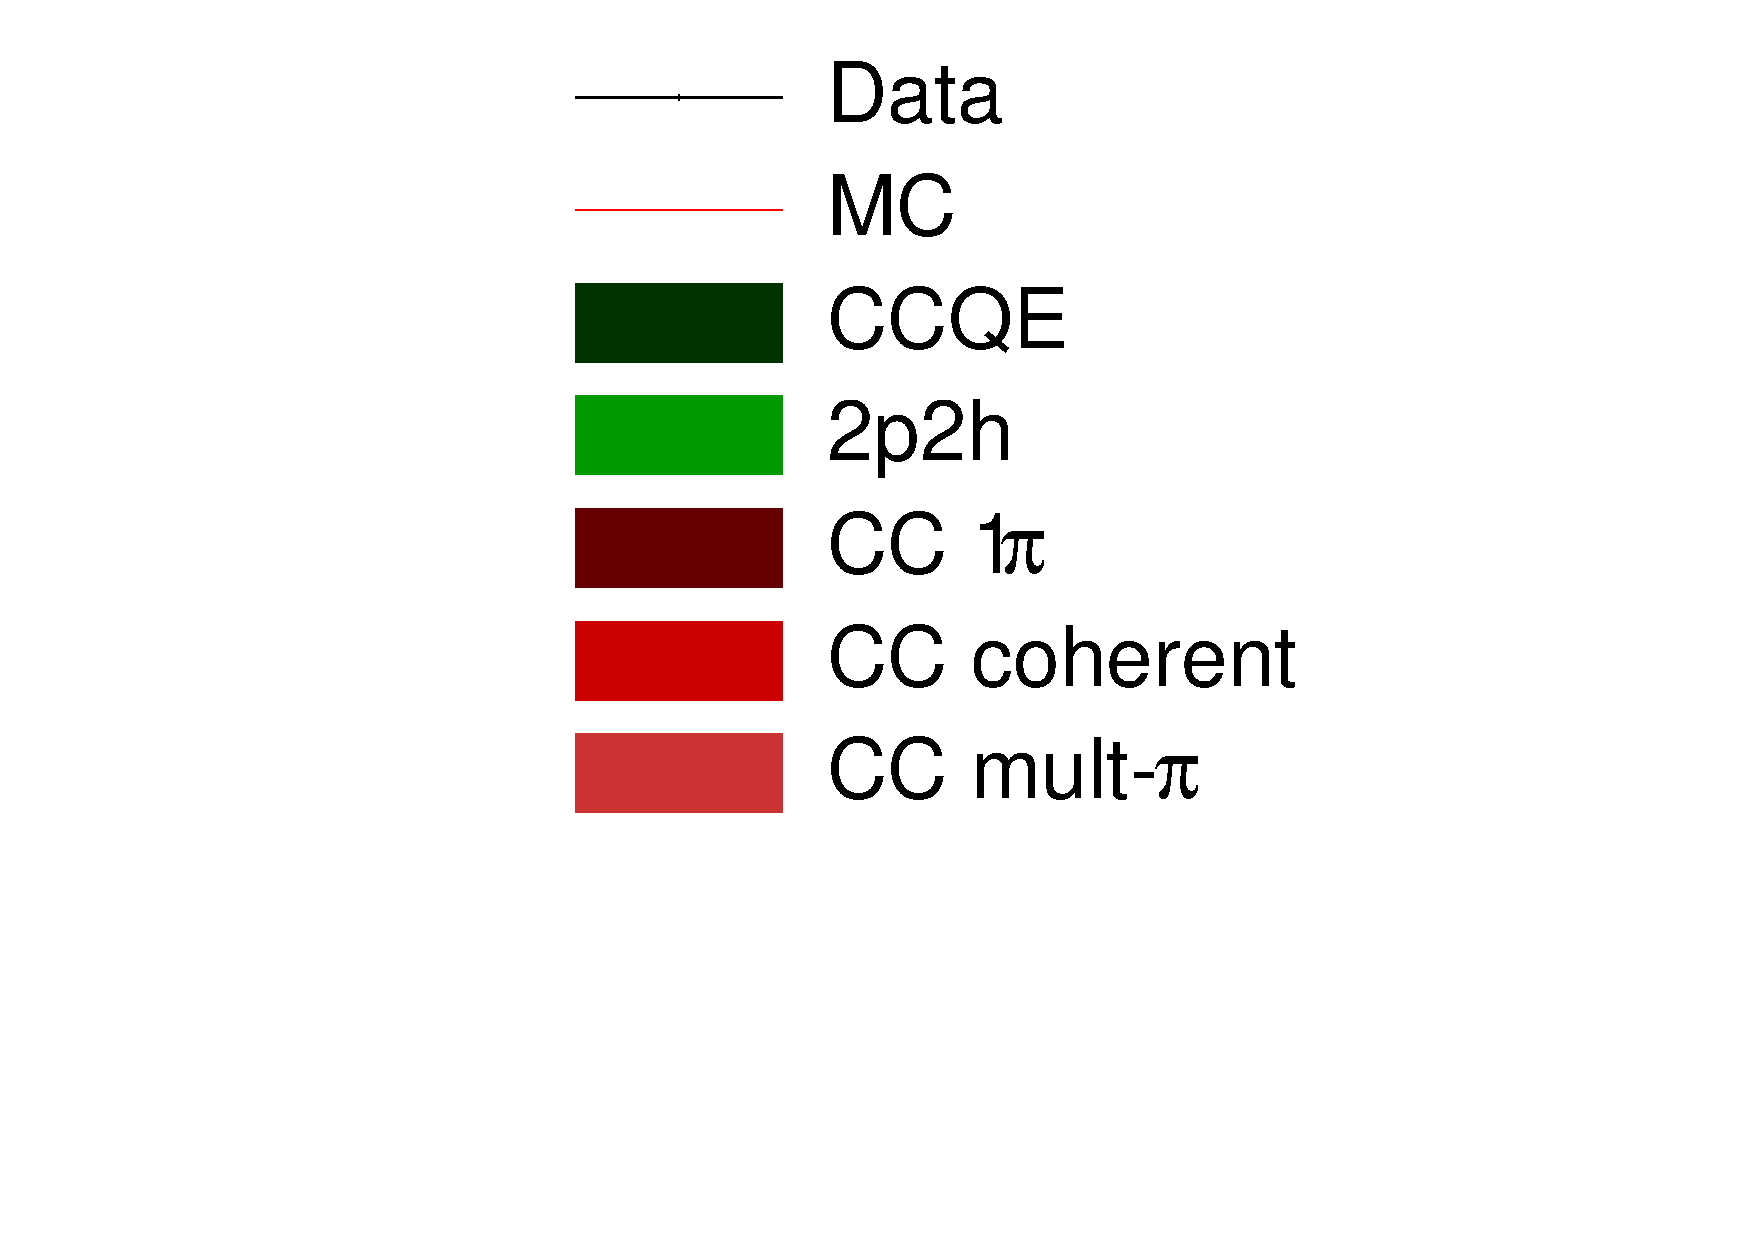
\includegraphics[width=\linewidth, trim={5mm 0mm 30mm 80mm}, clip]{figs/legend}
\end{subfigure}
\begin{subfigure}{.24\textwidth}
  \centering
  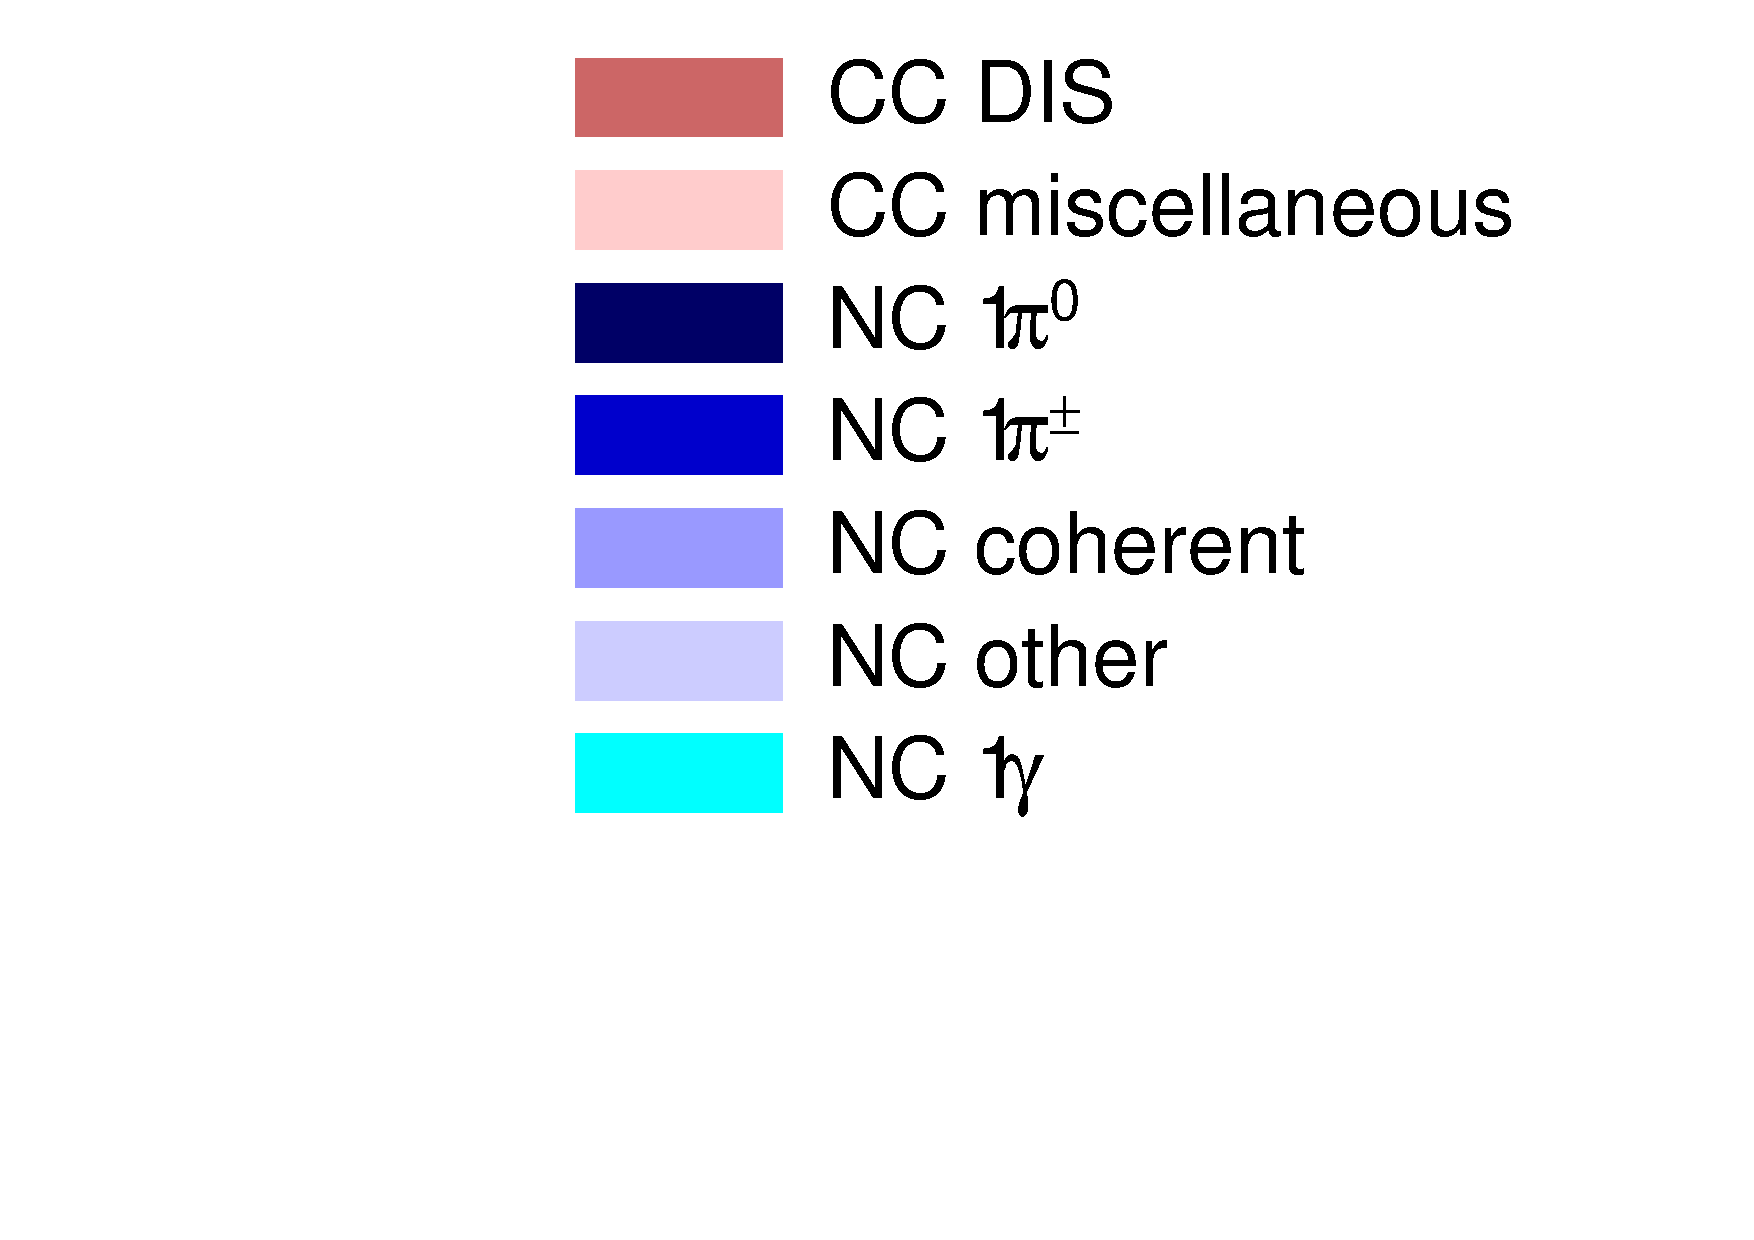
\includegraphics[width=\linewidth, trim={5mm 60mm 30mm 0mm}, clip]{figs/legend2}
\end{subfigure}
\begin{subfigure}{.24\textwidth}
  \centering
  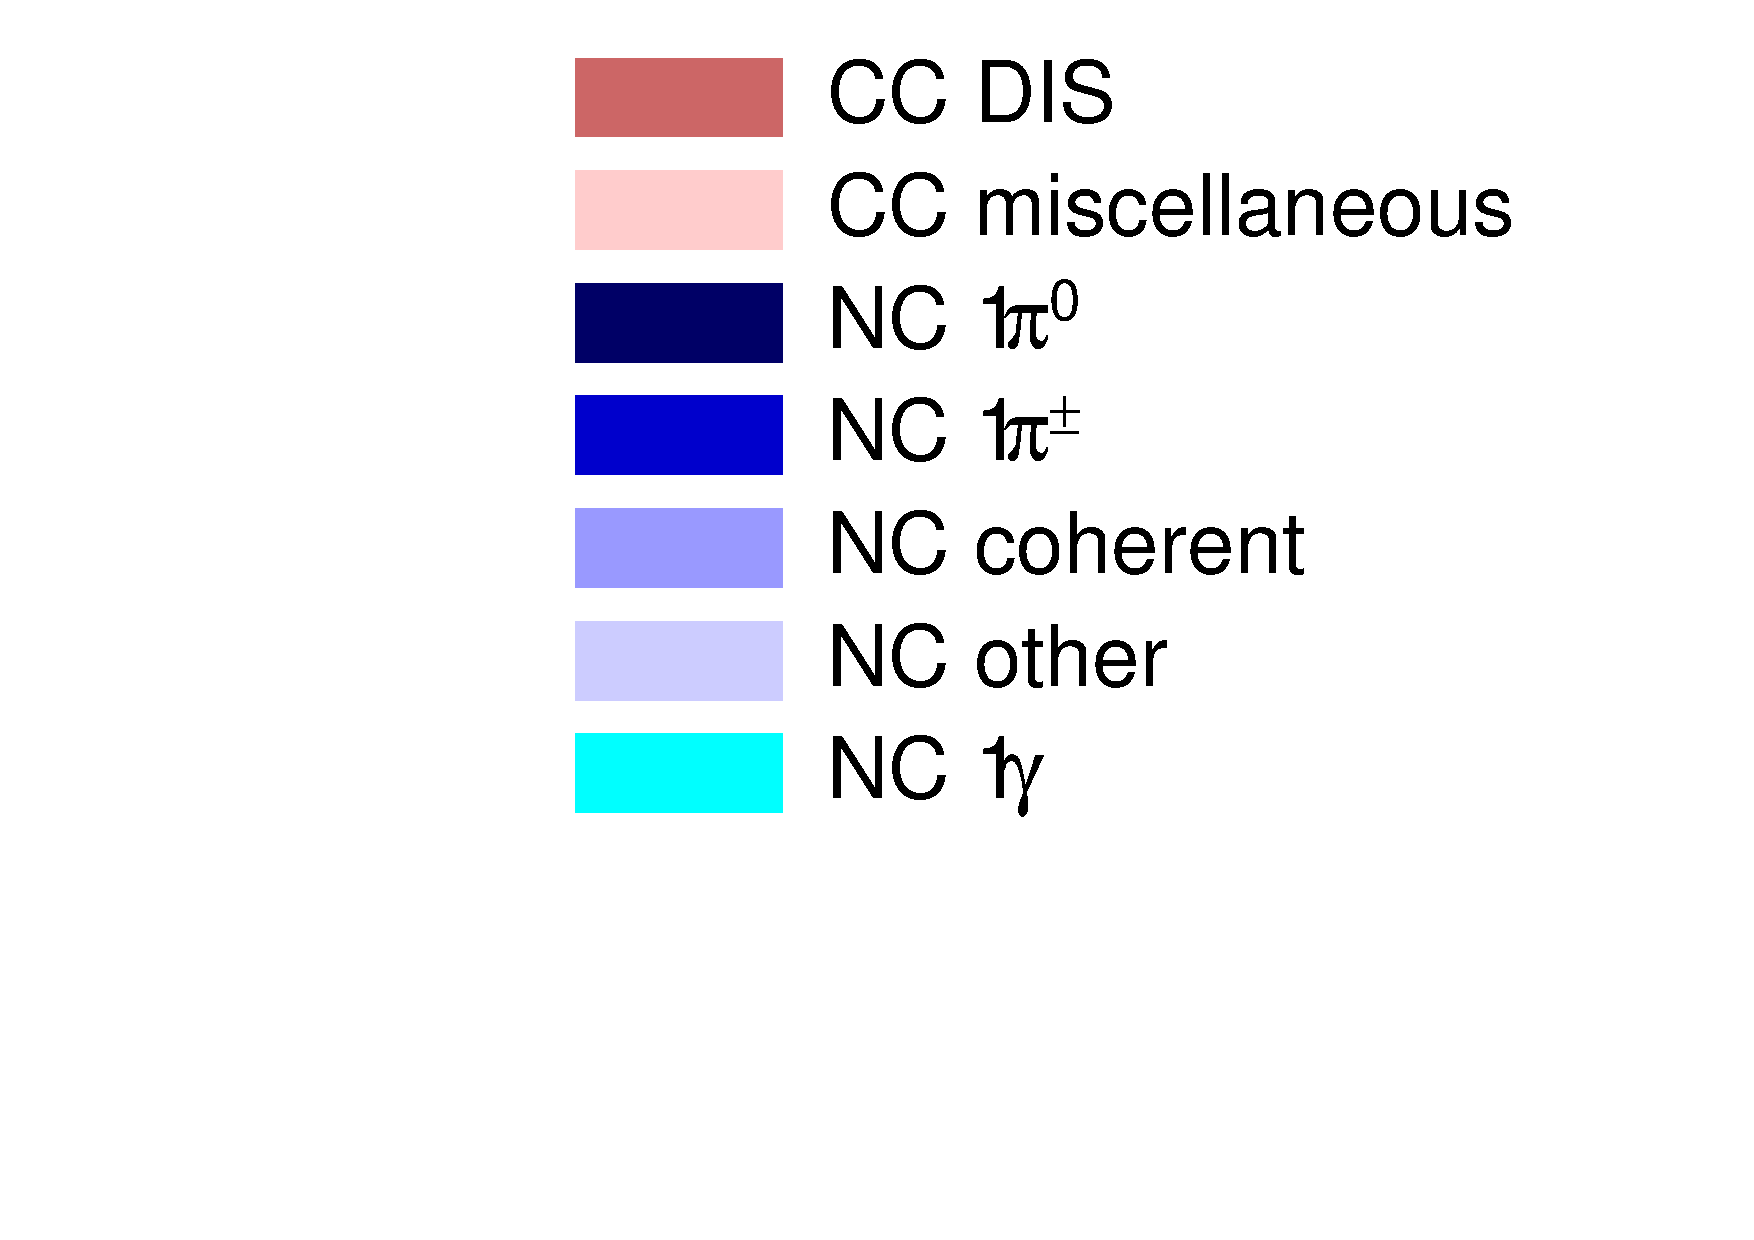
\includegraphics[width=\linewidth, trim={5mm 0mm 30mm 80mm}, clip]{figs/legend2}
\end{subfigure}

\begin{subfigure}{0.49\textwidth}
  \centering
  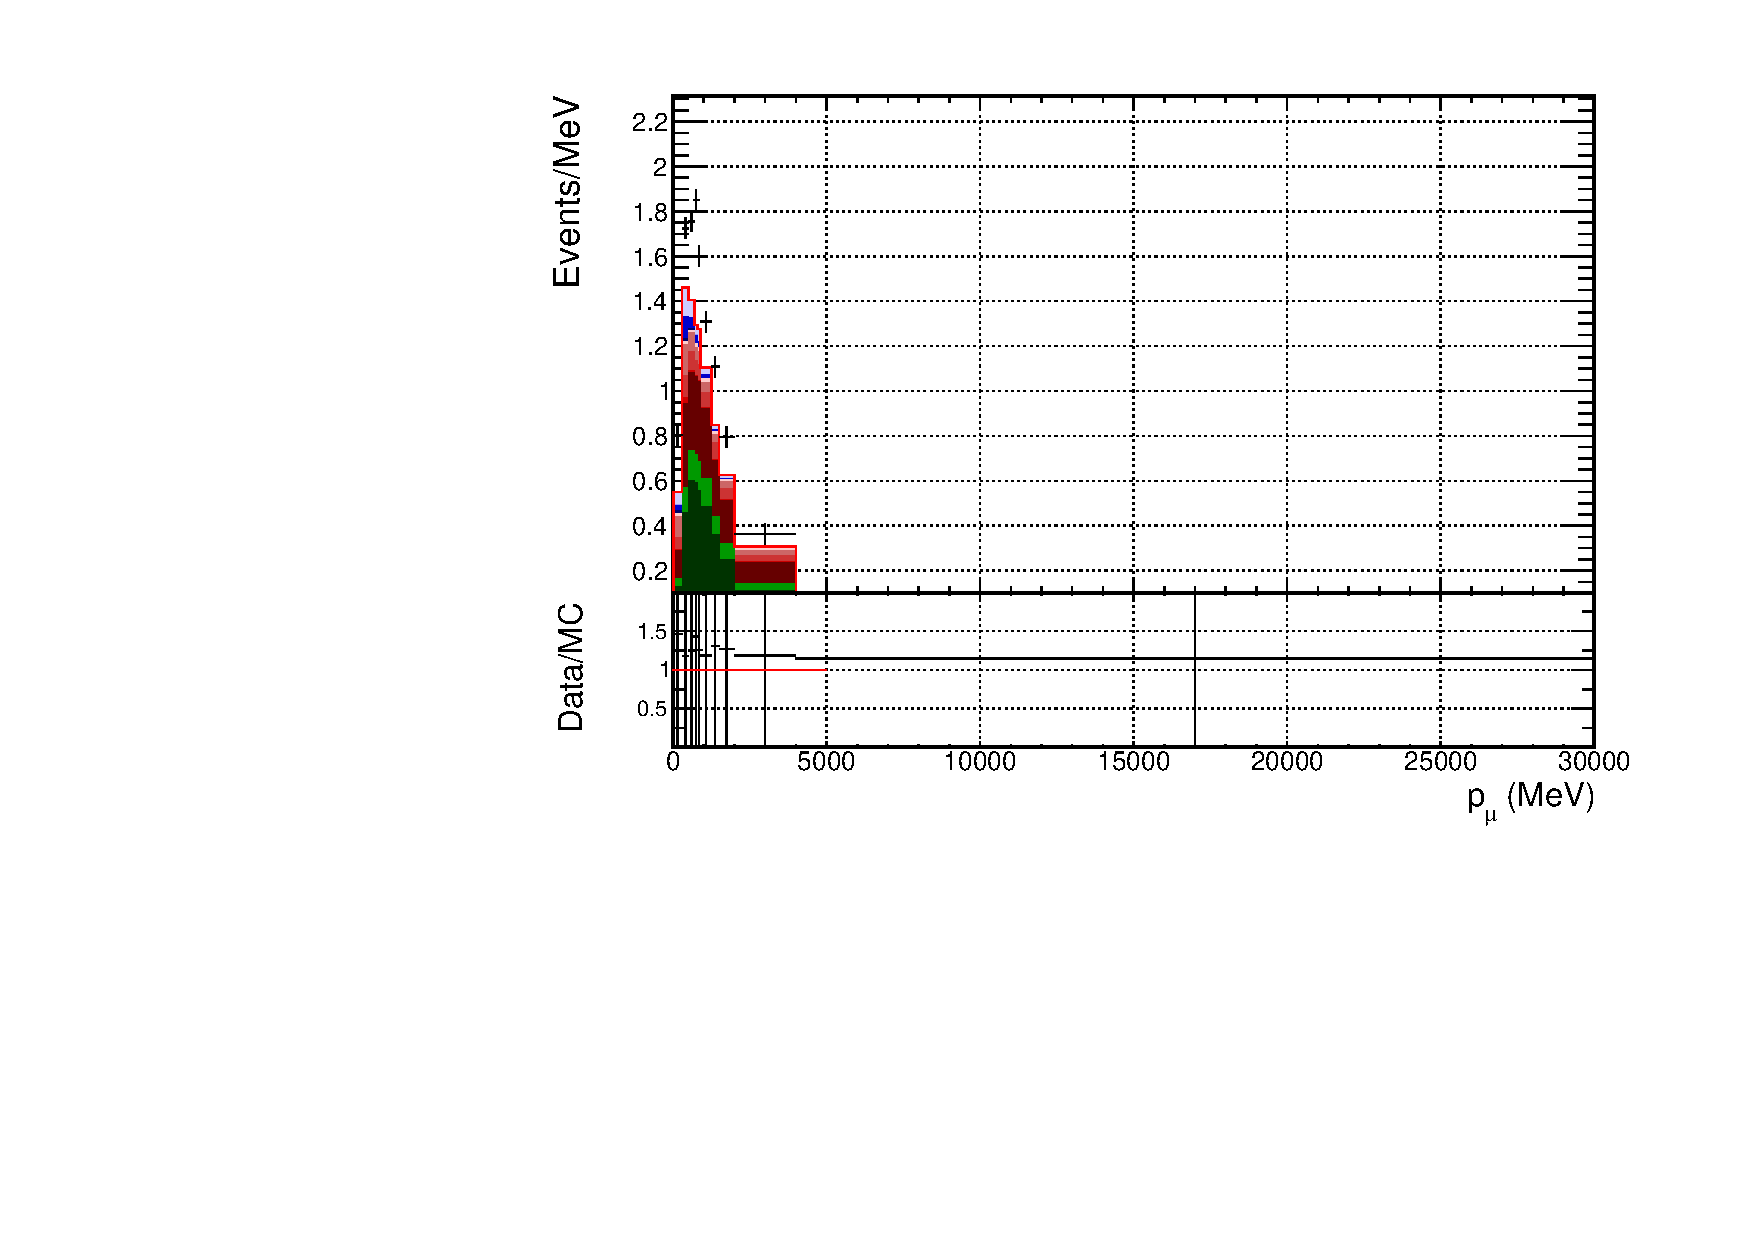
\includegraphics[width=\textwidth]{figs/FGD1_NuMuBkg_CC0pi_in_AntiNu_Mode_p}
  \caption{FGD1 RHC $\nu_{\mu}$ 0$\pi$}
\end{subfigure}
\begin{subfigure}{0.49\textwidth}
  \centering
  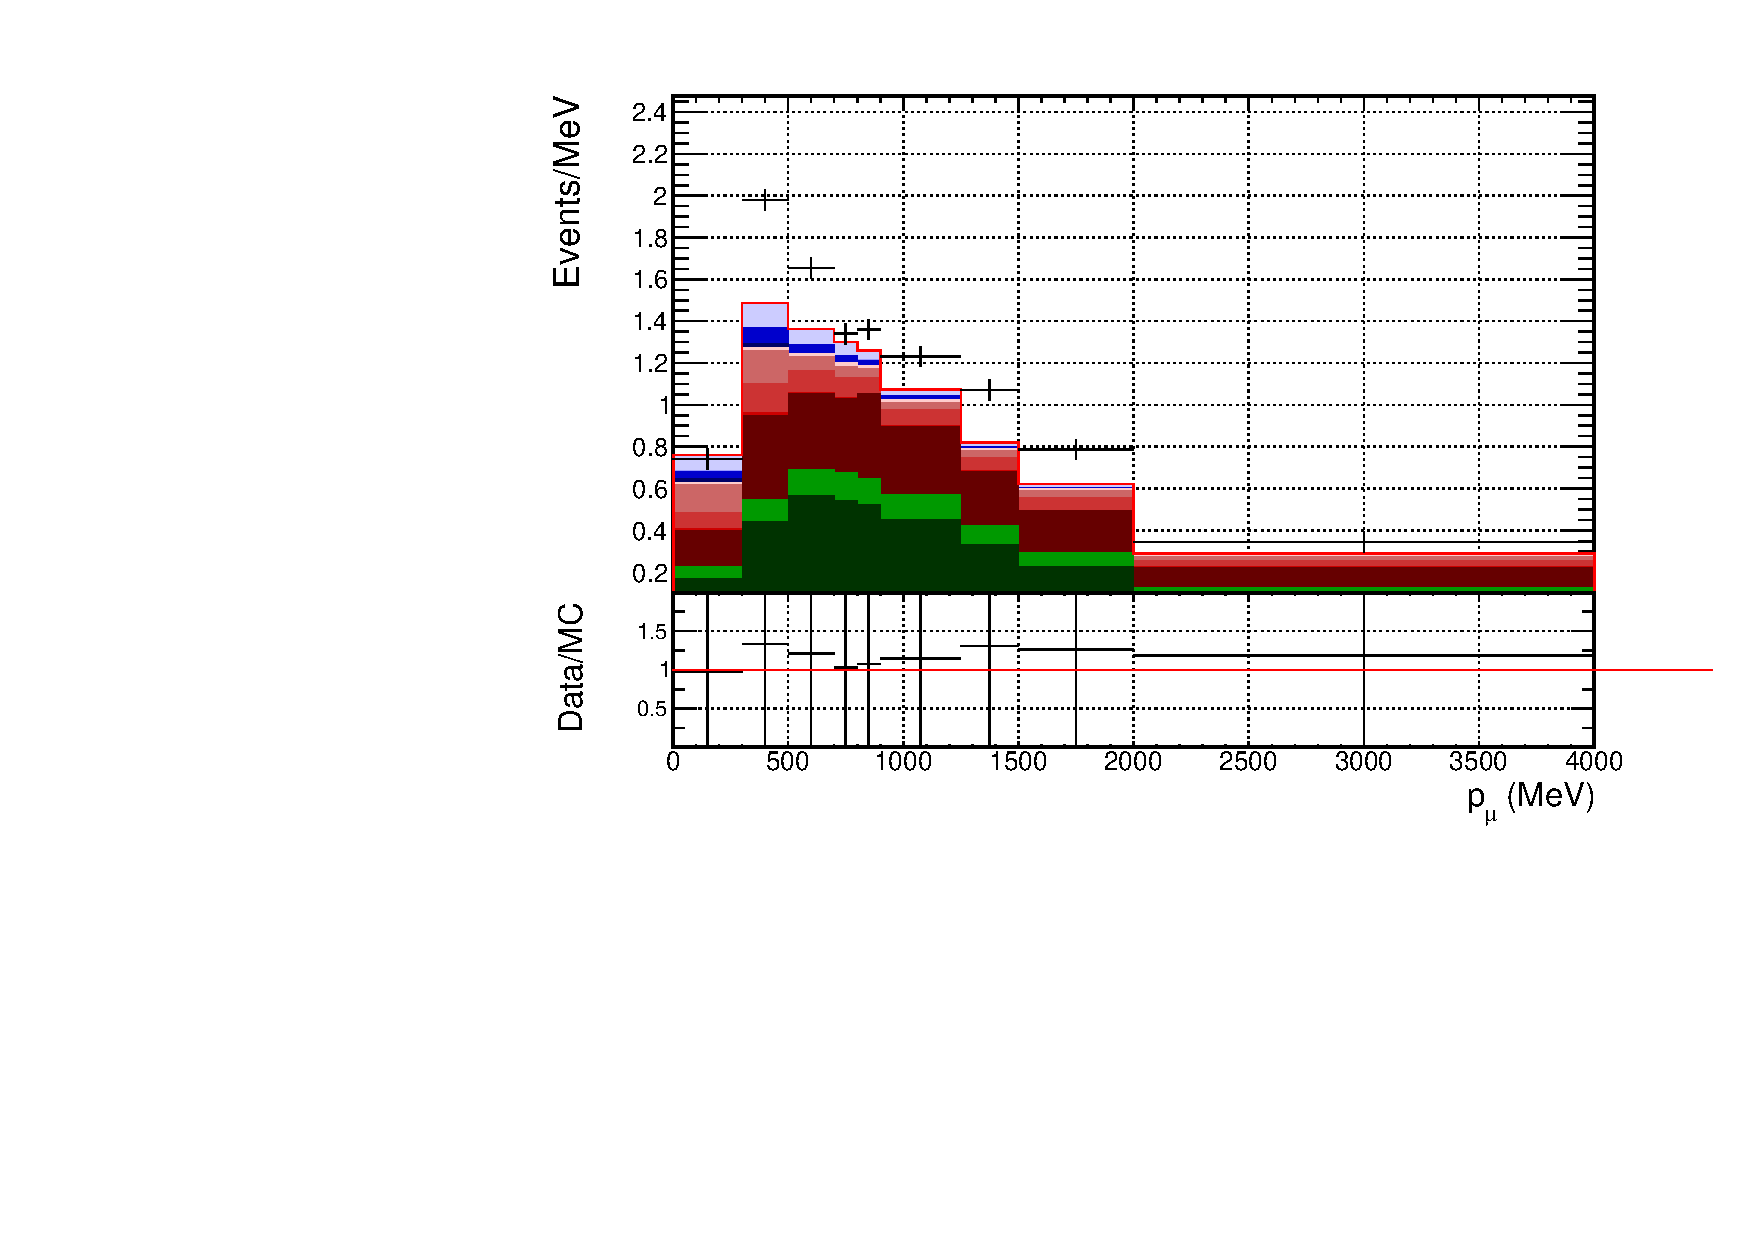
\includegraphics[width=\textwidth]{figs/FGD2_NuMuBkg_CC0pi_in_AntiNu_Mode_p}
  \caption{FGD2 RHC $\nu_{\mu}$ 0$\pi$}
\end{subfigure}

\begin{subfigure}{0.49\textwidth}
  \centering
  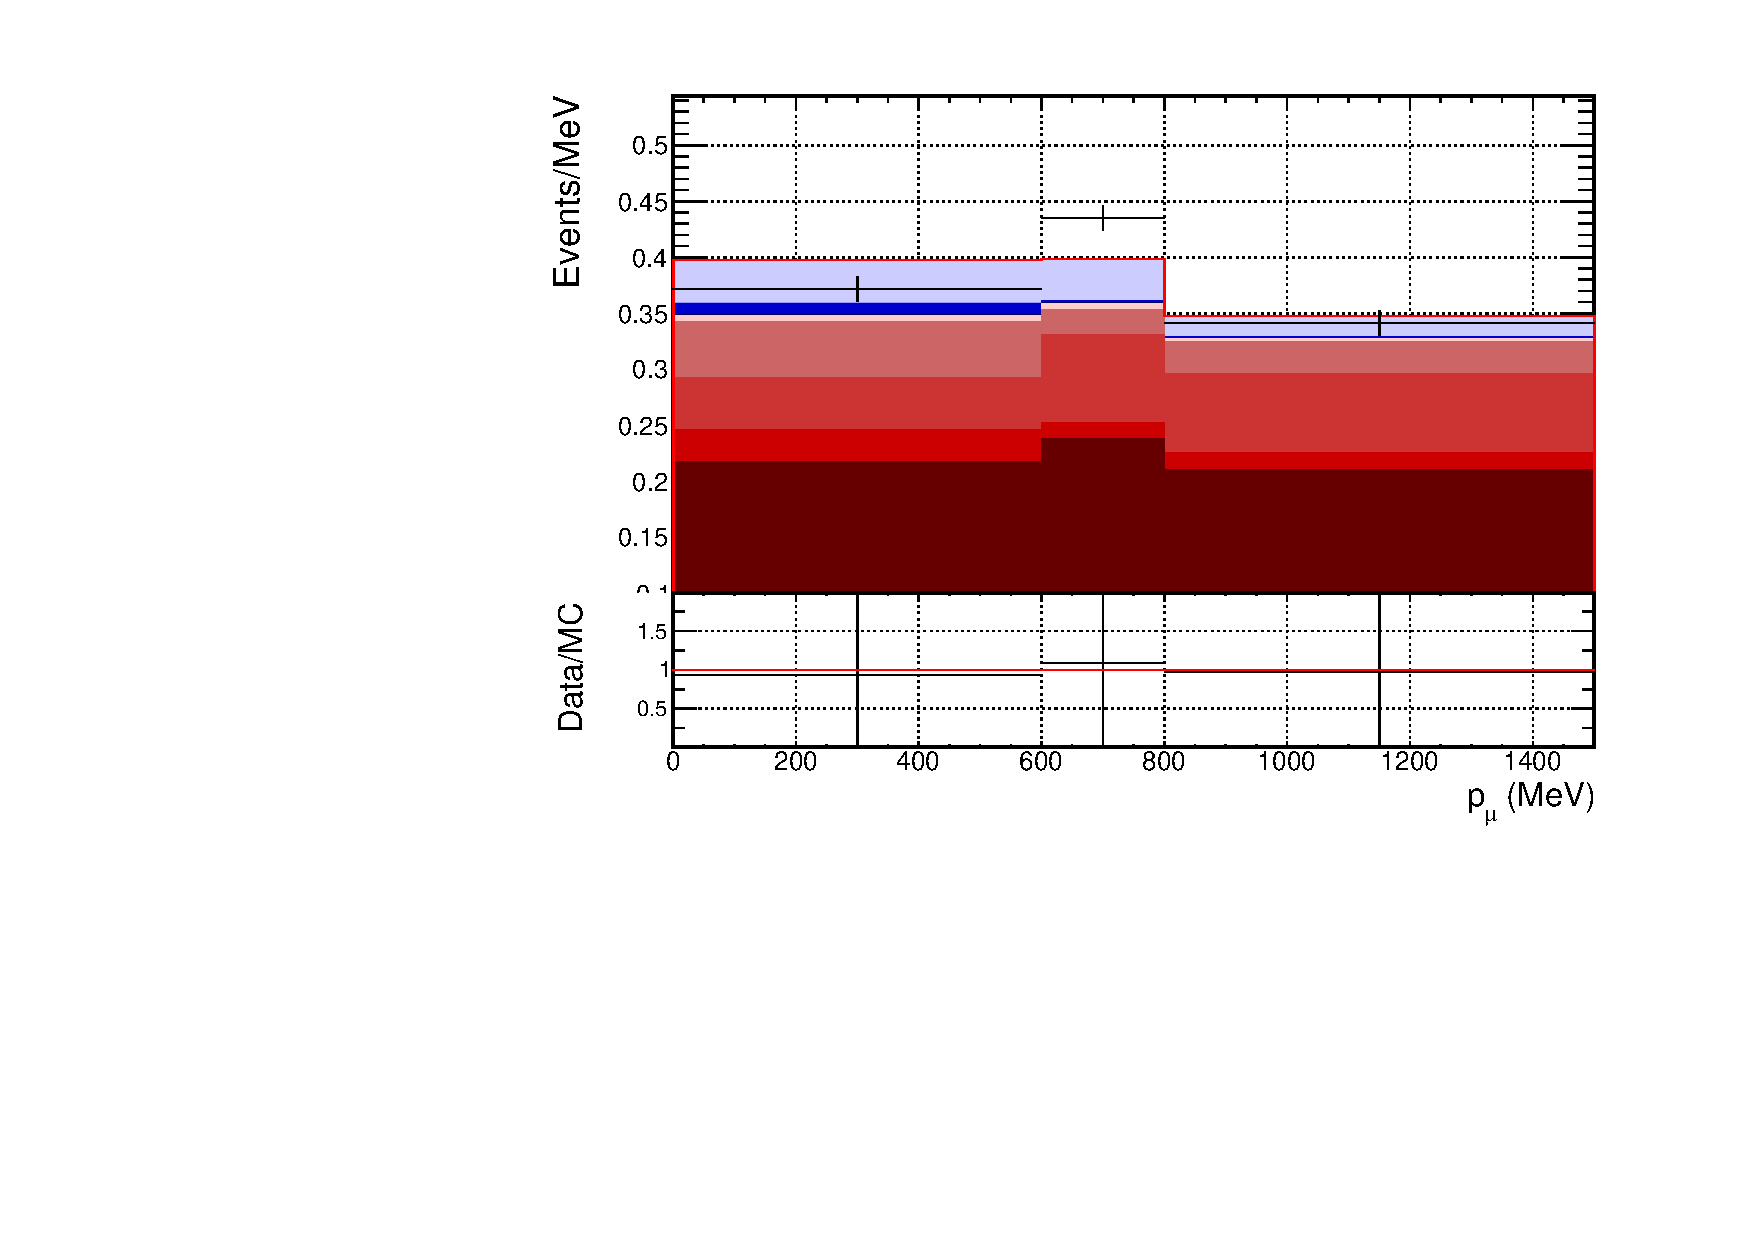
\includegraphics[width=\textwidth]{figs/FGD1_NuMuBkg_CC1pi_in_AntiNu_Mode_p}
  \caption{FGD1 RHC $\nu_{\mu}$ 1$\pi$}
\end{subfigure}
\begin{subfigure}{0.49\textwidth}
  \centering
  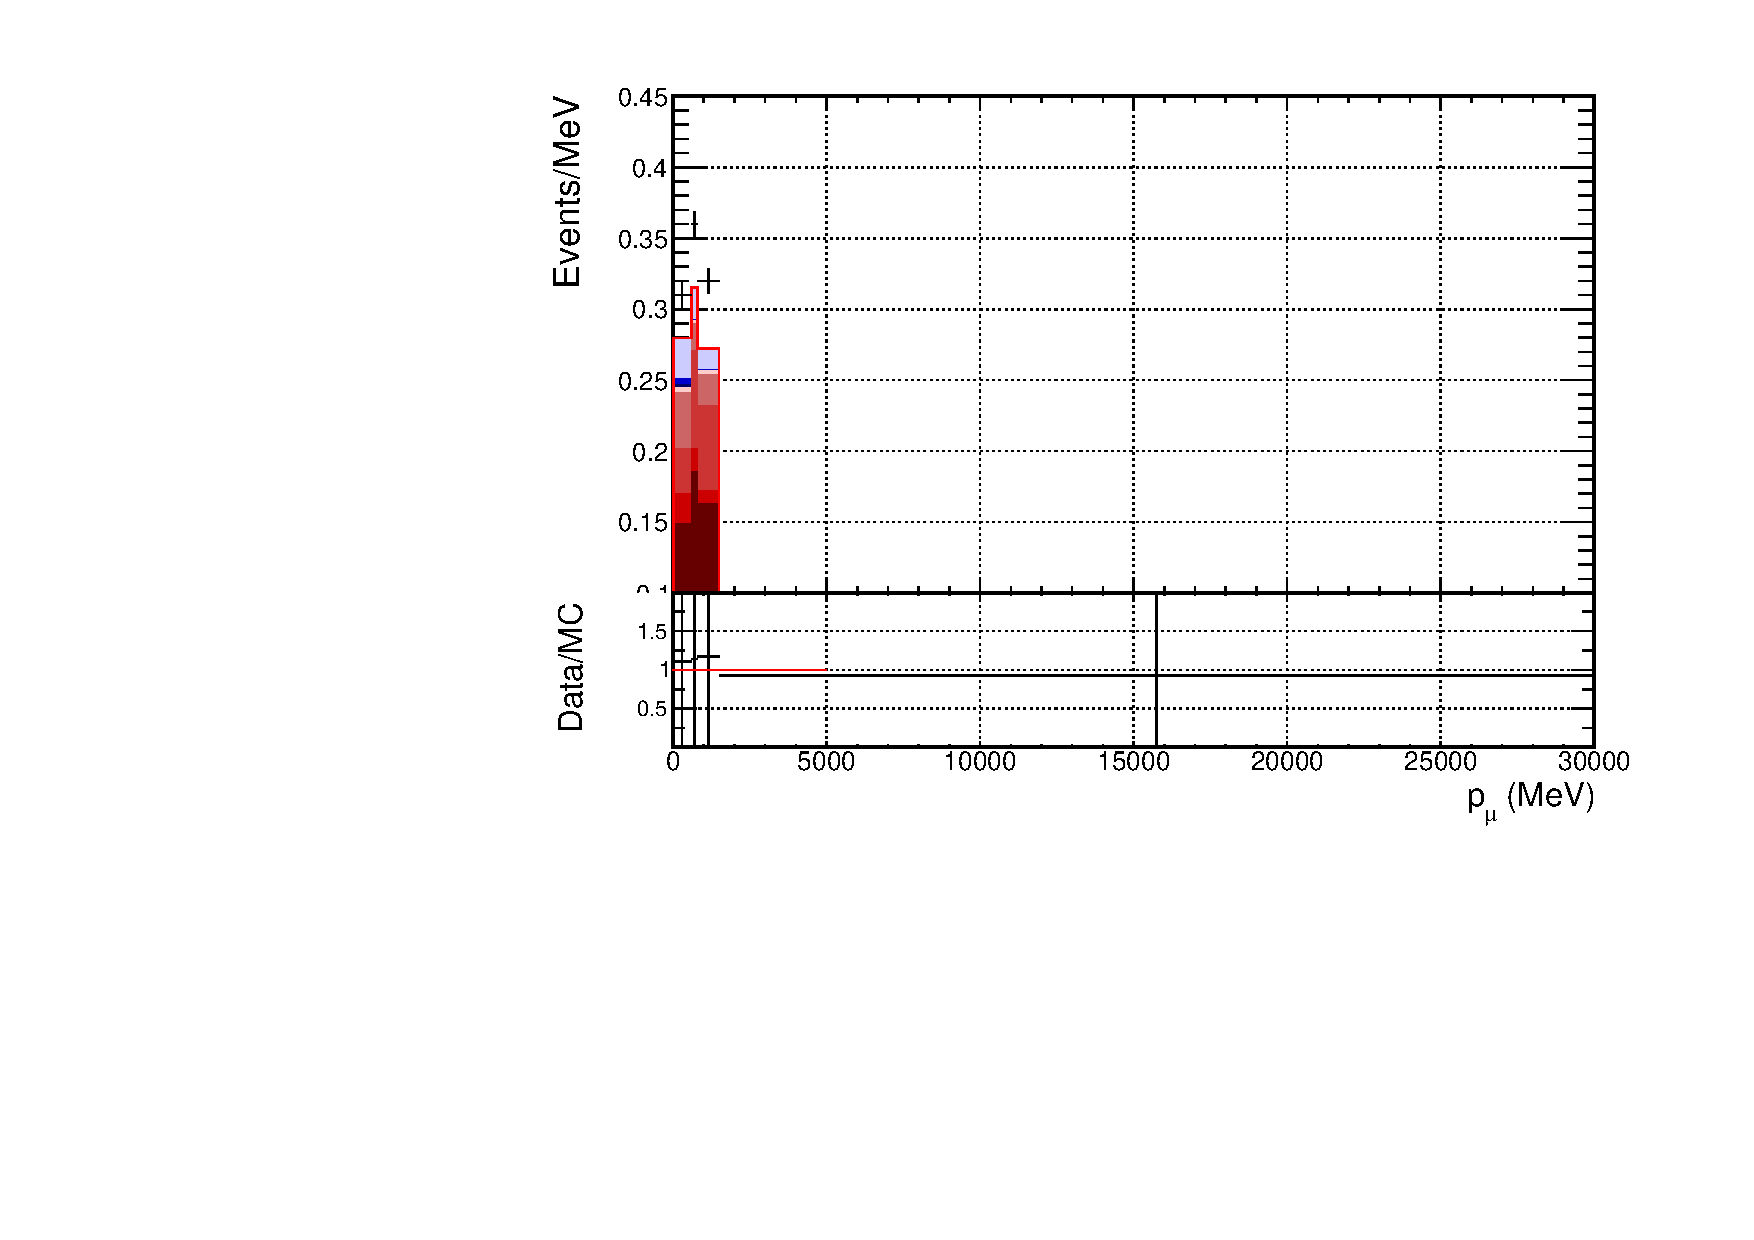
\includegraphics[width=\textwidth]{figs/FGD2_NuMuBkg_CC1pi_in_AntiNu_Mode_p}
  \caption{FGD2 RHC $\nu_{\mu}$ 1$\pi$}
\end{subfigure}

\begin{subfigure}{0.49\textwidth}
  \centering
  \includegraphics[width=\textwidth]{figs/FGD1_NuMuBkg_CCOther_in_AntiNu_Mode_p}
  \caption{FGD1 RHC $\nu_{\mu}$ Other}
\end{subfigure}
\begin{subfigure}{0.49\textwidth}
  \centering
  \includegraphics[width=\textwidth]{figs/FGD2_NuMuBkg_CCOther_in_AntiNu_Mode_p}
  \caption{FGD2 RHC $\nu_{\mu}$ Other}
\end{subfigure}
\caption{$p_{\mu}$ projections of data and nominal MC broken down by interaction mode for RHC \numu selections.}
\label{fig:pstack_rhc_numuapp}
\end{figure}

The projection of the non-uniformly binned nominal MC distributions onto the cos$\theta_{\mu}$ axis are shown in Figures \ref{fig:tstack_fhcapp}, \ref{fig:tstack_rhc_numubapp}, and \ref{fig:tstack_rhc_numuapp}, along with the interaction mode breakdown and data.

\begin{figure}[!htbp]
\centering
\begin{subfigure}{.24\textwidth}
  \centering
  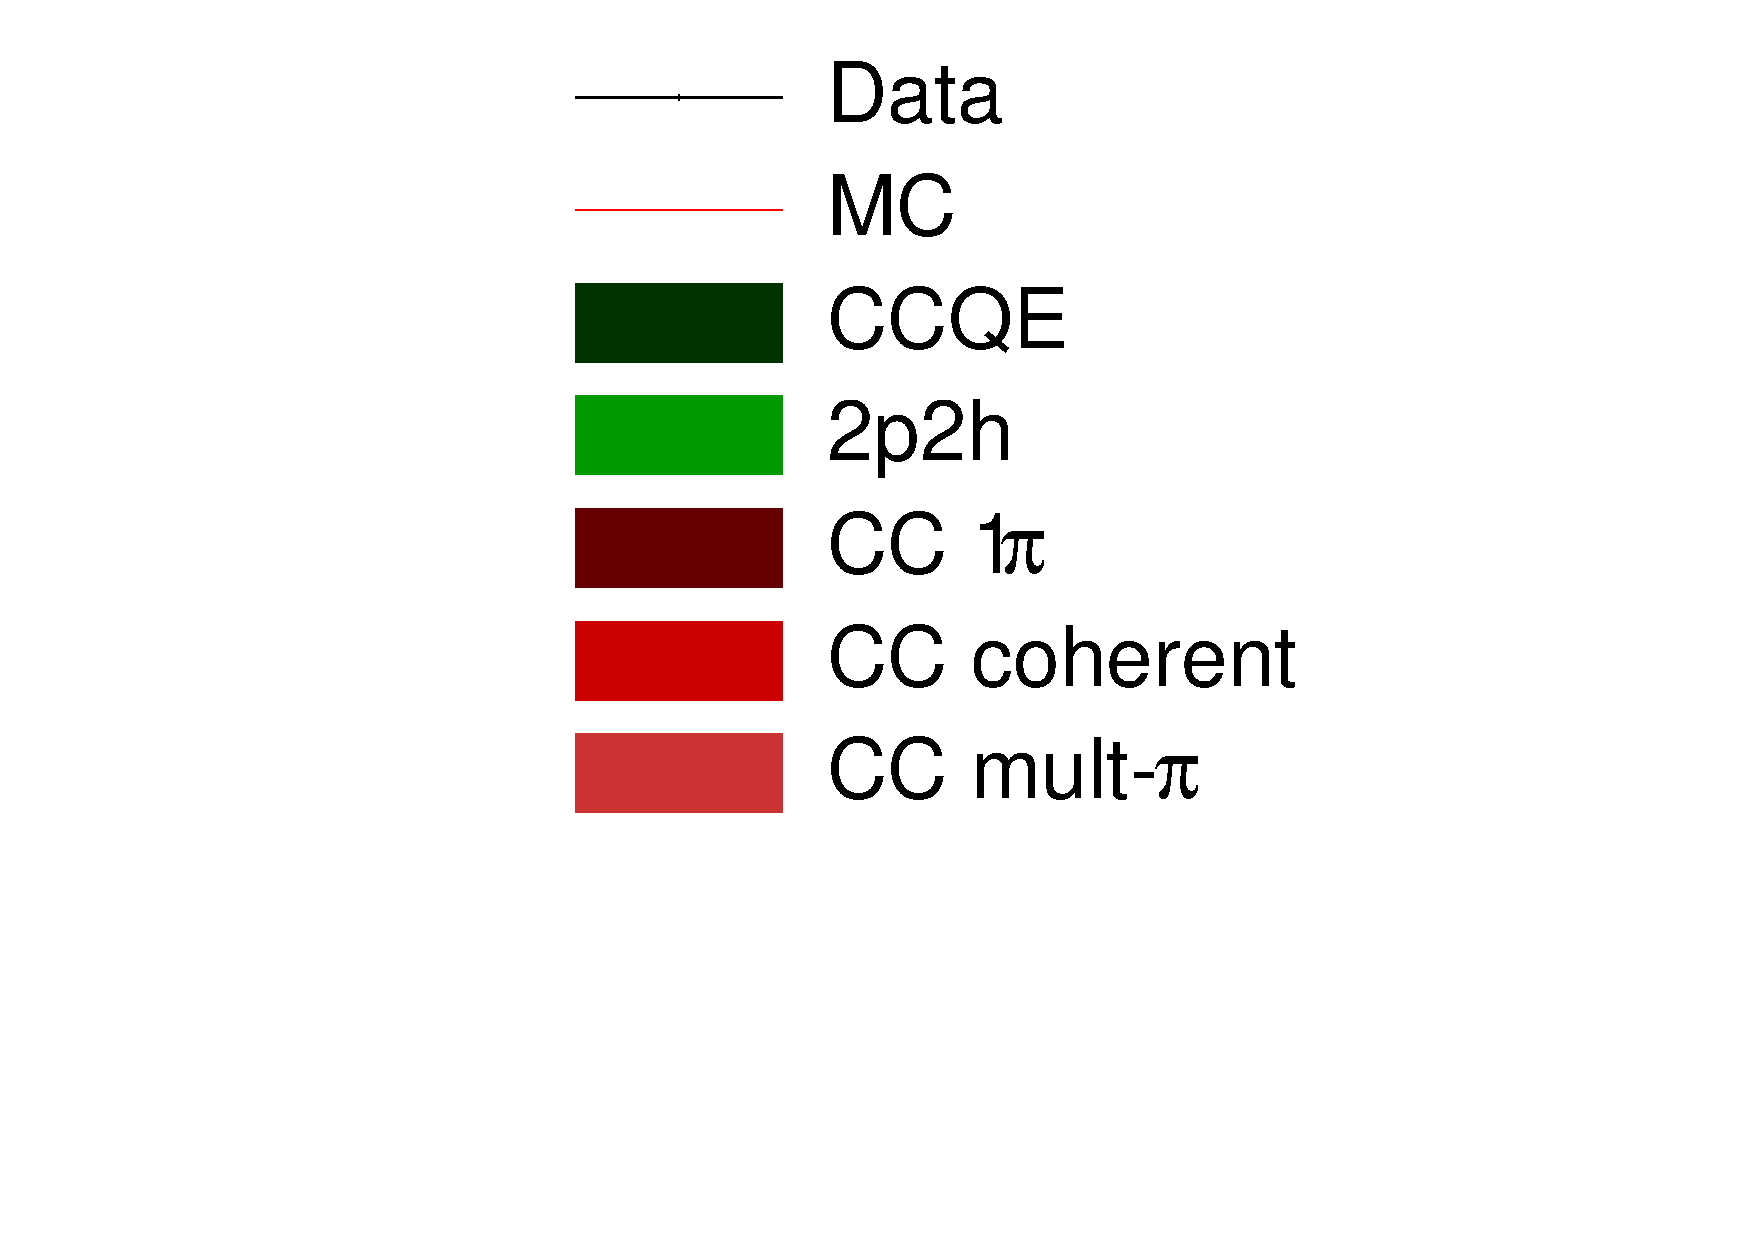
\includegraphics[width=\linewidth, trim={5mm 60mm 30mm 0mm}, clip]{figs/legend}
\end{subfigure}
\begin{subfigure}{.24\textwidth}
  \centering
  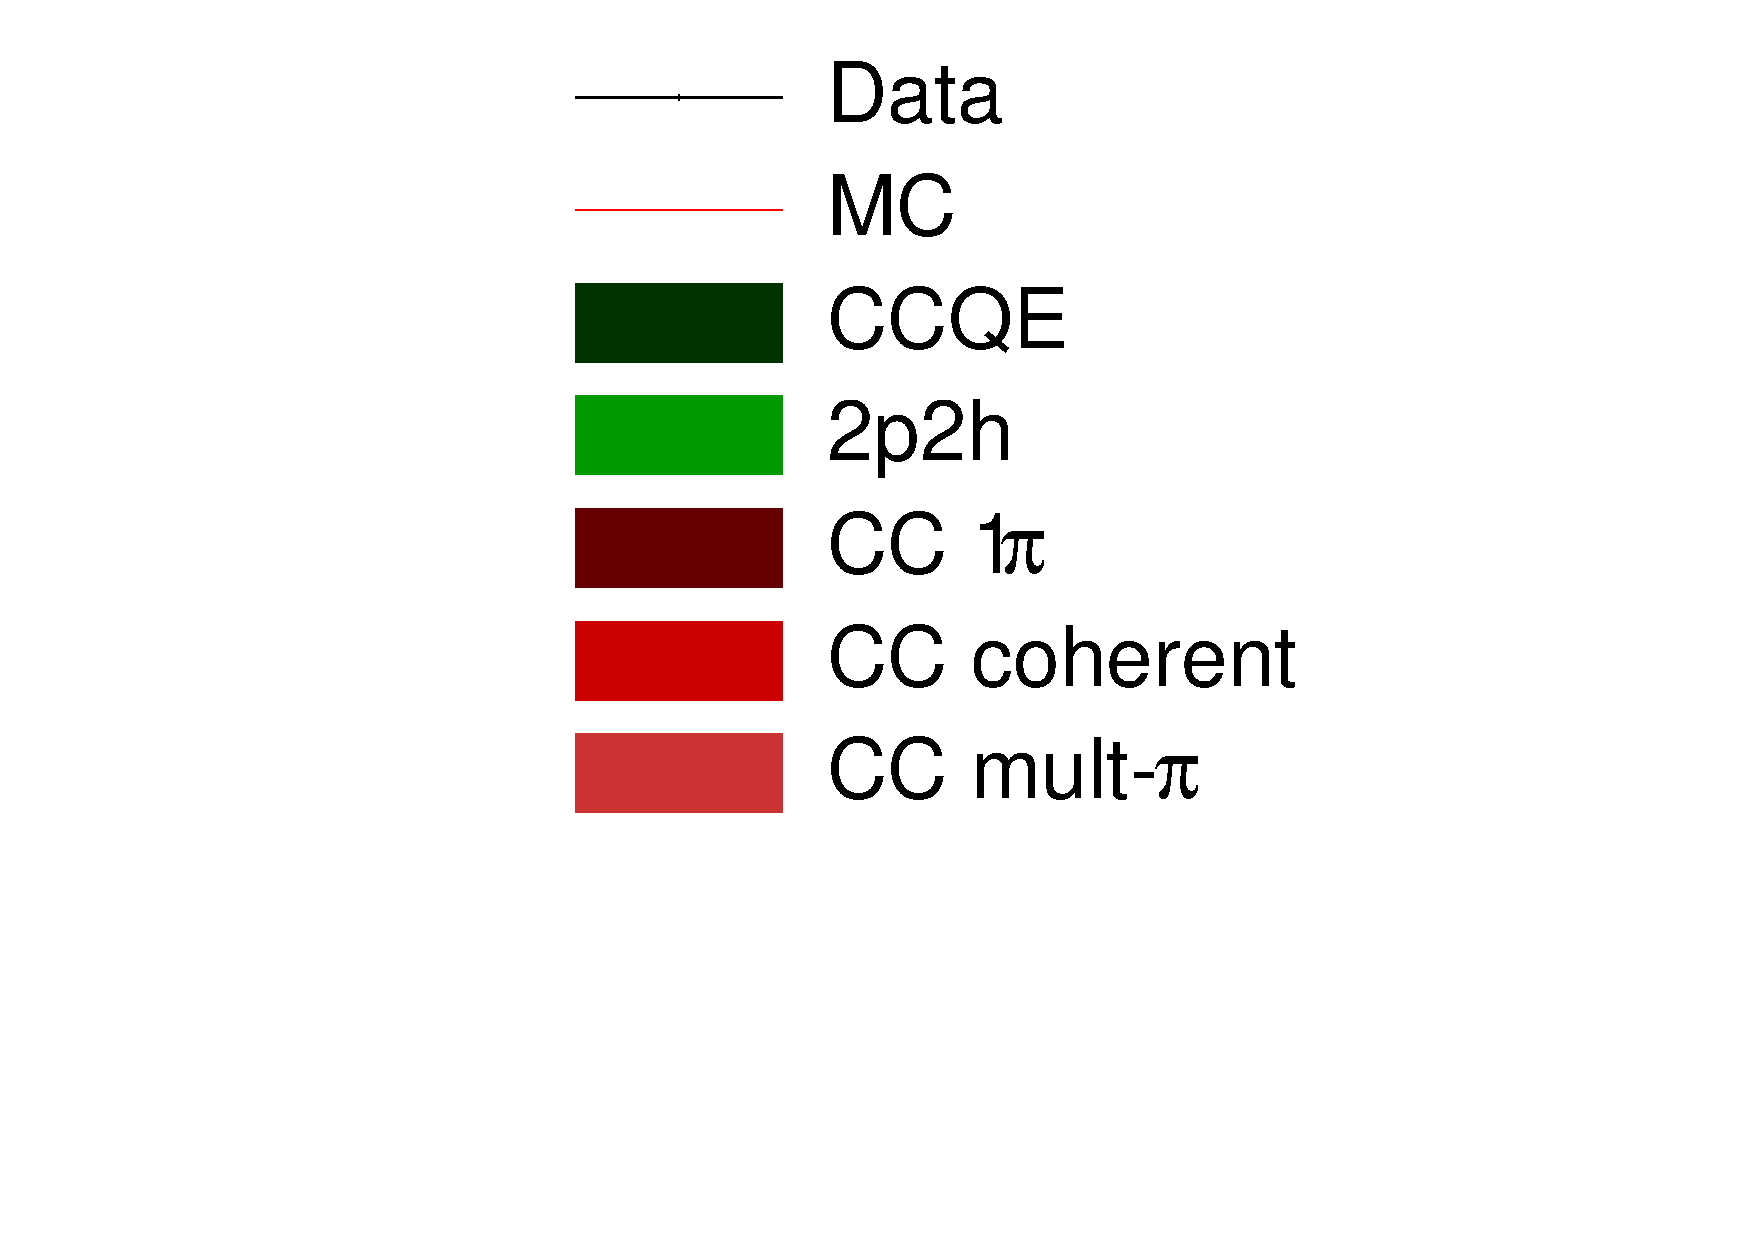
\includegraphics[width=\linewidth, trim={5mm 0mm 30mm 80mm}, clip]{figs/legend}
\end{subfigure}
\begin{subfigure}{.24\textwidth}
  \centering
  \includegraphics[width=\linewidth, trim={5mm 60mm 30mm 0mm}, clip]{figs/legend2}
\end{subfigure}
\begin{subfigure}{.24\textwidth}
  \centering
  \includegraphics[width=\linewidth, trim={5mm 0mm 30mm 80mm}, clip]{figs/legend2}
\end{subfigure}

\begin{subfigure}{0.49\textwidth}
  \centering
  \includegraphics[width=\textwidth]{figs/FGD1_numuCC_0pi_t}
  \caption{FGD1 FHC $\nu_{\mu}$ 0$\pi$}
\end{subfigure}
\begin{subfigure}{0.49\textwidth}
  \centering
  \includegraphics[width=\textwidth]{figs/FGD2_numuCC_0pi_t}
  \caption{FGD2 FHC $\nu_{\mu}$ 0$\pi$}
\end{subfigure}

\begin{subfigure}{0.49\textwidth}
  \centering
  \includegraphics[width=\textwidth]{figs/FGD1_numuCC_1pi_t}
  \caption{FGD1 FHC $\nu_{\mu}$ 1$\pi$}
\end{subfigure}
\centering
\begin{subfigure}{0.49\textwidth}
  \centering
  \includegraphics[width=\textwidth]{figs/FGD2_numuCC_1pi_t}
  \caption{FGD2 FHC $\nu_{\mu}$ 1$\pi$}
\end{subfigure}

\begin{subfigure}{0.49\textwidth}
  \centering
  \includegraphics[width=\textwidth]{figs/FGD1_numuCC_other_t}
  \caption{FGD1 FHC $\nu_{\mu}$ Other}
\end{subfigure}
\begin{subfigure}{0.49\textwidth}
  \centering
  \includegraphics[width=\textwidth]{figs/FGD2_numuCC_other_t}
  \caption{FGD2 $\nu_{\mu}$ Other}
\end{subfigure}
\caption{$\cos\theta_{\mu}$ projections of data and nominal MC broken down by interaction mode for FHC selections.}
\label{fig:tstack_fhcapp}
\end{figure}

\begin{figure}[!htbp]
\centering
\begin{subfigure}{.24\textwidth}
  \centering
  \includegraphics[width=\linewidth, trim={5mm 60mm 30mm 0mm}, clip]{figs/legend}
\end{subfigure}
\begin{subfigure}{.24\textwidth}
  \centering
  \includegraphics[width=\linewidth, trim={5mm 0mm 30mm 80mm}, clip]{figs/legend}
\end{subfigure}
\begin{subfigure}{.24\textwidth}
  \centering
  \includegraphics[width=\linewidth, trim={5mm 60mm 30mm 0mm}, clip]{figs/legend2}
\end{subfigure}
\begin{subfigure}{.24\textwidth}
  \centering
  \includegraphics[width=\linewidth, trim={5mm 0mm 30mm 80mm}, clip]{figs/legend2}
\end{subfigure}

\begin{subfigure}{0.49\textwidth}
  \centering
  \includegraphics[width=\textwidth]{figs/FGD1_anti-numuCC_0pi_t}
  \caption{FGD1 RHC $\bar{\nu_{\mu}}$ 0$\pi$}
\end{subfigure}
\begin{subfigure}{0.49\textwidth}
  \centering
  \includegraphics[width=\textwidth]{figs/FGD2_anti-numuCC_0pi_t}
  \caption{FGD2 RHC $\bar{\nu_{\mu}}$ 0$\pi$}
\end{subfigure}

\begin{subfigure}{0.49\textwidth}
  \centering
  \includegraphics[width=\textwidth]{figs/FGD1_anti-numuCC_1pi_t}
  \caption{FGD1 RHC $\bar{\nu_{\mu}}$ 1$\pi$}
\end{subfigure}
\centering
\begin{subfigure}{0.49\textwidth}
  \centering
  \includegraphics[width=\textwidth]{figs/FGD2_anti-numuCC_1pi_t}
  \caption{FGD2 RHC $\bar{\nu_{\mu}}$ 1$\pi$}
\end{subfigure}

\begin{subfigure}{0.49\textwidth}
  \centering
  \includegraphics[width=\textwidth]{figs/FGD1_anti-numuCC_other_t}
  \caption{FGD1 RHC $\bar{\nu_{\mu}}$ Other}
\end{subfigure}
\begin{subfigure}{0.49\textwidth}
  \centering
  \includegraphics[width=\textwidth]{figs/FGD2_anti-numuCC_other_t}
  \caption{FGD2 RHC $\bar{\nu_{\mu}}$ Other}
\end{subfigure}
\caption{$\cos\theta_{\mu}$ projections of data and nominal MC broken down by interaction mode for RHC \numub selections.}
\label{fig:tstack_rhc_numubapp}
\end{figure}

\begin{figure}[!htbp]
\centering
\begin{subfigure}{.24\textwidth}
  \centering
  \includegraphics[width=\linewidth, trim={5mm 60mm 30mm 0mm}, clip]{figs/legend}
\end{subfigure}
\begin{subfigure}{.24\textwidth}
  \centering
  \includegraphics[width=\linewidth, trim={5mm 0mm 30mm 80mm}, clip]{figs/legend}
\end{subfigure}
\begin{subfigure}{.24\textwidth}
  \centering
  \includegraphics[width=\linewidth, trim={5mm 60mm 30mm 0mm}, clip]{figs/legend2}
\end{subfigure}
\begin{subfigure}{.24\textwidth}
  \centering
  \includegraphics[width=\linewidth, trim={5mm 0mm 30mm 80mm}, clip]{figs/legend2}
\end{subfigure}

\begin{subfigure}{0.49\textwidth}
  \centering
  \includegraphics[width=\textwidth]{figs/FGD1_NuMuBkg_CC0pi_in_AntiNu_Mode_t}
  \caption{FGD1 RHC $\nu_{\mu}$ 0$\pi$}
\end{subfigure}
\begin{subfigure}{0.49\textwidth}
  \centering
  \includegraphics[width=\textwidth]{figs/FGD2_NuMuBkg_CC0pi_in_AntiNu_Mode_t}
  \caption{FGD2 RHC $\nu_{\mu}$ 0$\pi$}
\end{subfigure}

\begin{subfigure}{0.49\textwidth}
  \centering
  \includegraphics[width=\textwidth]{figs/FGD1_NuMuBkg_CC1pi_in_AntiNu_Mode_t}
  \caption{FGD1 RHC $\nu_{\mu}$ 1$\pi$}
\end{subfigure}
\begin{subfigure}{0.49\textwidth}
  \centering
  \includegraphics[width=\textwidth]{figs/FGD2_NuMuBkg_CC1pi_in_AntiNu_Mode_t}
  \caption{FGD2 RHC $\nu_{\mu}$ 1$\pi$}
\end{subfigure}

\begin{subfigure}{0.49\textwidth}
  \centering
  \includegraphics[width=\textwidth]{figs/FGD1_NuMuBkg_CCOther_in_AntiNu_Mode_t}
  \caption{FGD1 RHC $\nu_{\mu}$ Other}
\end{subfigure}
\begin{subfigure}{0.49\textwidth}
  \centering
  \includegraphics[width=\textwidth]{figs/FGD2_NuMuBkg_CCOther_in_AntiNu_Mode_t}
  \caption{FGD2 RHC $\nu_{\mu}$ Other}
\end{subfigure}
\caption{$\cos\theta_{\mu}$ projections of data and nominal MC broken down by interaction mode for RHC \numu selections.}
\label{fig:tstack_rhc_numuapp}
\end{figure}